\documentclass[acmsmall, screen]{acmart}

\usepackage{booktabs}
\usepackage{cleveref}
\usepackage{enumitem}
\usepackage{subcaption}
\usepackage{xspace}

\usepackage{bbm}
\usepackage{stmaryrd}
\usepackage{mathtools}
\usepackage{mathpartir}

\bibliographystyle{ACM-Reference-Format}
\citestyle{acmauthoryear}
\setcopyright{none}

%
% utilities
%
\definecolor{hole}{RGB}{162,85,162}
\definecolor{cursorhighlight}{RGB}{230,255,230}
\definecolor{cursor}{RGB}{76,170,76}
\newcommand{\mathcolorbox}[2]{{\fboxsep=1pt\colorbox{#1}{$\displaystyle #2$}}}

%
% judgments
%

% judgments
\newcommand{\judgment}[3]{\inferrule[#3]{#1}{#2}}
\newcommand{\judgbox}[1]{\noindent \fbox{$#1$}}

% equality
\newcommand{\equal}[2]{\ensuremath{#1 = #2}}
\newcommand{\notEqual}[2]{\ensuremath{#1 \neq #2}}

% consistency
\newcommand{\consistent}[2]{\ensuremath{#1 \sim #2}}
\newcommand{\inconsistentRel}{\ensuremath{\nsim}}
\newcommand{\inconsistent}[2]{\ensuremath{#1 \inconsistentRel #2}}

% matching
\newcommand{\matchedRel}[1]{\ensuremath{\blacktriangleright_{#1}}}
\newcommand{\notMatchedRel}[1]{\ensuremath{\blacktriangleright_{\centernot#1}}}
\newcommand{\matchedArrowRel}{\ensuremath{\matchedRel{\to}}}
\newcommand{\notMatchedArrowRel}{\ensuremath{\notMatchedRel{\to}}}
\newcommand{\matchedArrow}[3]{\ensuremath{#1 \matchedArrowRel \TArrow{#2}{#3}}}
\newcommand{\notMatchedArrow}[1]{\ensuremath{#1 \notMatchedArrowRel}}
\newcommand{\matchedPairRel}{\ensuremath{\matchedRel{\times}}}
\newcommand{\notMatchedPairRel}{\ensuremath{\notMatchedRel{\times}}}
\newcommand{\matchedPair}[3]{\ensuremath{#1 \matchedPairRel \TPair{#2}{#3}}}
\newcommand{\notMatchedPair}[3]{\ensuremath{#1 \notMatchedPairRel \TPair{#2}{#3}}}

% contexts
\newcommand{\ctx}{\ensuremath{\Gamma}}
\newcommand{\extendCtx}[3]{\ensuremath{#1 , ~\assignType{#2}{#3}}}
\DeclareMathOperator{\dom}{dom}
\newcommand{\inCtx}[3]{\ensuremath{\assignType{#2}{#3} \in #1}}
\newcommand{\notInCtx}[2]{\ensuremath{#2 \not\in \dom(#1)}}
\newcommand{\withCtx}[2]{\ensuremath{#1 \vdash #2}}

% typing
\newcommand{\assignType}[2]{\ensuremath{#1 : #2}}
\newcommand{\ctxAssignType}[3]{\ensuremath{\withCtx{#1}{\assignType{#2}{#3}}}}
\newcommand{\synType}[2]{\ensuremath{#1 \Rightarrow #2}}
\newcommand{\notSynType}[2]{\ensuremath{#1 \not\Rightarrow #2}}
\newcommand{\ctxSynType}[3]{\ensuremath{\withCtx{#1}{\synType{#2}{#3}}}}
\newcommand{\ctxNotSynType}[3]{\ensuremath{\withCtx{#1}{\notSynType{#2}{#3}}}}
\newcommand{\anaType}[2]{\ensuremath{#1 \Leftarrow #2}}
\newcommand{\notAnaType}[2]{\ensuremath{#1 \not\Leftarrow #2}}
\newcommand{\ctxAnaType}[3]{\ensuremath{\withCtx{#1}{\anaType{#2}{#3}}}}
\newcommand{\ctxNotAnaType}[3]{\ensuremath{\withCtx{#1}{\notAnaType{#2}{#3}}}}

% typing patterns
\newcommand{\ctxSynPat}[3]{\ensuremath{\withCtx{#1}{\synType{#2}{#3}}}}
\newcommand{\ctxAnaPat}[4]{\ensuremath{\withCtx{#1}{\anaType{#2}{#3 ; #4}}}}
\newcommand{\PMV}{\ensuremath{p}}
\newcommand{\PMName}{{\normalfont\textsf{UPat}}}
\newcommand{\TUnknownSwitch}{\ensuremath{\?^{\Rightarrow}}}

% subsumable
\newcommand{\subsumable}[1]{\ensuremath{#1 ~{\normalfont{\normalfont\textsf{subsumable}}}}}

% mark erasure
\newcommand{\erase}[1]{\ensuremath{#1^{\square}}}
\newcommand{\erasesTo}[2]{\ensuremath{#1^{\square} = #2}}

% marking
\newcommand{\synFixedInto}[3]{\ensuremath{\synType{#1 \looparrowright #2}{#3}}}
\newcommand{\ctxSynFixedInto}[4]{\ensuremath{\withCtx{#1}{\synFixedInto{#2}{#3}{#4}}}}
\newcommand{\anaFixedInto}[3]{\ensuremath{\anaType{#1 \looparrowright #2}{#3}}}
\newcommand{\ctxAnaFixedInto}[4]{\ensuremath{\withCtx{#1}{\anaFixedInto{#2}{#3}{#4}}}}

% marking image
\newcommand{\image}[1]{\ensuremath{#1^{\circ}}}
\newcommand{\imageIs}[2]{\ensuremath{\image{#1} = #2}}
\newcommand{\imageIsNot}[2]{\ensuremath{\image{#1} \neq #2}}

% cursor erasure
\newcommand{\cursorErase}[1]{\ensuremath{#1^{\diamond}}}
\newcommand{\cursorErasesTo}[2]{\ensuremath{#1^{\diamond} = #2}}

% zippered expression well-formedness
\newcommand{\zWellFormed}[1]{\ensuremath{#1 ~{\normalfont\textsf{WF}}}}

% 
% types
%
\newcommand{\TMName}{{\normalfont\textsf{Type}}}
\newcommand{\TMSet}{\ensuremath{T}}
\newcommand{\TMV}{\ensuremath{\tau}}

\newcommand{\joinRel}{\sqcup}
\newcommand{\noJoinRel}{\centernot\sqcup}
\newcommand{\TJoin}[2]{\ensuremath{#1 \joinRel #2}}

\DeclareMathOperator{\?}{?}
\newcommand{\TUnknown}{\ensuremath{\?}}
\newcommand{\TNum}{\ensuremath{{\normalfont\textsf{num}}}}
\newcommand{\TVar}{\ensuremath{{\normalfont\textsf{var}}}}
\newcommand{\TBool}{\ensuremath{{\normalfont\textsf{bool}}}}
\newcommand{\TArrow}[2]{\ensuremath{#1 \to #2}}
\newcommand{\TPair}[2]{\ensuremath{#1 \times #2}}

%
% external expressions
%
\newcommand{\EMName}{{\normalfont\textsf{UExp}}}
\newcommand{\EMSet}{\ensuremath{E}}
\newcommand{\EMV}{\ensuremath{e}}

% holes
\newcommand{\EEHole}{\ensuremath{\ECEHole}}

% integers
\newcommand{\ENum}[1]{\ensuremath{\ECNum{#1}}}
\newcommand{\ENumMV}{\ensuremath{\ECNumMV}}
\newcommand{\EOpPlus}{\ensuremath{\ECOpPlus}}
\newcommand{\EPlus}[2]{\ensuremath{\ECPlus{#1}{#2}}}

% booleans
\newcommand{\ETrue}{\ensuremath{\ECTrue}}
\newcommand{\EFalse}{\ensuremath{\ECFalse}}
\newcommand{\EIf}[3]{\ensuremath{\ECIf{#1}{#2}{#3}}}

% lambdas
\newcommand{\ELam}[3]{\ensuremath{\ECLam{#1}{#2}{#3}}}
\newcommand{\EAp}[2]{\ensuremath{\ECAp{#1}{#2}}}

% pairs
\newcommand{\EPair}[2]{\ensuremath{\ECPair{#1}{#2}}}
\newcommand{\EProjL}[1]{\ensuremath{\ECProjL{#1}}}
\newcommand{\EProjR}[1]{\ensuremath{\ECProjR{#1}}}

% let
\newcommand{\ELet}[3]{\ensuremath{\ECLet{#1}{#2}{#3}}}

%
% cursor types
%
\newcommand{\ZTMName}{{\normalfont\textsf{ZType}}}
\newcommand{\ZTMSet}{\ensuremath{\hat{T}}}
\newcommand{\ZTMV}{\ensuremath{\hat{\tau}}}

% cursor
\newcommand{\ZTCursor}[1]{\ensuremath{\ZCursor{#1}}}

% arrow
\newcommand{\ZTArrowL}[2]{\ensuremath{\TArrow{#1}{#2}}}
\newcommand{\ZTArrowR}[2]{\ensuremath{\TArrow{#1}{#2}}}

%
% marked expressions
%
\newcommand{\ECMName}{{\normalfont\textsf{MExp}}}
\newcommand{\ECMSet}{\ensuremath{\check{E}}}
\newcommand{\ECMV}{\ensuremath{\check{e}}}

% holes
\newcommand{\ECEHole}{\ensuremath{\textcolor{hole}{\bm{\llparenthesis}}\textcolor{hole}{\bm{\rrparenthesis}}}}

% integers
\newcommand{\ECNum}[1]{\ensuremath{\underline{#1}}}
\newcommand{\ECNumMV}{\ensuremath{\ECNum{n}}}
\newcommand{\ECOpPlus}{\ensuremath{+}}
\newcommand{\ECPlus}[2]{\ensuremath{#1 \ECOpPlus #2}}

% booleans
\newcommand{\ECTrue}{\ensuremath{{\normalfont\textsf{tt}}}}
\newcommand{\ECFalse}{\ensuremath{{\normalfont\textsf{ff}}}}
\newcommand{\ECIf}[3]{\ensuremath{#1 ~?~ #2 : #3}}

% lambdas
\newcommand{\ECLam}[3]{\ensuremath{\lambda #1 : #2. ~#3}}
\newcommand{\ECAp}[2]{\ensuremath{#1 ~#2}}
\newcommand{\ECApNonMatched}[2]{\ensuremath{\ECAp{\ECInconType{#1}}{#2}}}
\newcommand{\ECApNonMatchedAlt}[2]{\ensuremath{\textcolor{red}{[}\ECAp{#1}{#2}\textcolor{red}{]}}}
\newcommand{\ECApNonMatchedAltAlt}[2]{\ensuremath{\ECAp{\ECInconMatchedArrow{#1}}{#2}}}

% pairs
\newcommand{\ECPair}[2]{\ensuremath{(#1, #2)}}
\newcommand{\ECProjL}[1]{\ensuremath{\pi_1 #1}}
\newcommand{\ECProjR}[1]{\ensuremath{\pi_2 #1}}

% let
\newcommand{\ECLet}[3]{\ensuremath{\textsf{let}~ #1 = #2 ~\textsf{in}~ #3}}

% errors
\newcommand{\MRUnbound}{\ensuremath{\mathsmaller{\mathsmaller{\mathsmaller{\square}}}}}
\newcommand{\MRInconType}{\ensuremath{\mathsmaller{\inconsistentRel}}}
\newcommand{\MRInconBr}{\ensuremath{\mathlarger{\noJoinRel}}}

\newcommand{\ECMarked}[2]{\ensuremath{\textcolor{red}{\bm{\llparenthesis}}#1\textcolor{red}{\bm{\rrparenthesis}_{#2}}}}
\newcommand{\ECMarkedUnbound}[1]{\ensuremath{\ECMarked{#1}{\MRUnbound}}}
\newcommand{\ECMarkedInconType}[1]{\ensuremath{\ECMarked{#1}{\MRInconType}}}
\newcommand{\ECMarkedInconBr}[1]{\ensuremath{\ECMarked{#1}{\MRInconBr}}}

\newcommand{\ECUnbound}[1]{\ensuremath{\ECMarkedUnbound{#1}}}
\newcommand{\ECInconType}[1]{\ensuremath{\ECMarkedInconType{#1}}}
\newcommand{\ECInconBr}[3]{\ensuremath{\ECMarkedInconBr{\ECIf{#1}{#2}{#3}}}}

\newcommand{\ECInconMatched}[2]{\ensuremath{\ECMarked{#1}{#2}}}
\newcommand{\ECInconMatchedArrow}[1]{\ensuremath{\ECInconMatched{#1}{\notMatchedArrowRel}}}
\newcommand{\ECInconMatchedPair}[1]{\ensuremath{\ECInconMatched{#1}{\notMatchedPairRel}}}

%
% zippered expressions
%
\newcommand{\ZMName}{{\normalfont\textsf{ZExp}}}
\newcommand{\ZMSet}{\ensuremath{\hat{E}}}
\newcommand{\ZMV}{\ensuremath{\hat{e}}}

% cursor
\newcommand{\ZCursor}[1]{\ensuremath{\mathcolorbox{cursorhighlight}{\textcolor{cursor}{\bm{\triangleright}}#1\textcolor{cursor}{\bm{\triangleleft}}}}}

% integers
\newcommand{\ZPlusL}[2]{\ensuremath{\ECPlus{#1}{#2}}}
\newcommand{\ZPlusR}[2]{\ensuremath{\ECPlus{#1}{#2}}}

% lambdas
\newcommand{\ZLamT}[3]{\ensuremath{\ECLam{#1}{#2}{#3}}}
\newcommand{\ZLamE}[3]{\ensuremath{\ECLam{#1}{#2}{#3}}}
\newcommand{\ZApL}[2]{\ensuremath{\ECAp{#1}{#2}}}
\newcommand{\ZApR}[2]{\ensuremath{\ECAp{#1}{#2}}}
\newcommand{\ZApNonMatchedL}[2]{\ensuremath{\ECApNonMatched{#1}{#2}}}
\newcommand{\ZApNonMatchedR}[2]{\ensuremath{\ECApNonMatched{#1}{#2}}}

% booleans
\newcommand{\ZIfC}[3]{\ensuremath{\ECIf{#1}{#2}{#3}}}
\newcommand{\ZIfL}[3]{\ensuremath{\ECIf{#1}{#2}{#3}}}
\newcommand{\ZIfR}[3]{\ensuremath{\ECIf{#1}{#2}{#3}}}
\newcommand{\ZInconBrC}[3]{\ensuremath{\ECInconBr{#1}{#2}{#3}}}
\newcommand{\ZInconBrL}[3]{\ensuremath{\ECInconBr{#1}{#2}{#3}}}
\newcommand{\ZInconBrR}[3]{\ensuremath{\ECInconBr{#1}{#2}{#3}}}

% let
\newcommand{\ZLetL}[3]{\ensuremath{\ECLet{#1}{#2}{#3}}}
\newcommand{\ZLetR}[3]{\ensuremath{\ECLet{#1}{#2}{#3}}}

% errors
\newcommand{\ZUnbound}[1]{\ensuremath{\ECUnbound{#1}}}
\newcommand{\ZInconType}[1]{\ensuremath{\ECInconType{#1}}}
\newcommand{\ZInconBr}[3]{\ensuremath{\ECInconBr{#1}{#2}{#3}}}

%
% actions
%
\newcommand{\movements}[1]{\ensuremath{#1 ~{\normalfont\textsf{movements}}}}
\newcommand{\tshape}[1]{\ensuremath{#1 ~{\normalfont\textsf{tshape}}}}
\newcommand{\eshape}[1]{\ensuremath{#1 ~{\normalfont\textsf{eshape}}}}

% actions
\newcommand{\AMName}{{\normalfont\textsf{Action}}}
\newcommand{\AMV}{\ensuremath{\alpha}}
\newcommand{\AMove}[1]{\ensuremath{{\normalfont\textsf{move $#1$}}}}
\newcommand{\ADel}{\ensuremath{{\normalfont\textsf{del}}}}
\newcommand{\ACon}[1]{\ensuremath{{\normalfont\textsf{construct $#1$}}}}

% iterated actions
\newcommand{\AIMName}{{\normalfont\textsf{ActionList}}}
\newcommand{\AIMV}{\ensuremath{\overline{\alpha}}}
\newcommand{\AINil}{\ensuremath{\cdot}}
\newcommand{\AICons}[2]{\ensuremath{#1; #2}}

% directions
\newcommand{\MMName}{{\normalfont\textsf{Dir}}}
\newcommand{\MMV}{\ensuremath{\delta}}
\newcommand{\MChild}[1]{\ensuremath{{\normalfont\textsf{child $#1$}}}}
\newcommand{\MChildNMV}{\ensuremath{n}}
\newcommand{\MParent}{\ensuremath{{\normalfont\textsf{parent}}}}

% shapes
\newcommand{\SMName}{{\normalfont\textsf{Shape}}}
\newcommand{\SMV}{\ensuremath{\psi}}

\newcommand{\STArrowL}{\ensuremath{{\normalfont\textsf{arrow\textsubscript{L}}}}}
\newcommand{\STArrowR}{\ensuremath{{\normalfont\textsf{arrow\textsubscript{R}}}}}
\newcommand{\STNum}{\ensuremath{{\normalfont\textsf{num}}}}
\newcommand{\STBool}{\ensuremath{{\normalfont\textsf{bool}}}}

\newcommand{\SVar}[1]{\ensuremath{{\normalfont\textsf{var $#1$}}}}
\newcommand{\SLam}[1]{\ensuremath{{\normalfont\textsf{lam $#1$}}}}
\newcommand{\SApL}{\ensuremath{{\normalfont\textsf{ap\textsubscript{L}}}}}
\newcommand{\SApR}{\ensuremath{{\normalfont\textsf{ap\textsubscript{R}}}}}
\newcommand{\SLetL}[1]{\ensuremath{{\normalfont\textsf{let\textsubscript{L} $#1$}}}}
\newcommand{\SLetR}[1]{\ensuremath{{\normalfont\textsf{let\textsubscript{R} $#1$}}}}
\newcommand{\SLit}[1]{\ensuremath{{\normalfont\textsf{lit $#1$}}}}
\newcommand{\SPlusL}{\ensuremath{{\normalfont\textsf{plus\textsubscript{L}}}}}
\newcommand{\SPlusR}{\ensuremath{{\normalfont\textsf{plus\textsubscript{R}}}}}
\newcommand{\STrue}{\ensuremath{{\normalfont\textsf{true}}}}
\newcommand{\SFalse}{\ensuremath{{\normalfont\textsf{false}}}}
\newcommand{\SIfC}{\ensuremath{{\normalfont\textsf{if\textsubscript{C}}}}}
\newcommand{\SIfL}{\ensuremath{{\normalfont\textsf{if\textsubscript{L}}}}}
\newcommand{\SIfR}{\ensuremath{{\normalfont\textsf{if\textsubscript{R}}}}}


%
% untyped action judgments
%
\newcommand{\AUAction}[3]{\ensuremath{#1 \xrightarrow{#3} #2}}
\newcommand{\AUActionIter}[3]{\ensuremath{#1 \xrightarrow{#3}* #2}}

% movement
\newcommand{\AUMChild}[3]{\ensuremath{\AUAction{#1}{#2}{\AMove{\MChild{#3}}}}}
\newcommand{\AUMParent}[2]{\ensuremath{\AUAction{#1}{#2}{\AMove{\MParent}}}}

% deletion
\newcommand{\AUDel}[2]{\ensuremath{\AUAction{#1}{#2}{\ADel}}}

% construction
\newcommand{\AUCon}[3]{\ensuremath{\AUAction{#1}{#2}{\ACon{#3}}}}

%
% type actions
%
\newcommand{\AUTAction}[3]{\ensuremath{\AUAction{#1}{#2}{#3}}}
\newcommand{\AUTActionIter}[3]{\ensuremath{\AUActionIter{#1}{#2}{#3}}}

% movement
\newcommand{\AUTMChild}[3]{\ensuremath{\AUMChild{\ZTCursor{#1}}{#2}{#3}}}
\newcommand{\AUTMParent}[2]{\ensuremath{\AUMParent{#1}{\ZTCursor{#2}}}}
\newcommand{\AUTMArrowChildL}[2]{\ensuremath{\AUTMChild{\TArrow{#1}{#2}}{\ZTArrowL{\ZTCursor{#1}}{#2}}{1}}}
\newcommand{\AUTMArrowChildR}[2]{\ensuremath{\AUTMChild{\TArrow{#1}{#2}}{\ZTArrowR{#2}{\ZTCursor{#1}}}{2}}}
\newcommand{\AUTMArrowParentL}[2]{\ensuremath{\AUTMParent{\ZTArrowL{\ZTCursor{#1}}{#2}}{\TArrow{#1}{#2}}}}
\newcommand{\AUTMArrowParentR}[2]{\ensuremath{\AUTMParent{\ZTArrowR{#2}{\ZTCursor{#1}}}{\TArrow{#1}{#2}}}}

% deletion
\newcommand{\AUTDel}[1]{\ensuremath{\AUDel{\ZTCursor{#1}}{\ZTCursor{\TUnknown}}}}

% construction
\newcommand{\AUTConArrowL}[1]{\ensuremath{\AUCon{\ZTCursor{#1}}{\ZTArrowR{#1}{\ZTCursor{\TUnknown}}}{\STArrowL}}}
\newcommand{\AUTConArrowR}[1]{\ensuremath{\AUCon{\ZTCursor{#1}}{\ZTArrowR{\ZTCursor{\TUnknown}}{#1}}{\STArrowR}}}
\newcommand{\AUTConNum}{\ensuremath{\AUCon{\ZTCursor{\TUnknown}}{\ZTCursor{\TNum}}{\STNum}}}
\newcommand{\AUTConBool}{\ensuremath{\AUCon{\ZTCursor{\TUnknown}}{\ZTCursor{\TBool}}{\STBool}}}

%
% untyped expression actions
%
\newcommand{\AUEAction}[3]{\ensuremath{\AUAction{#1}{#2}{#3}}}
\newcommand{\AUEActionIter}[3]{\ensuremath{\AUActionIter{#1}{#2}{#3}}}

% movement
\newcommand{\AUEMove}[3]{\ensuremath{\AUEAction{#1}{#2}{\AMove{\MMV}}}}
\newcommand{\AUEMChild}[3]{\ensuremath{\AUMChild{\ZCursor{#1}}{#2}{#3}}}
\newcommand{\AUEMParent}[2]{\ensuremath{\AUMParent{#1}{\ZCursor{#2}}}}

\newcommand{\AUEMLamChildT}[3]{\ensuremath{\AUEMChild{\ELam{#1}{#2}{#3}}{\ZLamT{#1}{\ZTCursor{#2}}{#3}}{1}}}
\newcommand{\AUEMLamChildE}[3]{\ensuremath{\AUEMChild{\ELam{#1}{#2}{#3}}{\ZLamE{#1}{#2}{\ZCursor{#3}}}{2}}}
\newcommand{\AUEMLamParentT}[3]{\ensuremath{\AUEMParent{\ZLamT{#1}{\ZTCursor{#2}}{#3}}{\ELam{#1}{#2}{#3}}}}
\newcommand{\AUEMLamParentE}[3]{\ensuremath{\AUEMParent{\ZLamE{#1}{#2}{\ZCursor{#3}}}{\ELam{#1}{#2}{#3}}}}
\newcommand{\AUEMApChildL}[2]{\ensuremath{\AUEMChild{\EAp{#1}{#2}}{\ZApL{\ZCursor{#1}}{#2}}{1}}}
\newcommand{\AUEMApChildR}[2]{\ensuremath{\AUEMChild{\EAp{#1}{#2}}{\ZApR{#1}{\ZCursor{#2}}}{2}}}
\newcommand{\AUEMApParentL}[2]{\ensuremath{\AUEMParent{\ZApL{\ZCursor{#1}}{#2}}{\EAp{#1}{#2}}}}
\newcommand{\AUEMApParentR}[2]{\ensuremath{\AUEMParent{\ZApR{#1}{\ZCursor{#2}}}{\EAp{#1}{#2}}}}
\newcommand{\AUEMLetChildL}[3]{\ensuremath{\AUEMChild{\ELet{#1}{#2}{#3}}{\ZLetL{#1}{\ZCursor{#2}}{#3}}{1}}}
\newcommand{\AUEMLetChildR}[3]{\ensuremath{\AUEMChild{\ELet{#1}{#2}{#3}}{\ZLetR{#1}{#2}{\ZCursor{#3}}}{2}}}
\newcommand{\AUEMLetParentL}[3]{\ensuremath{\AUEMParent{\ZLetL{#1}{\ZCursor{#2}}{#3}}{\ELet{#1}{#2}{#3}}}}
\newcommand{\AUEMLetParentR}[3]{\ensuremath{\AUEMParent{\ZLetR{#1}{#2}{\ZCursor{#3}}}{\ELet{#1}{#2}{#3}}}}
\newcommand{\AUEMPlusChildL}[2]{\ensuremath{\AUEMChild{\EPlus{#1}{#2}}{\ZPlusL{\ZCursor{#1}}{#2}}{1}}}
\newcommand{\AUEMPlusChildR}[2]{\ensuremath{\AUEMChild{\EPlus{#1}{#2}}{\ZPlusR{#1}{\ZCursor{#2}}}{2}}}
\newcommand{\AUEMPlusParentL}[2]{\ensuremath{\AUEMParent{\ZPlusL{\ZCursor{#1}}{#2}}{\EPlus{#1}{#2}}}}
\newcommand{\AUEMPlusParentR}[2]{\ensuremath{\AUEMParent{\ZPlusR{#1}{\ZCursor{#2}}}{\EPlus{#1}{#2}}}}
\newcommand{\AUEMIfChildC}[3]{\ensuremath{\AUEMChild{\EIf{#1}{#2}{#3}}{\ZIfC{\ZCursor{#1}}{#2}{#3}}{1}}}
\newcommand{\AUEMIfChildL}[3]{\ensuremath{\AUEMChild{\EIf{#1}{#2}{#3}}{\ZIfL{#1}{\ZCursor{#2}}{#3}}{2}}}
\newcommand{\AUEMIfChildR}[3]{\ensuremath{\AUEMChild{\EIf{#1}{#2}{#3}}{\ZIfR{#1}{#2}{\ZCursor{#3}}}{3}}}
\newcommand{\AUEMIfParentC}[3]{\ensuremath{\AUEMParent{\ZIfC{\ZCursor{#1}}{#2}{#3}}{\EIf{#1}{#2}{#3}}}}
\newcommand{\AUEMIfParentL}[3]{\ensuremath{\AUEMParent{\ZIfL{#1}{\ZCursor{#2}}{#3}}{\EIf{#1}{#2}{#3}}}}
\newcommand{\AUEMIfParentR}[3]{\ensuremath{\AUEMParent{\ZIfR{#1}{#2}{\ZCursor{#3}}}{\EIf{#1}{#2}{#3}}}}

% deletion
\newcommand{\AUEDel}[1]{\ensuremath{\AUDel{\ZCursor{#1}}{\ZCursor{\EEHole}}}}

% construction
\newcommand{\AUEConVar}[1]{\ensuremath{\AUCon{\ZCursor{\EEHole}}{\ZCursor{#1}}{\SVar{#1}}}}
\newcommand{\AUEConLam}[2]{\ensuremath{\AUCon{\ZCursor{#2}}{\ZLamT{#1}{\ZTCursor{\TUnknown}}{#2}}{\SLam{#1}}}}
\newcommand{\AUEConApL}[1]{\ensuremath{\AUCon{\ZCursor{#1}}{\ZApR{#1}{\ZCursor{\EEHole}}}{\SApL}}}
\newcommand{\AUEConApR}[1]{\ensuremath{\AUCon{\ZCursor{#1}}{\ZApR{\ZCursor{\EEHole}}{#1}}{\SApR}}}
\newcommand{\AUEConLetL}[2]{\ensuremath{\AUCon{\ZCursor{#2}}{\ZLetL{#1}{#2}{\ZCursor{\EEHole}}}{\SLetL{#1}}}}
\newcommand{\AUEConLetR}[2]{\ensuremath{\AUCon{\ZCursor{#2}}{\ZLetR{#1}{\ZCursor{\EEHole}}{#2}}{\SLetR{#1}}}}
\newcommand{\AUEConNum}[1]{\ensuremath{\AUCon{\ZCursor{\EEHole}}{\ZCursor{#1}}{\SLit{#1}}}}
\newcommand{\AUEConPlusL}[1]{\ensuremath{\AUCon{\ZCursor{#1}}{\ZPlusR{#1}{\ZCursor{\EEHole}}}{\SPlusL}}}
\newcommand{\AUEConPlusR}[1]{\ensuremath{\AUCon{\ZCursor{#1}}{\ZPlusR{\ZCursor{\EEHole}}{#1}}{\SPlusR}}}
\newcommand{\AUEConTrue}{\ensuremath{\AUCon{\ZCursor{\EEHole}}{\ZCursor{\ETrue}}{\STrue}}}
\newcommand{\AUEConFalse}{\ensuremath{\AUCon{\ZCursor{\EEHole}}{\ZCursor{\EFalse}}{\SFalse}}}
\newcommand{\AUEConIfC}[1]{\ensuremath{\AUCon{\ZCursor{#1}}{\ZIfC{#1}{\ZCursor{\EEHole}}{\EEHole}}{\SIfC}}}
\newcommand{\AUEConIfL}[1]{\ensuremath{\AUCon{\ZCursor{#1}}{\ZIfC{\ZCursor{\EEHole}}{#1}{\EEHole}}{\SIfC}}}
\newcommand{\AUEConIfR}[1]{\ensuremath{\AUCon{\ZCursor{#1}}{\ZIfC{\ZCursor{\EEHole}}{\EEHole}{#1}}{\SIfC}}}

% typed movement actions
\newcommand{\ASEMove}[3]{\ensuremath{\AUEMove{#1}{#2}{#3}}}
\newcommand{\ASEMChild}[3]{\ensuremath{\AUEMChild{#1}{#2}{#3}}}
\newcommand{\ASEMParent}[2]{\ensuremath{\AUEMParent{#1}{#2}}}

\newcommand{\ASEMLamChildT}[3]{\ensuremath{\ASEMChild{\ECLam{#1}{#2}{#3}}{\ZLamT{#1}{\ZTCursor{#2}}{#3}}{1}}}
\newcommand{\ASEMLamChildE}[3]{\ensuremath{\ASEMChild{\ECLam{#1}{#2}{#3}}{\ZLamE{#1}{#2}{\ZCursor{#3}}}{2}}}
\newcommand{\ASEMLamParentT}[3]{\ensuremath{\ASEMParent{\ZLamT{#1}{\ZTCursor{#2}}{#3}}{\ECLam{#1}{#2}{#3}}}}
\newcommand{\ASEMLamParentE}[3]{\ensuremath{\ASEMParent{\ZLamE{#1}{#2}{\ZCursor{#3}}}{\ECLam{#1}{#2}{#3}}}}
\newcommand{\ASEMApChildL}[2]{\ensuremath{\ASEMChild{\ECAp{#1}{#2}}{\ZApL{\ZCursor{#1}}{#2}}{1}}}
\newcommand{\ASEMApChildR}[2]{\ensuremath{\ASEMChild{\ECAp{#1}{#2}}{\ZApR{#1}{\ZCursor{#2}}}{2}}}
\newcommand{\ASEMApParentL}[2]{\ensuremath{\ASEMParent{\ZApL{\ZCursor{#1}}{#2}}{\ECAp{#1}{#2}}}}
\newcommand{\ASEMApParentR}[2]{\ensuremath{\ASEMParent{\ZApR{#1}{\ZCursor{#2}}}{\ECAp{#1}{#2}}}}
\newcommand{\ASEMLetChildL}[3]{\ensuremath{\ASEMChild{\ECLet{#1}{#2}{#3}}{\ZLetL{#1}{\ZCursor{#2}}{#3}}{1}}}
\newcommand{\ASEMLetChildR}[3]{\ensuremath{\ASEMChild{\ECLet{#1}{#2}{#3}}{\ZLetR{#1}{#2}{\ZCursor{#3}}}{2}}}
\newcommand{\ASEMLetParentL}[3]{\ensuremath{\ASEMParent{\ZLetL{#1}{\ZCursor{#2}}{#3}}{\ECLet{#1}{#2}{#3}}}}
\newcommand{\ASEMLetParentR}[3]{\ensuremath{\ASEMParent{\ZLetR{#1}{#2}{\ZCursor{#3}}}{\ECLet{#1}{#2}{#3}}}}
\newcommand{\ASEMPlusChildL}[2]{\ensuremath{\ASEMChild{\ECPlus{#1}{#2}}{\ZPlusL{\ZCursor{#1}}{#2}}{1}}}
\newcommand{\ASEMPlusChildR}[2]{\ensuremath{\ASEMChild{\ECPlus{#1}{#2}}{\ZPlusR{#1}{\ZCursor{#2}}}{2}}}
\newcommand{\ASEMPlusParentL}[2]{\ensuremath{\ASEMParent{\ZPlusL{\ZCursor{#1}}{#2}}{\ECPlus{#1}{#2}}}}
\newcommand{\ASEMPlusParentR}[2]{\ensuremath{\ASEMParent{\ZPlusR{#1}{\ZCursor{#2}}}{\ECPlus{#1}{#2}}}}
\newcommand{\ASEMIfChildC}[3]{\ensuremath{\ASEMChild{\ECIf{#1}{#2}{#3}}{\ZIfC{\ZCursor{#1}}{#2}{#3}}{1}}}
\newcommand{\ASEMIfChildL}[3]{\ensuremath{\ASEMChild{\ECIf{#1}{#2}{#3}}{\ZIfL{#1}{\ZCursor{#2}}{#3}}{2}}}
\newcommand{\ASEMIfChildR}[3]{\ensuremath{\ASEMChild{\ECIf{#1}{#2}{#3}}{\ZIfR{#1}{#2}{\ZCursor{#3}}}{3}}}
\newcommand{\ASEMIfParentC}[3]{\ensuremath{\ASEMParent{\ZIfC{\ZCursor{#1}}{#2}{#3}}{\ECIf{#1}{#2}{#3}}}}
\newcommand{\ASEMIfParentL}[3]{\ensuremath{\ASEMParent{\ZIfL{#1}{\ZCursor{#2}}{#3}}{\ECIf{#1}{#2}{#3}}}}
\newcommand{\ASEMIfParentR}[3]{\ensuremath{\ASEMParent{\ZIfR{#1}{#2}{\ZCursor{#3}}}{\ECIf{#1}{#2}{#3}}}}
\newcommand{\ASEMInconTypeChild}[3]{\ensuremath{\ASEMChild{\ZInconType{#1}}{\ZInconType{#2}}{#3}}}
\newcommand{\ASEMInconTypeParent}[2]{\ensuremath{\ASEMParent{\ZInconType{#1}}{\ZInconType{#2}}}}
\newcommand{\ASEMInconBrChildC}[3]{\ensuremath{\ASEMChild{\ECIf{#1}{#2}{#3}}{\ZInconBrC{\ZCursor{#1}}{#2}{#3}}{1}}}
\newcommand{\ASEMInconBrChildL}[3]{\ensuremath{\ASEMChild{\ECInconBr{#1}{#2}{#3}}{\ZInconBrL{#1}{\ZCursor{#2}}{#3}}{2}}}
\newcommand{\ASEMInconBrChildR}[3]{\ensuremath{\ASEMChild{\ECInconBr{#1}{#2}{#3}}{\ZInconBrR{#1}{#2}{\ZCursor{#3}}}{3}}}
\newcommand{\ASEMInconBrParentC}[3]{\ensuremath{\ASEMParent{\ZInconBrC{\ZCursor{#1}}{#2}{#3}}{\ECInconBr{#1}{#2}{#3}}}}
\newcommand{\ASEMInconBrParentL}[3]{\ensuremath{\ASEMParent{\ZInconBrC{#1}{\ZCursor{#2}}{#3}}{\ECInconBr{#1}{#2}{#3}}}}
\newcommand{\ASEMInconBrParentR}[3]{\ensuremath{\ASEMParent{\ZInconBrC{#1}{#2}{\ZCursor{#3}}}{\ECInconBr{#1}{#2}{#3}}}}

%
% synthetic action judgments
%
\newcommand{\ASAction}[6]{\ensuremath{\AUAction{\ctxSynType{#1}{#2}{#3}}{\synType{#4}{#5}}{#6}}}
\newcommand{\ASActionIter}[6]{\ensuremath{\AUActionIter{\ctxSynType{#1}{#2}{#3}}{\synType{#4}{#5}}{#6}}}

% movement
\newcommand{\ASMove}[6]{\ensuremath{\ASAction{#1}{#2}{#3}{#4}{#5}{\AMove{\MMV}}}}
\newcommand{\ASMChild}[6]{\ensuremath{\ASAction{#1}{#2}{#3}{#4}{#5}{\AMove{\MChild{#6}}}}}
\newcommand{\ASMParent}[5]{\ensuremath{\ASAction{#1}{#2}{#3}{#4}{#5}{\AMove{\MParent}}}}

% deletion
\newcommand{\ASDel}[5]{\ensuremath{\ASAction{#1}{#2}{#3}{#4}{#5}{\ADel}}}

% construction
\newcommand{\ASCon}[6]{\ensuremath{\ASAction{#1}{#2}{#3}{#4}{#5}{\ACon{#6}}}}

%
% synthetic expression actions
%
\newcommand{\ASEAction}[6]{\ensuremath{\ASAction{#1}{#2}{#3}{#4}{#5}{#6}}}
\newcommand{\ASEActionIter}[6]{\ensuremath{\ASActionIter{#1}{#2}{#3}{#4}{#5}{#6}}}

% deletion
\newcommand{\ASEDel}[3]{\ensuremath{\ASDel{#1}{\ZCursor{#2}}{#3}{\ZCursor{\ECEHole}}{\TUnknown}}}

% construction
\newcommand{\ASEConBoundVar}[3]{\ensuremath{\ASCon{#1}{\ZCursor{\ECEHole}}{\TUnknown}{\ZCursor{x}}{#3}{\SVar{#2}}}}
\newcommand{\ASEConUnboundVar}[2]{\ensuremath{\ASCon{#1}{\ZCursor{\ECEHole}}{\TUnknown}{\ZCursor{\ZUnbound{x}}}{\TUnknown}{\SVar{#2}}}}
\newcommand{\ASEConLam}[6]{\ensuremath{\ASCon{#1}{\ZCursor{#2}}{#3}{\ZLamT{#6}{\ZTCursor{\TUnknown}}{#4}}{\TArrow{\TUnknown}{#5}}{\SLam{#6}}}}
\newcommand{\ASEConApL}[5]{\ensuremath{\ASCon{#1}{\ZCursor{#2}}{#3}{\ZApL{#4}{\ZCursor{\ECEHole}}}{#5}{\SApL}}}
\newcommand{\ASEConApR}[5]{\ensuremath{\ASCon{#1}{\ZCursor{#2}}{#3}{\ZApR{\ZCursor{\ECEHole}}{#4}}{#5}{\SApR}}}
\newcommand{\ASEConLetL}[5]{\ensuremath{\ASCon{#1}{\ZCursor{#2}}{#3}{\ZLetL{#5}{#4}{\ZCursor{\ECEHole}}}{\TUnknown}{\SLetL{#5}}}}
\newcommand{\ASEConLetR}[6]{\ensuremath{\ASCon{#1}{\ZCursor{#2}}{#3}{\ZLetR{#6}{\ZCursor{\ECEHole}}{#4}}{#5}{\SLetL{#6}}}}
\newcommand{\ASEConNum}[2]{\ensuremath{\ASCon{#1}{\ZCursor{\ECEHole}}{\TUnknown}{\ZCursor{#2}}{\TNum}{\SLit{#2}}}}
\newcommand{\ASEConPlusL}[4]{\ensuremath{\ASCon{#1}{\ZCursor{#2}}{#3}{\ZPlusR{#4}{\ZCursor{\ECEHole}}}{\TNum}{\SPlusL}}}
\newcommand{\ASEConPlusR}[4]{\ensuremath{\ASCon{#1}{\ZCursor{#2}}{#3}{\ZPlusL{\ZCursor{\ECEHole}}{#4}}{\TNum}{\SPlusR}}}
\newcommand{\ASEConIfC}[4]{\ensuremath{\ASCon{#1}{\ZCursor{#2}}{#3}{\ZIfL{#4}{\ZCursor{\ECEHole}}{\ECEHole}}{\TUnknown}{\SIfC}}}
\newcommand{\ASEConIfL}[5]{\ensuremath{\ASCon{#1}{\ZCursor{#2}}{#3}{\ZIfC{\ZCursor{\ECEHole}}{#4}{\ECEHole}}{#5}{\SIfL}}}
\newcommand{\ASEConIfR}[5]{\ensuremath{\ASCon{#1}{\ZCursor{#2}}{#3}{\ZIfC{\ZCursor{\ECEHole}}{\ECEHole}{#4}}{#5}{\SIfR}}}

%
% analytic action judgments
%
\newcommand{\AAAction}[5]{\ensuremath{\AUAction{\withCtx{#1}{#2}}{\anaType{#3}{#4}}{#5}}}
\newcommand{\AAActionIter}[5]{\ensuremath{\AUActionIter{\withCtx{#1}{#2}}{\anaType{#3}{#4}}{#5}}}

% movement
\newcommand{\AAMove}[5]{\ensuremath{\AAAction{#1}{#2}{#3}{#4}{\AMove{#5}}}}
\newcommand{\AAMChild}[5]{\ensuremath{\AAAction{#1}{#2}{#3}{#4}{\AMove{\MChild{#5}}}}}
\newcommand{\AAMParent}[4]{\ensuremath{\AAAction{#1}{#2}{#3}{#4}{\AMove{\MParent}}}}

% deletion
\newcommand{\AADel}[4]{\ensuremath{\AAAction{#1}{#2}{#3}{#4}{\ADel}}}

% construction
\newcommand{\AACon}[5]{\ensuremath{\AAAction{#1}{#2}{#3}{#4}{\ACon{#5}}}}

%
% analytic expression actions
%
\newcommand{\AAEAction}[5]{\ensuremath{\AAAction{#1}{#2}{#3}{#4}{#5}}}
\newcommand{\AAEActionIter}[5]{\ensuremath{\AAActionIter{#1}{#2}{#3}{#4}{#5}}}

% deletion
\newcommand{\AAEDel}[3]{\ensuremath{\AADel{#1}{\ZCursor{#2}}{\ZCursor{\ECEHole}}{#3}}}

% !TEX root = ./type-inference-paper.tex

% reverse Vdash


% Violet hotdogs; highlight color helps distinguish them
\newcommand{\llparenthesiscolor}{\textcolor{violet}{\llparenthesis}}
\newcommand{\rrparenthesiscolor}{\textcolor{violet}{\rrparenthesis}}

% HTyp and HExp
\newcommand{\hcomplete}[1]{#1~\mathsf{complete}}

% HTyp
\newcommand{\htau}{\dot{\tau}}

\newcommand{\tarrnp}[2]{#1 \rightarrow #2}
\newcommand{\trul}[2]{\inparens{#1 \Rightarrow #2}}
\newcommand{\trulnp}[2]{#1 \Rightarrow #2}
\newcommand{\tnum}{\mathtt{num}}
\newcommand{\tbool}{\mathtt{bool}}
\newcommand{\tehole}{\llparenthesiscolor\rrparenthesiscolor}
\newcommand{\tsum}[2]{\inparens{{#1} + {#2}}}
\newcommand{\tprod}[2]{\inparens{{#1} \times {#2}}}
\newcommand{\tunit}{\mathtt{1}}
\newcommand{\tvoid}{\mathtt{0}}

\newcommand{\tcompat}[2]{#1 \sim #2}
\newcommand{\tincompat}[2]{#1 \nsim #2}

% HExp
\newcommand{\hexp}{\dot{e}}
\newcommand{\hlam}[3]{\inparens{\lambda #1:#2.#3}}
\newcommand{\hap}[2]{#1(#2)}
\newcommand{\hapP}[2]{(#1)~(#2)} % Extra paren around function term
\newcommand{\hnum}[1]{\underline{#1}}
\newcommand{\hadd}[2]{\inparens{#1 + #2}}
\newcommand{\hpair}[2]{\inparens{#1 , #2}}
\newcommand{\htriv}{()}
\newcommand{\hehole}[1]{\llparenthesiscolor\rrparenthesiscolor}
\newcommand{\hhole}[2]{\llparenthesiscolor #1 \rrparenthesiscolor}
\newcommand{\hindet}[1]{\lceil#1\rceil}
\newcommand{\hinj}[2]{\mathtt{inj}_{#1}({#2})}
\newcommand{\hinl}[2]{\mathtt{inl}_{#1}({#2})}
\newcommand{\hinr}[2]{\mathtt{inr}_{#1}({#2})}
\newcommand{\hinlp}[1]{\mathtt{inl}(#1)}
\newcommand{\hinrp}[1]{\mathtt{inr}(#1)}
\newcommand{\hmatch}[2]{\mathtt{match}(#1) \{#2\}}
\newcommand{\hcase}[5]{\mathtt{case}({#1},{#2}.{#3},{#4}.{#5})}
\newcommand{\hrules}[2]{#1 \mid #2}
\newcommand{\hrulesP}[2]{\inparens{#1 \mid #2}}
\newcommand{\hrul}[2]{#1 \Rightarrow #2}
\newcommand{\hrulP}[2]{\inparens{#1 \Rightarrow #2}}

\newcommand{\hGamma}{\dot{\Gamma}}
\newcommand{\domof}[1]{\text{dom}(#1)}
\newcommand{\hsyn}[3]{#1 \vdash #2 \Rightarrow #3}
\newcommand{\hana}[3]{#1 \vdash #2 \Leftarrow #3}
\newcommand{\hexptyp}[4]{#1 \mathbin{;} #2 \vdash #3 : #4}
\newcommand{\hpattyp}[4]{#1 : #2 \dashV #3 \mathbin{;} #4}
\newcommand{\hsubstyp}[2]{#1 : #2}
\newcommand{\hpatmatch}[3]{#1 \vartriangleright #2 \dashV #3}
\newcommand{\hnotmatch}[2]{#1 \mathbin{\bot} #2}
\newcommand{\hmaymatch}[2]{#1 \mathbin{?} #2}
\newcommand{\htrans}[2]{#1 \mapsto #2}

\newcommand{\isVal}[1]{#1 ~\mathtt{val}}
\newcommand{\isErr}[1]{#1 ~\mathtt{err}}
\newcommand{\isIndet}[1]{#1 ~\mathtt{indet}}
\newcommand{\isFinal}[1]{#1 ~\mathtt{final}}

% ZTyp and ZExp
\newcommand{\zlsel}[1]{{\bowtie}{#1}}
\newcommand{\zrsel}[1]{{#1}{\bowtie}}
\newcommand{\zwsel}[1]{
  \setlength{\fboxsep}{0pt}
  \colorbox{green!10!white!100}{
    \ensuremath{{{\textcolor{Green}{{\hspace{-2px}\triangleright}}}}{#1}{\textcolor{Green}{\triangleleft{\vphantom{\tehole}}}}}}
}

\newcommand{\removeSel}[1]{#1^{\diamond}}

% ZTyp
\newcommand{\ztau}{\hat{\tau}}

% ZExp
\newcommand{\zexp}{\hat{e}}

% Direction
\newcommand{\dParent}{\mathtt{parent}}
\newcommand{\dChildn}[1]{\mathtt{child}~\mathtt{{#1}}}
\newcommand{\dChildnm}[1]{\mathtt{child}~{#1}}

% Action
\newcommand{\aMove}[1]{\mathtt{move}~#1}
	\newcommand{\zrightmost}[1]{\mathsf{rightmost}(#1)}
	\newcommand{\zleftmost}[1]{\mathsf{leftmost}(#1)}
\newcommand{\aSelect}[1]{\mathtt{sel}~#1}
\newcommand{\aDel}{\mathtt{del}}
\newcommand{\aReplace}[1]{\mathtt{replace}~#1}
\newcommand{\aConstruct}[1]{\mathtt{construct}~#1}
\newcommand{\aConstructx}[1]{#1}
\newcommand{\aFinish}{\mathtt{finish}}

\newcommand{\performAna}[5]{#1 \vdash #2 \xlongrightarrow{#4} #5 \Leftarrow #3}
\newcommand{\performAnaI}[5]{#1 \vdash #2 \xlongrightarrow{#4}\hspace{-3px}{}^{*}~ #5 \Leftarrow #3}
\newcommand{\performSyn}[6]{#1 \vdash #2 \Rightarrow #3 \xlongrightarrow{#4} #5 \Rightarrow #6}
\newcommand{\performSynI}[6]{#1 \vdash #2 \Rightarrow #3 \xlongrightarrow{#4}\hspace{-3px}{}^{*}~ #5 \Rightarrow #6}
\newcommand{\performTyp}[3]{#1 \xlongrightarrow{#2} #3}
\newcommand{\performTypI}[3]{#1 \xlongrightarrow{#2}\hspace{-3px}{}^{*}~#3}

\newcommand{\performMove}[3]{#1 \xlongrightarrow{#2} #3}
\newcommand{\performDel}[2]{#1 \xlongrightarrow{\aDel} #2}

% Form
\newcommand{\farr}{\mathtt{arrow}}
\newcommand{\fnum}{\mathtt{num}}
\newcommand{\fsum}{\mathtt{sum}}

\newcommand{\fasc}{\mathtt{asc}}
\newcommand{\fvar}[1]{\mathtt{var}~#1}
\newcommand{\flam}[1]{\mathtt{lam}~#1}
\newcommand{\fap}{\mathtt{ap}}
% \newcommand{\farg}{\mathtt{arg}}
\newcommand{\fnumlit}[1]{\mathtt{lit}~#1}
\newcommand{\fplus}{\mathtt{plus}}
\newcommand{\fhole}{\mathtt{hole}}
\newcommand{\fnehole}{\mathtt{nehole}}

\newcommand{\finj}[1]{\mathtt{inj}~#1}
\newcommand{\fcase}[2]{\mathtt{case}~#1~#2}

% Talk about formal rules in example
\newcommand{\refrule}[1]{\textrm{Rule~(#1)}}

\newcommand{\herase}[1]{\left|#1\right|_\textsf{erase}}

\newcommand{\arrmatch}[2]{#1 \blacktriangleright_{\rightarrow} #2}


\newcommand{\TABperformAna}[5]{#1 \vdash & #2                & \xlongrightarrow{#4} & #5 & \Leftarrow #3}
\newcommand{\TABperformSyn}[6]{#1 \vdash & #2 \Rightarrow #3 & \xlongrightarrow{#4} & #5 \Rightarrow #6}
\newcommand{\TABperformTyp}[3]{& #1 & \xlongrightarrow{#2} & #3}

\newcommand{\TABperformMove}[3]{#1 & \xlongrightarrow{#2} & #3}
\newcommand{\TABperformDel}[2]{#1 \xlongrightarrow{\aDel} #2}

\newcommand{\sumhasmatched}[2]{#1 \mathrel{\textcolor{black}{\blacktriangleright_{+}}} #2}

\newcommand{\subminsyn}[1]{\mathsf{submin}_{\Rightarrow}(#1)}
\newcommand{\subminana}[1]{\mathsf{submin}_{\Leftarrow}(#1)}


\newcommand{\inparens}[1]{{\color{gray}(}#1{\color{gray})}}

%% rule names for appendix
\newcommand{\rname}[1]{\textsc{#1}}
\newcommand{\gap}{\vspace{7pt}}

%% constraints
\newcommand{\consexptyp}[4]{#1 \vdash #2 {\Rightarrow} #3 {~ \vert ~} #4}
\newcommand{\ana}[4]{#1 \vdash #2 {\Leftarrow} #3 {~ \vert ~} #4}
\newcommand{\consexptypnc}[3]{#1 \vdash #2 {\Rightarrow} #3}
\newcommand{\ananc}[3]{#1 \vdash #2 {\Leftarrow} #3}
\newcommand{\econs}{\{\}}
\newcommand{\addcons}[1]{{~ \vert ~} #1}
\newcommand{\typearrow}{\blacktriangleright_{\rightarrow}}
\newcommand{\tarr}[2]{#1 \rightarrow #2}
\newcommand{\lamfunc}[2]{( \lambda #1.#2 )}
\newcommand{\ehole}{\llparenthesiscolor\rrparenthesiscolor}
\newcommand{\notehole}[1]{\llparenthesiscolor #1 \rrparenthesiscolor}
\newcommand{\underlinenum}[1]{\underline{#1}}
\newcommand{\conless}[2]{#1 \sqsubseteq #2}

\begin{document}

\title{Bidirectional Error Localization}

\author{Eric Zhao}
\email{zzhaoe@umich.edu}
\affiliation{
  \institution{University of Michigan}
  \city{Ann Arbor}
  \state{Michigan}
  \country{USA}
}

\author{Raef Maroof}
% \affiliation{
% }

\author{Anand Dukkipati}
% \affiliation{
% }

\author{Cyrus Omar}
\email{comar@umich.edu}
\affiliation{
  \institution{University of Michigan}
  \city{Ann Arbor}
  \state{Michigan}
  \country{USA}
}

\begin{abstract}
Type systems typically only define the conditions under which an expression is well-typed, leaving ill-typed expressions formally meaningless. 
This approach is insufficient as the basis for language servers driving modern programming environments, which are expected to recover from simultaneously localized errors and continue to provide a variety of downstream semantic services. 
This paper addresses this problem, contributing the first comprehensive formal account of total type error localization and recovery: the marked lambda calculus. In particular, we define a gradual type system for expressions with marked errors, which operate as non-empty holes, together with a total procedure for marking arbitrary unmarked expressions. We mechanize the metatheory of the marked lambda calculus in Agda and implement it, scaled up, as the new basis for Hazel, a full-scale live functional programming environment with, uniquely, no meaningless editor states.
% As a secondary contribution, we show how total marking resolves 
% the problem of undefined behavior in the Hazelnut structure editor calculus
% (though marking itself does not require a structure editor).

The marked lambda calculus is bidirectionally typed, so localization decisions are systematically predictable based on a local flow of typing information. 
Constraint-based type inference can bring more distant information to bear in discovering
inconsistencies but this notoriously complicates error localization. We approach this problem by
deploying constraint solving as a type-hole-filling layer atop this gradual bidirectionally typed
core. Errors arising from inconsistent unification constraints are localized exclusively to type and
expression holes, i.e., the system identifies unfillable holes using a system of traced  provenances, rather than localized in an \emph{ad hoc} manner to particular expressions. The user can then interactively shift these errors to particular downstream expressions by selecting from suggested partially consistent type hole fillings, which returns control back to the bidirectional system. We implement this type hole inference system in Hazel. 
\end{abstract}

% Lacking formal foundations, error localization has largely become a matter of folklore in the community. 
% Recent work on the Hazelnut calculus takes a step toward assigning formal meaning to erroneous programs, but it stops short of a comprehensive account. 
% In particular,  (1) Hazelnut is able to reason around marked type inconsistencies, but not several other kinds of static errors, and (2) Hazelnut provides an insufficient account of the marking procedure itself, relying on a limited structure editor, or on the user, to correctly insert marks.\todo{decenter Hazelnut?} 


\begin{CCSXML}
<ccs2012>
  <concept>
    <concept_id>10011007.10011006.10011008.10011009.10011012</concept_id>
    <concept_desc>Software and its engineering~Functional languages</concept_desc>
    <concept_significance>500</concept_significance>
  </concept>
</ccs2012>
\end{CCSXML}

\ccsdesc[500]{Software and its engineering~Functional languages}

\keywords{bidirectional typing, gradual typing, typed holes, structured editing}

\maketitle

\section{Introduction}
\label{sec:introduction}

% When a static type checker locates a type error, the hope is that the type error accurately locates a problem that is blocking progress on the task at hand. 
% However, the reality is that the type error might incorrectly locate the problem, or locate a problem irrelevant to the task at hand. In all cases, the developer must fix all type errors before . These gaps in service can  persist for hours or days at a time, such as when a key type definition is 
% modified in a way that causes multiple errors to appear throughout a large program. 
% Until \emph{all} of these errors are fixed, it may be the case that \emph{none} of the changed code paths can be tested at run-time, 
% and many helpful language services are not fully functional \cite{HazelnutSNAPL}.

Modern programming environments provide developers with 
various semantic services, such as type hints, semantic navigation, semantic code completion, and automated refactoring, that require statically reasoning about the type and binding structure of the program as it is being edited. 
% These semantic services are often packaged into language servers\todo{cites}.
The problem is that the program being edited can be ill-typed, sometimes for long periods of time. 
For example, when the developer changes an important type definition, errors might arise at dozens of usage sites in a large program, which could take hours or days to address. Semantic services often exhibit gaps in service during these periods \cite{HazelnutSNAPL}, because in the conventional formal account of type systems, only well-typed programs have a well-defined type and binding structure. As soon as a type error occurs \emph{anywhere}, the program is formally meaningless \emph{everywhere}.

Developers benefit when these gaps in service are minimized or eliminated, so there has long been considerable practical interest in (1)~\textbf{type error localization}: mechanisms for directing the developer to 
the location(s) in a program that may be erroneous, and (2) \textbf{type error recovery}: 
mechanisms that allow the language server to optimistically recover from localized errors and continue to provide downstream semantic services, ideally throughout the program.

Essentially all widely-used programming systems have some support for type error 
localization, e.g. via compiler error messages or user interface affordances fed by data from a language server.\todo{cites}
Many also attempt recovery of certain services in certain situations, discussed below. 
However, type error localization and recovery mechanisms has developed idiosyncratically, often as folklore amongst tool designers. Different type checkers or language servers, even for the same language, localize and recover from type errors in different ways, with little in the way of unifying theory of the sort that grounds the design of modern type systems themselves.

Consider, for example, the following program written in a typed functional language with, for now, only local type inference \cite{pierce}: 
\begin{lstlisting}[numbers=none]
let x = 
  if f(y) then 1 else true
in 
  x + 1
\end{lstlisting}
A type checker with no support for error localization or recovery at all would simply report that this program is ill-typed, because a type cannot be derived for it according to the type system specification, if given in the conventional style (e.g. following the simply typed lambda calculus and its derivatives). 

The more common and practical approach is to localize the first error that causes type checking to fail and emit an error message\todo{cites} (which can help, though studies suggest that developers primarily use location information). In this example, such a system might report that the variable \li{f} is unbound and communicate its location, e.g. using a decorative mark in the editor. 
This is the approach taken in many production type checkers, e.g. XXX.\todo{examples}

A language server with support for type error recovery might continue past this initial error to also report that \li{y} is unbound. To recover further, the system might optimistically ignore the fact that guard of the conditional cannot be confirmed to be a boolean expression and continue into its branches, observing that they have inconsistent types, \li{int} and \li{bool}. 

There are several potential approaches to localizing this inconsistency. 
One approach would be to assume, arbitrarily, that the first branch is correct, so the error can be localized to the second branch, or \emph{vice versa}. 
Heuristic approaches have been developed to make choices like these less arbitrary, e.g. by inspecting the recent editing history \todo{cite}, or training a machine learning model \todo{cite}. 
Another approach is to localize the inconsistency between the two branches to the conditional expression itself. This entirely avoids needing to heuristically decide which branch is correct. 

This localization decision affects how the system recovers as it proceeds into the let body, \li{x + 1}. 
If localization assumes that the \li{then} branch is correct, then \li{x : int} and there is no error to report here.
If the \li{else} branch is chosen, then \li{x : bool} and an error can be reported (though this error might mislead the programmer if this earlier localization step was incorrect). 
If instead the inconsistency is localized to the conditional expression as a whole, then it is not obvious which type to assign to \li{x} at all. (Mention gradual typing here?)

This exercise demonstrates that type error localization and recovery mechanisms engage in non-trivial reasoning and make choices that are not fully specified by the type system itself. 
The first contribution of this paper is to address this problem by developing formal foundations for type error localization and recovery. 
Start assuming a system with local type inference / bidirectional typing, marked lambda calculus(Give judgement forms right off the bat??) 
(Mention gradual typing here?)

We build on the foundation of the Hazelnut type system, which allows for local type inconsistencies to be placed within a non-empty hole, 
e.g. $1 + false$ is meaningless but $1 + \{false\}$ can be given type Num. In other words, the non-empty holes serves as a membrane around type inconsistencies, here between the expected type, Num, and the synthesized type, Bool. Problems:

1. does not handle every kind of error that can arise, e.g. inconsistent branch types, unbound variables, etc.

2. does not provide a general account for how to correctly place the non-empty holes -- in that paper, they assume that a structure editor will be used and show how the structure editor can determine whether a non-empty hole is needed at the cursor after an edit action, but edits that might cause non-local errors to appear are undefined. users can also manually mark these locations, similar to Agda's non-empty holes. (Examples?)

To solve both of these problems, we establish totality of marking -- we prove it to be total (and to insert only marks, without making any other changes), i.e. it must handle 
every possible syntactically well-formed program and thus every error. Mechanized in Agda.

Marking does not rely on a structure editor, so it is suitable as a foundational calculus for language servers supporting editors of any 
design, both text editors (with syntax error recovery, a well-studied topic that we consider outside of the scope of this paper) and structure editors. To support this claim, we have implemented the calculus in a version of Hazel built atop tylr, which features both a text editor with explicit syntax for holes (a la Agda, GHC, etc.) and a textual structure editor with syntax error recovery via automatic hole insertion. Maximal liveness guarantee! 

Additional foundational contribution, we have also defined two versions of Hazelnut that eliminate the undefined behavior just mentioned. Composed with marking, this solves the problem. Also briefly consider incremental remarking in the style of Hazelnut.

As we go, we'll discuss various localization design decisions that the language designer should consider when specifying the marked type system for their language. Overall, though, our work validates the folklore that systems that rely on local type inference tend to have an easier time deciding how to localize type errors (Pierce paper). Many modern languages feature local type inference, including .... 
However, non-local constraint-based type inference is also a common language feature, and it is known to substantially complicate error localization and recovery. 
Heuristic approaches based on ML-based approaches, weighting, etc.
In this paper, we consider an alternative approach to incorporating non-local constraints. Rather than ...


\section{Background}
\label{sec:Background}

\subsection{Bidirectional Typing}
\emph{Bidirectional typing} [citations] combines typing checking, which determines if a program
satisfies a given type, and type synthesis, which generates a type from the program.

% TODO standardize naming: marking vs mark insertion, marks vs error marks vs markings
% TODO uniform style for referencing rules

\section{The Marked Lambda Calculus}
\label{sec:calculus}

Programmers often work with program states that are syntactically well-formed but not well-typed.
\Cref{fig:calculus-examples} shows common type errors as they appear in the Hazel programming
environment. For example, a simple error that may occur is the use of an unbound variable. As in
\cref{fig:calculus-examples-unbound}, editor services indicate the usage of unbound $y$ is invalid
by highlighting it in red.

\begin{figure}[htbp]
  \begin{tabular}[b]{cc}
    \begin{subfigure}[b]{0.3\columnwidth}
      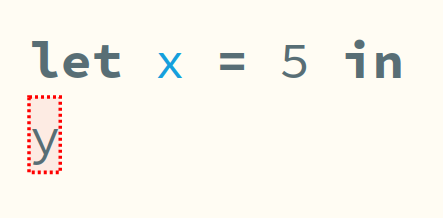
\includegraphics[width=\columnwidth]{images/haz3l-unbound-variable.png}
      \caption{Unbound variable error.}
      \label{fig:calculus-examples-unbound}
    \end{subfigure}
    &
    \begin{subfigure}[b]{0.3\columnwidth}
      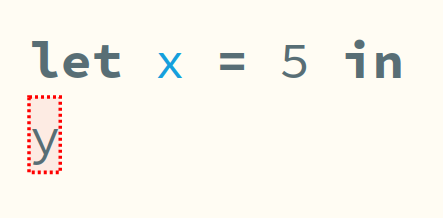
\includegraphics[width=\columnwidth]{images/haz3l-unbound-variable.png}
      \caption{Inconsistent types error.}
      \label{fig:calculus-examples-inconsistent-types}
    \end{subfigure} \\
    \begin{subfigure}[b]{0.3\columnwidth}
      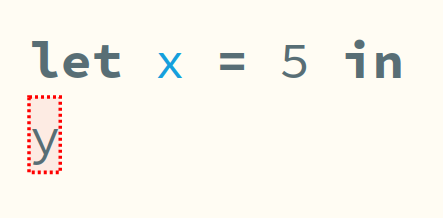
\includegraphics[width=\columnwidth]{images/haz3l-unbound-variable.png}
      \caption{Application of a non-lambda.}
      \label{fig:calculus-examples-app-non-lambda}
    \end{subfigure}
    &
    \begin{subfigure}[b]{0.3\columnwidth}
      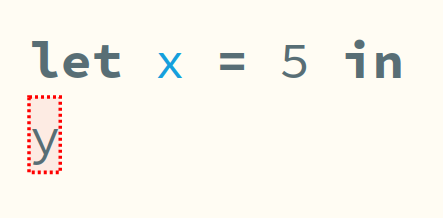
\includegraphics[width=\columnwidth]{images/haz3l-unbound-variable.png}
      \caption{Inconsistent branches error.}
      \label{fig:calculus-examples-inconsistent-branches}
    \end{subfigure}
  \end{tabular}
  %
  \caption{Examples of common type errors.}
  \label{fig:calculus-examples}
\end{figure}


Sometimes, the type an expression \emph{should} be is known. Consider
\cref{fig:calculus-examples-inconsistent-types}, in which it is expected that both operands of the
$+$ operator are numbers. Since $\textsf{true}$ is not a number, a type error arises, and Hazel
indicates a mismatch between the expected and actual types of the operand. The application in
\cref{fig:calculus-examples-app-non-lambda} of a non-lambda leads to a similar kind of error. In
this case, however, the expectation is not a singular type, but any member of a family of function
types. \Cref{fig:calculus-examples-inconsistent-branches} presents an error of inconsistent
branches: the branches of the if-else expression are of different types. Hazel opts to highlight the
entire expression in such a situation, while other tools may choose one branch to be ``correct'' and
``blame'' the type mismatch error on the other.

% TODO elaborate on this part

Unfortunately, formal typing semantics usually only give meaning to well-typed programs, leaving
such ill-typed ones meaningless. This is insufficient for editor services and language servers,
which must provide users feedback on where and why a program is ill-typed. Moreover, they must
continue providing semantic services even when an error is encountered. Indeed, similarly to
error-recovering parsers, real-world type checkers must robustly recover from type errors.
Traditionally, this has been performed in an \emph{ad hoc} manner [citations?], with different
languages and tools adopting varying approaches in the localization, reportage, and recovery of
errors.

% TODO examples of this ad hoc stuff

The key contribution of this section is the \emph{marked lambda calculus}, a formal calculus for
type error localization in bidirectional systems. Namely, the calculus provides a judgmental
framework with a unified theory for the design of typing semantics that support ill-typed programs.
\Cref{sec:calculus-calculus} describes its form and metatheory by example on a small gradually typed
lambda calculus, extending it with binary product types in \cref{sec:calculus-products}. All rules
and theorems may be found in the supplementary appendix, alongside a complete mechanization in the
Agda proof assistant, which is discussed briefly in \cref{sec:calculus-agda}. With products, we then
consider how error localization is complicated by patterned let expressions in
\cref{sec:calculus-let}. Finally, \cref{sec:calculus-poly} explores how the system might be extended
to more complex typing features, such as System F-style polymorphism.

% TODO not really sure when to start talking about bidirectional typing

% \emph{Bidirectional typing} combines type checking, which determines if a program satisfies a given
% type, and type synthesis, which generates a type from the program. This gives a simple algorithmic
% system in which type information is recursively propagated through terms and allows for local type
% inference.

% TODO talk about idea that bidirectional typing makes error localization easy? i.e. why choose
% bidirectional?

\subsection{The Calculus}
\label{sec:calculus-calculus}

% TODO outline the structure of this section at the beginning
% TODO make it clear unmarked/marked languages share same types

We now formally introduce the marked lambda calculus through its application to a gradually typed
lambda calculus extended with numbers and booleans. Consider the syntax for such a language, given
as $\EMName$ in \cref{fig:calculus-syntax}. The base types $\TNum$ and $\TBool$ classify number and
boolean expressions. The number literal corresponding to the mathematical number $n$ is given by
$\ENumMV$, and there is a single addition operation on numeric expressions. $\ETrue$ and $\EFalse$
correspond to the boolean values $\textsf{true}$ and $\textsf{false}$, respectively, and
$\EIf{\EMV_1}{\EMV_2}{\EMV_3}$ gives a conditional structure. In addition to these forms,
$\TUnknown$ is the unknown type from gradual type theory. $\EEHole$ denotes an \emph{expression
hole}, which are used to model syntactically incomplete programs---but are not critical within the
calculus.

\begin{figure}[htbp]
  \[\begin{array}{rrcl}
    \TMName  & \TMV  & \Coloneqq & \TUnknown \mid \TNum \mid \TBool \mid \TArrow{\TMV}{\TMV} \\
    \EMName  & \EMV  & \Coloneqq & x \mid \ELam{x}{\TMV}{\EMV} \mid \EAp{\EMV}{\EMV}
                       \mid           \ENumMV \mid \EPlus{\EMV}{\EMV}
                       \mid           \ETrue \mid \EFalse \mid \EIf{\EMV}{\EMV}{\EMV}
                       \mid           \EEHole \\
    \ECMName & \ECMV & \Coloneqq & x \mid \ECLam{x}{\TMV}{\ECMV} \mid \ECAp{\ECMV}{\ECMV}
                       \mid           \ECNumMV \mid \ECPlus{\ECMV}{\ECMV}
                       \mid           \ECTrue \mid \ECFalse \mid \ECIf{\ECMV}{\ECMV}{\ECMV}
                       \mid           \EEHole \\
             &       & \mid         & \ECUnbound{x} \mid \ECInconType{\ECMV} \mid \ECInconBr{\ECMV}{\ECMV}{\ECMV}
  \end{array}\]
  \caption{Syntax of an extended gradually typed lambda calculus.}
  \label{fig:calculus-syntax}
\end{figure}

Types classify expressions by a \emph{bidirectional type system}, which employs two mutually defined
judgments. \emph{Type synthesis}, written $\ctxSynType{\ctx}{\EMV}{\TMV}$, establishes that, under
the typing context $\ctx$, the expression $e$ synthesizes or infers the type $\TMV$. \emph{Type
analysis}, written $\ctxAnaType{\ctx}{\EMV}{\TMV}$, states that the expression $\EMV$ may appear
where an expression of type $\TMV$ is expected. We may give these typing semantics traditionally,
without considering error localization and recovery.

The marked lambda calculus builds atop these typing semantics into a two-layer system:
%
\begin{itemize}
  \item The \textbf{unmarked language}, which is the original language. Expressions of this language
    are called \emph{unmarked expressions}, denoted by the metavariable $\EMV$.

  \item The \textbf{marked language}, which mirrors the structure of the unmarked language but is
    extended with explicit \emph{error marks}. We call expressions of this language to be
    \emph{marked expressions}, denoted $\ECMV$.
    % TODO more intuition for what marked expressions are?

  \item \textbf{Marking}, which \emph{marks}, i.e. type checks and localizes errors for, any unmarked
    expression into a marked expression, inserting error marks where appropriate.
\end{itemize}
%
In other words, we extend the ordinary typing semantics of a language with a secondary ``marked''
language and ``mark'' unmarked programs into marked ones. This corresponds to a type checking
process with error localization and recovery. The marked language may then serve as a foundation for
other semantic services. % such as THI.

% TODO more intuition

\Cref{fig:calculus-syntax} furthermore gives the syntax for marked expressions (as $\ECMName$),
which replicates all the forms of unmarked expressions. There are additionally three kinds of
\emph{error marks}, which represent the different type errors that may arise.
%
\begin{itemize}
  \item $\ECUnbound{x}$, the \emph{unbound variable mark}, indicates the use of an unbound variable
    $x$, as in \cref{fig:calculus-examples-unbound}.

  \item $\ECInconType{\ECMV}$, the \emph{inconsistent type mark}, indicates that the type of an
    expression does not match an expected type.

  \item $\ECInconBr{\ECMV_1}{\ECMV_2}{\ECMV_3}$, the \emph{inconsistent branches mark}, indicates
    that the branches of a conditional have inconsistent types.
\end{itemize}
%
Throughout the remainder of this section, as we consider the formulation of marking, we will
motivate and give precise semantics for these error marks. Note that this is a non-exhaustive list;
depending on the syntactic forms and typing features found in the language, other kinds of marks may
be necessary. Indeed, in \cref{sec:calculus-poly}, we consider the kinds of marks that may be
required in an language with explicit polymorphism.

The marked language possesses its own typing semantics, also formulated bidirectionally. We write
$\ctxSynType{\ctx}{\ECMV}{\TMV}$ for synthesis and $\ctxAnaType{\ctx}{\ECMV}{\TMV}$ for analysis.
Finally, marking is bidirectional as well. The synthetic marking judgment
$\ctxSynFixedInto{\ctx}{\EMV}{\ECMV}{\TMV}$ establishes that, under the context $\Gamma$, the
unmarked expression $\EMV$ is ``marked into'' the marked expression $\ECMV$, which synthesizes type
$\TMV$. Analogously, the analytic marking judgment $\ctxAnaFixedInto{\ctx}{\EMV}{\ECMV}{\TMV}$
states that $\EMV$ is marked into $\ECMV$, which analyzes against $\TMV$.

How can we ensure that the marking procedure is correctly defined? There are two critical
metatheorems to keep in mind as we continue. The first is a \emph{totality} of marking:
%
\begin{theorem}[name=Marking Totality] \
  \label{thm:calculus-marking-totality}
  \begin{enumerate}
    \item For all $\ctx$ and $\EMV$, there exist $\ECMV$ and $\TMV$ such that
      $\ctxSynFixedInto{\ctx}{\EMV}{\ECMV}{\TMV}$.
  \item For all $\ctx$, $\EMV$, and $\TMV$, there exists $\ECMV$ such that
    $\ctxAnaFixedInto{\ctx}{\EMV}{\ECMV}{\TMV}$.
  \end{enumerate}
\end{theorem}
%
That is, we may mark \emph{any} syntactically well-formed program.

Furthermore, marking should preserve the syntactic structure of programs, modulo error marks. Thus,
we define a notion of \emph{mark erasure}, whose definition is given
\cref{fig:calculus-mark-erasure}, which converts marked expressions back into unmarked expression by
removing error marks. Then, \cref{thm:calculus-marking-well-formedness} provides a
\emph{well-formedness} criterion marking.
%
\begin{theorem}[name=Marking Well-Formedness] \
  \label{thm:calculus-marking-well-formedness}
  \begin{enumerate}
    \item If $\ctxSynFixedInto{\ctx}{\EMV}{\ECMV}{\TMV}$, then $\ctxSynType{\ctx}{\ECMV}{\TMV}$ and
      $\erasesTo{\ECMV}{\EMV}$.
    \item If $\ctxAnaFixedInto{\ctx}{\EMV}{\ECMV}{\TMV}$, then $\ctxAnaType{\ctx}{\ECMV}{\TMV}$ and
      $\erasesTo{\ECMV}{\EMV}$.
  \end{enumerate}
  % TODO split this into two theorems?
  % TODO not really sure how to intuitively describe the part about types matching up
\end{theorem}
%
In other words, if an unmarked expression is marked into some marked expression, erasing error marks
from the marked expression gives the original unmarked expression. We also ensure that marking gives
well-typed marked expressions; indeed, their types should match the types synthesized or analyzed
against in marking. % TODO more intuition for this theorem

\begin{figure}[htbp]
  \newcommand{\erasesToRow}[2]{\erase{#1} & = & #2}
  \[\begin{array}{rcl}
    % \erasesToRow{\ECEHole}{\EEHole} \\
    \erasesToRow{x}{x} \\
    \erasesToRow{(\ECLam{x}{\TMV}{\ECMV})}{\ELam{x}{\TMV}{(\erase{\ECMV})}} \\
    \erasesToRow{(\ECAp{\ECMV_1}{\ECMV_2})}{\EAp{(\erase{\ECMV_1})}{(\erase{\ECMV_2})}} \\
    % \erasesToRow{(\ECLet{x}{\ECMV_1}{\ECMV_2})}{\ELet{x}{(\erase{\ECMV_1})}{(\erase{\ECMV_2})}} \\
    \erasesToRow{\ECNumMV}{\ENumMV} \\
    \erasesToRow{(\ECPlus{\ECMV_1}{\ECMV_2})}{\EPlus{(\erase{\ECMV_1})}{(\erase{\ECMV_2})}} \\
    \erasesToRow{\ECTrue}{\ETrue} \\
    \erasesToRow{\ECFalse}{\EFalse} \\
    \erasesToRow{(\ECIf{\ECMV_1}{\ECMV_2}{\ECMV_3})}{\EIf{(\erase{\ECMV_1})}{(\erase{\ECMV_2})}{(\erase{\ECMV_3})}} \\
    \erasesToRow{\ECUnbound{x}}{x} \\
    \erasesToRow{\ECInconType{\ECMV}}{\erase{\ECMV}} \\
    \erasesToRow{\ECInconBr{\ECMV_1}{\ECMV_2}{\ECMV_3}}{\EIf{(\erase{\ECMV_1})}{(\erase{\ECMV_2})}{(\erase{\ECMV_3})}} \\
  \end{array}\]
  %
  \caption{Mark erasure definition.}
  \label{fig:calculus-mark-erasure}
\end{figure}


In the remainder of this subsection, we consider the different type errors that may arise in the
unmarked language; in this way, the typing semantics of the unmarked language guide the construction
of the marking process.

\subsubsection{Numbers}
\label{sec:calculus-numbers}

% TODO need to say something about subsumption and how it will be handled later.
To start, let us consider the simple case of numbers. Because of subsumption, we need only define a
synthesis rule for unmarked numbers, in which numbers synthesize the type $\TNum$:
%
\begin{mathpar}
  \judgment{ }{
    \ctxSynType{\ctx}{\ENumMV}{\TNum}
  }{USNum}
\end{mathpar}

Into what should numbers be marked? Quite straightforwardly, we simply give the same number as a
marked expression, synthesizing again $\TNum$. No type errors may occur in a single number, so we
only need the following rules for marking unmarked numbers and typing marked numbers:
%
\begin{mathpar}
  \judgment{
  }{
    \ctxSynFixedInto{\ctx}{\ENumMV}{\ECNumMV}{\TNum}
  }{MKSNum}

  \judgment{ }{
    \ctxSynType{\ctx}{\ECNumMV}{\TNum}
  }{MSNum}
\end{mathpar}

In addition expressions, the type of both operands should be $\TNum$. In a bidirectional system, we
thus analyze the operands against $\TNum$, giving the following rule:
%
\begin{mathpar}
  \judgment{
    \ctxAnaType{\ctx}{\EMV_1}{\TNum} \\
    \ctxAnaType{\ctx}{\EMV_2}{\TNum}
  }{
    \ctxSynType{\ctx}{\EPlus{\EMV_1}{\EMV_2}}{\TNum}
  }{USPlus}
\end{mathpar}

The marking rule mirrors \textsc{USPlus} closely. Since a known, expected type for each operand is
known, we shift the ``blame'' for any type errors to them. Hence, we recursively mark each operand
in analytic mode and rebuild the marked addition expression. The marked typing rule then mirrors
\textsc{USPlus} exactly.
%
\begin{mathpar}
  \judgment{
    \ctxAnaFixedInto{\ctx}{\EMV_1}{\ECMV_1}{\TNum} \\\\
    \ctxAnaFixedInto{\ctx}{\EMV_2}{\ECMV_2}{\TNum}
  }{
    \ctxSynFixedInto{\ctx}{\EPlus{\EMV_1}{\EMV_2}}{\ECPlus{\ECMV_1}{\ECMV_2}}{\TNum}
  }{MKSPlus}

  \judgment{
    \ctxAnaType{\ctx}{\ECMV_1}{\TNum} \\\\
    \ctxAnaType{\ctx}{\ECMV_2}{\TNum}
  }{
    \ctxSynType{\ctx}{\ECPlus{\ECMV_1}{\ECMV_2}}{\TNum}
  }{MSPlus}
\end{mathpar}

\subsubsection{Variables}
\label{sec:calculus-variables}

Let us now consider the more interesting case of variables. The typing of unmarked variables in the
gradually typed lambda calculus is standard. Again, because of subsumption, there is only a
synthetic rule:
\[%
  \judgment{
    \inCtx{\ctx}{x}{\TMV}
  }{
    \ctxSynType{\ctx}{x}{\TMV}
  }{USVar}
\]%
If $x$ is bound to a type in the typing context, it synthesizes that type. Straightforwardly,
marking converts the unmarked $x$ into the same marked $x$ via the following marking and typing
rules:
%
\begin{mathpar}
  \judgment{
    \inCtx{\ctx}{x}{\TMV}
  }{
    \ctxSynFixedInto{\ctx}{x}{x}{\TMV}
  }{MKSVar}

  \judgment{
    \inCtx{\ctx}{x}{\TMV}
  }{
    \ctxSynType{\ctx}{x}{\TMV}
  }{MSVar}
\end{mathpar}
% TODO more intuition on why this makes sense?

But what happens a variable, such as $y$ in \cref{fig:calculus-examples-unbound}, is \emph{not}
bound, i.e. that the premise fails? Then, \textsc{USVar} does not apply, and the typing semantics
say nothing about such expressions. When devising marking, to satisfy totality, such a possibility
motivates an \emph{unbound variable mark} $\ECUnbound{x}$, accompanied by the following rules:
%
\begin{mathpar}
  \judgment{
    \notInCtx{\ctx}{x}
  }{
    \ctxSynFixedInto{\ctx}{x}{\ECUnbound{x}}{\TUnknown}
  }{MKSUnbound}

  \judgment{
    \notInCtx{\ctx}{x}
  }{
    \ctxSynType{\ctx}{\ECUnbound{x}}{\TUnknown}
  }{MSUnbound}
\end{mathpar}
%
\textsc{MKSUnbound} states that an variable unbound in the context is marked into that variable
inside an unbound variable mark. \textsc{MSUnbound} then gives the typing of unbound variable marks.
Since nothing may be said about their types, we synthesize the unknown type, which allows type
checking to continue---instead of simply failing---and the unbound variable to be used in any
expression. % TODO clarify why this is correct

\subsubsection{Lambda Abstractions}
\label{sec:calculus-lambda-abstractions}

There are explicit synthesis and analysis rules for unmarked lambda abstractions:
%
\begin{mathpar}
  \judgment{
    \ctxSynType{\extendCtx{\ctx}{x}{\TMV}}{\EMV}{\TMV_2}
  }{
    \ctxSynType{\ctx}{\ELam{x}{\TMV_1}{\EMV}}{\TArrow{\TMV_1}{\TMV_2}}
  }{USLam}

  \judgment{
    \matchedArrow{\TMV_3}{\TMV_1}{\TMV_2} \\
    \consistent{\TMV}{\TMV_1} \\
    \ctxAnaType{\extendCtx{\ctx}{x}{\TMV}}{\EMV}{\TMV_2}
  }{
    \ctxAnaType{\ctx}{\ECLam{x}{\TMV}{\EMV}}{\TMV_3}
  }{UALam}
\end{mathpar}
%
The synthesis rule is standard. In the premises of \textsc{UALam}, we use the notion of
\emph{type consistency} from gradual type theory, which defines a reflexive and symmetric (but not
transitive) relation between types, writing $\consistent{\TMV_1}{\TMV_2}$ to mean that $\TMV_1$ is
consistent with $\TMV_2$. This replaces the notion of \emph{type equality} to relate the unknown
type to all other types. The analysis rule also employs the judgment
$\matchedArrow{\TMV}{\TMV_1}{\TMV_2}$, which establishes that $\TMV$ is a \emph{matched arrow type},
i.e. it may be considered an arrow type. This notion is purely a technical mechanism to avoid
duplication of rules related to arrow types. \Cref{fig:calculus-consistency-matched-arrow} gives the
rules for both judgments.

% TODO mention explicitly that by inductive hypothesis, the marking of body cannot fail?
% TODO more intuition on these two judgments
% TODO more intuition on USLam and UALam

\begin{figure}[htbp]
  \raggedright
  \judgbox{\ensuremath{\consistent{\TMV_1}{\TMV_2}}} $\TMV_1$ is consistent with $\TMV_2$
  %
  \begin{mathpar}
    \judgment{ }{
      \consistent{\TUnknown}{\TMV}
    }{TCUnknown1}

    \judgment{ }{
      \consistent{\TMV}{\TUnknown}
    }{TCUnknown2}

    \judgment{ }{
      \consistent{\TMV}{\TMV}
    }{TCRefl}

    \judgment{
      \consistent{\TMV_1}{\TMV_1'} \\
      \consistent{\TMV_2}{\TMV_2'} \\
    }{
      \consistent{\TArrow{\TMV_1}{\TMV_2}}{\TArrow{\TMV_1'}{\TMV_2'}}
    }{TCArr} \\
  \end{mathpar}

  \judgbox{\ensuremath{\matchedArrow{\TMV}{\TMV_1}{\TMV_2}}} $\TMV$ has matched arrow type $\TArrow{\TMV_1}{\TMV_2}$
  %
  \begin{mathpar}
    \judgment{ }{
      \matchedArrow{\TUnknown}{\TUnknown}{\TUnknown}
    }{TMAHole}

    \judgment{ }{
      \matchedArrow{\TArrow{\TMV}{\TMV}}{\TMV}{\TMV}
    }{TMAArr}
  \end{mathpar}
  %
  \caption{Type consistency and matched arrow types.}
  \label{fig:calculus-consistency-matched-arrow}
\end{figure}

The synthesis rule for marking intuitively follows \textsc{USLam} closely. We should recursively
mark the body with an extended context binding $x$ to $\TMV$ and construct a new marked lambda
abstraction:
%
\begin{mathpar}
  \judgment{
    \ctxSynFixedInto{\extendCtx{\ctx}{x}{\TMV_1}}{\EMV}{\ECMV}{\TMV_2}
  }{
    \ctxSynFixedInto{\ctx}{\ELam{x}{\TMV_1}{\EMV}}{\ELam{x}{\TMV_1}{\ECMV}}{\TArrow{\TMV_1}{\TMV_2}}
  }{MKSLam}

  \judgment{
    \ctxSynType{\extendCtx{\ctx}{x}{\TMV}}{\ECMV}{\TMV_2}
  }{
    \ctxSynType{\ctx}{\ECLam{x}{\TMV_1}{\ECMV}}{\TArrow{\TMV_1}{\TMV_2}}
  }{MSLam}
\end{mathpar}
%
Similarly, we construct corresponding analytic rules:
%
\begin{mathpar}
  \judgment{
    \matchedArrow{\TMV_3}{\TMV_1}{\TMV_2} \\
    \consistent{\TMV}{\TMV_1} \\\\
    \ctxAnaFixedInto{\extendCtx{\ctx}{x}{\TMV}}{\EMV}{\ECMV}{\TMV_2}
  }{
    \ctxAnaFixedInto{\ctx}{\ELam{x}{\TMV}{\EMV}}{\ECLam{x}{\TMV}{\ECMV}}{\TMV_3}
  }{MKALam1}

  \judgment{
    \matchedArrow{\TMV_3}{\TMV_1}{\TMV_2} \\
    \consistent{\TMV}{\TMV_1} \\\\
    \ctxAnaType{\extendCtx{\ctx}{x}{\TMV}}{\ECMV}{\TMV_2}
  }{
    \ctxAnaType{\ctx}{\ECLam{x}{\TMV}{\ECMV}}{\TMV_3}
  }{MALam1}
\end{mathpar}
%
However, recalling totality, we look again to the premises of \textsc{UALam} to see what type errors
may arise. First, what if $\TMV_3$ is not a matched arrow type? This would be the case if it were
$\TNum$, for example, and the lambda abstraction would be inconsistent with the expected type. Thus,
to the syntax we add an \emph{inconsistent type mark} $\ECInconType{\ECMV}$, which indicates that
the expression does not synthesize a type consistent with the expected type. We then have the
following rules, in which the lambda abstraction is placed inside the inconsistent type mark.
%
\begin{mathpar}
  \judgment{
    \notMatchedArrow{\TMV_3} \\
    \ctxAnaFixedInto{\extendCtx{\ctx}{x}{\TMV}}{\EMV}{\ECMV}{\TUnknown}
  }{
    \ctxAnaFixedInto{\ctx}{\ELam{x}{\TMV}{\EMV}}{\ECInconType{\ECLam{x}{\TMV}{\ECMV}}}{\TMV_3}
  }{MKALam2}

  \judgment{
    \notMatchedArrow{\TMV_3} \\
    \ctxAnaType{\extendCtx{\ctx}{x}{\TMV}}{\ECMV}{\TUnknown}
  }{
    \ctxAnaType{\ctx}{\ECInconType{\ECLam{x}{\TMV}{\ECMV}}}{\TMV_3}
  }{MALam2}
\end{mathpar}
%
Though no expected output type is known, we still need to check and mark the body; it is thus
analyzed against the unknown type in \textsc{MKALam2}.

A similar situation arises when $\matchedArrow{\TMV_3}{\TMV_1}{\TMV_2}$, but
$\inconsistent{\TMV}{\TMV_1}$, i.e. the expected input type is inconsistent with the actual input
type, giving the last pair of analytic rules for lambda abstractions:
%
\begin{mathpar}
  \judgment{
    \matchedArrow{\TMV_3}{\TMV_1}{\TMV_2} \\
    \inconsistent{\TMV}{\TMV_1} \\\\
    \ctxAnaFixedInto{\extendCtx{\ctx}{x}{\TMV}}{\EMV}{\ECMV}{\TMV_2}
  }{
    \ctxAnaFixedInto{\ctx}{\ELam{x}{\TMV}{\EMV}}{\ECInconType{\ECLam{x}{\TMV}{\ECMV}}}{\TMV_3}
  }{MKALam3}

  \judgment{
    \matchedArrow{\TMV_3}{\TMV_1}{\TMV_2} \\
    \inconsistent{\TMV}{\TMV_1} \\\\
    \ctxAnaType{\extendCtx{\ctx}{x}{\TMV}}{\ECMV}{\TMV_2}
  }{
    \ctxAnaType{\ctx}{\ECInconType{\ECLam{x}{\TMV}{\ECMV}}}{\TMV_3}
  }{MALam3}
\end{mathpar}

\subsubsection{Applications}
\label{sec:calculus-applications}

The case of application is somewhat interesting. In the unmarked language, only a synthesis rule is
necessary:
\[%
  \judgment{
    \ctxSynType{\ctx}{\EMV_1}{\TMV} \\
    \matchedArrow{\TMV}{\TMV_1}{\TMV_2} \\
    \ctxAnaType{\ctx}{\EMV_2}{\TMV_1}
  }{
    \ctxSynType{\ctx}{\EAp{\EMV_1}{\EMV_2}}{\TMV_2}
  }{USAp}
\]%
Following the same methodology, we can straightforwardly give the following marking and typing
rules:
%
\begin{mathpar}
  \judgment{
    \ctxSynFixedInto{\ctx}{\EMV_1}{\ECMV_1}{\TMV} \\
    \matchedArrow{\TMV}{\TMV_1}{\TMV_2} \\\\
    \ctxAnaFixedInto{\ctx}{\EMV_2}{\ECMV_2}{\TMV_1} \\
  }{
    \ctxSynFixedInto{\ctx}{\EAp{\EMV_1}{\EMV_2}}{\ECAp{\ECMV_1}{\ECMV_2}}{\TMV_2}
  }{MKSAp1}

  \judgment{
    \ctxSynType{\ctx}{\ECMV_1}{\TMV} \\
    \matchedArrow{\TMV}{\TMV_1}{\TMV_2} \\\\
    \ctxAnaType{\ctx}{\ECMV_2}{\TMV_1}
  }{
    \ctxSynType{\ctx}{\ECAp{\ECMV_1}{\ECMV_2}}{\TMV_2}
  }{MSAp1}
\end{mathpar}

Again, to satisfy totality, we must consider the case when $\TMV$ is not a matched arrow type, such
as in the example of \cref{fig:calculus-examples-app-non-lambda}. There is no expected type for the
argument, so we perform analytic marking on $\EMV_2$ against the unknown type. The applied
expression is placed inside the inconsistent type mark, which is in accordance with the meaning of
that mark.
%
\begin{mathpar}
  \judgment{
    \ctxSynFixedInto{\ctx}{\EMV_1}{\ECMV_1}{\TMV} \\
    \notMatchedArrow{\TMV} \\\\
    \ctxAnaFixedInto{\ctx}{\EMV_2}{\ECMV_2}{\TUnknown}
  }{
    \ctxSynFixedInto{\ctx}{\EAp{\EMV_1}{\EMV_2}}{\ECApNonMatched{\ECMV_1}{\ECMV_2}}{\TUnknown}
  }{MKSAp2}

  \judgment{
    \ctxSynType{\ctx}{\ECMV_1}{\TMV} \\
    \notMatchedArrow{\TMV} \\\\
    \ctxAnaType{\ctx}{\ECMV_2}{\TUnknown}
  }{
    \ctxSynType{\ctx}{\ECApNonMatched{\ECMV_1}{\ECMV_2}}{\TUnknown}
  }{MSAp2}
\end{mathpar}

It is worth noting, however, that $\EMV_1$ is not actually in analytic position, but in a synthetic
position where any arrow type is expected. Treating such ``constrained synthetic'' cases specially,
we may instead designate a specialized mark, written $\ECApNonMatchedAltAlt{\ECMV}$. This yields the
following alternative rules:
%
\[\begin{array}{rrcl}
  \ECMName & \ECMV & \Coloneqq & \cdots \mid \ECApNonMatchedAltAlt{\ECMV}
\end{array}\]
%
\begin{mathpar}
  \judgment{
    \ctxSynFixedInto{\ctx}{\EMV_1}{\ECMV_1}{\TMV} \\
    \notMatchedArrow{\TMV} \\\\
    \ctxAnaFixedInto{\ctx}{\EMV_2}{\ECMV_2}{\TUnknown}
  }{
    \ctxSynFixedInto{\ctx}{\EAp{\EMV_1}{\EMV_2}}{\ECAp{\ECApNonMatchedAltAlt{\ECMV_1}}{\ECMV_2}}{\TUnknown}
  }{MKSAp2'}

  \judgment{
    \ctxSynType{\ctx}{\ECMV_1}{\TMV} \\
    \notMatchedArrow{\TMV} \\\\
    \ctxAnaType{\ctx}{\ECMV_2}{\TUnknown}
  }{
    \ctxSynType{\ctx}{\ECApNonMatchedAltAlt{\ECMV_1}{\ECMV_2}}{\TUnknown}
  }{MSAp2'}
\end{mathpar}

It is natural to extend this approach to other elimination forms that require the handling of
unmatched types, such as products. Another approach is to mark an error around the entire
application expression.

\subsubsection{Booleans}
\label{sec:calculus-booleans}

Boolean values are similarly straightforward:
%
\begin{mathpar}
  \judgment{ }{
    \ctxSynType{\ctx}{\ETrue}{\TBool}
  }{USTrue}

  \judgment{
  }{
    \ctxSynFixedInto{\ctx}{\ETrue}{\ECTrue}{\TBool}
  }{MKSTrue}

  \judgment{ }{
    \ctxSynType{\ctx}{\ECTrue}{\TBool}
  }{MSTrue} \\

  \judgment{ }{
    \ctxSynType{\ctx}{\EFalse}{\TBool}
  }{USFalse}

  \judgment{
  }{
    \ctxSynFixedInto{\ctx}{\EFalse}{\ECFalse}{\TBool}
  }{MKSFalse}

  \judgment{ }{
    \ctxSynType{\ctx}{\ECFalse}{\TBool}
  }{MSFalse}
\end{mathpar}

If-else expressions, however, offer another interesting case. In the unmarked language, we have
both explicit synthetic and analytic rules:
%
\begin{mathpar}
  \judgment{
    \ctxAnaType{\ctx}{\EMV_1}{\TBool} \\\\
    \ctxSynType{\ctx}{\EMV_2}{\TMV_1} \\
    \ctxSynType{\ctx}{\EMV_3}{\TMV_2}
  }{
    \ctxSynType{\ctx}{\EIf{\EMV_1}{\EMV_2}{\EMV_3}}{\TJoin{\TMV_1}{\TMV_2}}
  }{USIf}

  \judgment{
    \ctxAnaType{\ctx}{\EMV_1}{\TBool} \\\\
    \ctxAnaType{\ctx}{\EMV_1}{\TMV} \\
    \ctxAnaType{\ctx}{\EMV_2}{\TMV}
  }{
    \ctxAnaType{\ctx}{\ECIf{\EMV_1}{\EMV_2}{\EMV_3}}{\TMV}
  }{UAIf}
\end{mathpar}
%
In synthetic position, conditionals synthesize the \emph{join} of the branch types $\TMV_1$ and
$\TMV_2$, which we define inductively in \cref{fig:calculus-type-join}. In analytic position, since
there is an expected type for both branches, we shift the blame for any errors to them.

% TODO intuition why we use join

\newcommand{\joinsTo}[3]{\ensuremath{\TJoin{#1}{#2} & = & #3}}
\begin{figure}[htbp]
  \raggedright
  \judgbox{\ensuremath{\TJoin{\TMV_1}{\TMV_2}}} is a \emph{partial} metafunction defined as follows:
  %
  \[\begin{array}{rcl}
    \joinsTo{\TUnknown}{\TMV}{\TMV} \\
    \joinsTo{\TMV}{\TUnknown}{\TMV} \\
    \joinsTo{\TNum}{\TNum}{\TNum} \\
    \joinsTo{\TBool}{\TBool}{\TBool} \\
    \joinsTo{(\TArrow{\TMV_1}{\TMV_2})}{(\TArrow{\TMV_1'}{\TMV_2'})}{\TArrow{(\TJoin{\TMV_1}{\TMV_1'})}{(\TJoin{\TMV_2}{\TMV_2'})}} \\
  \end{array}\]
  %
  \caption{Type join.}
  \label{fig:calculus-type-join}
\end{figure}
% TODO intuition for type join?

Following \textsc{USIf} and \textsc{UAIf}, we may derive the following marking and typing rules.
Similar to previous cases, we simply recursively mark the guard and branch expressions and construct
the marked conditional from the results.
%
\begin{mathpar}
  \judgment{
    \ctxAnaFixedInto{\ctx}{\EMV_1}{\ECMV_1}{\TBool} \\\\
    \ctxSynFixedInto{\ctx}{\EMV_2}{\ECMV_2}{\TMV_1} \\
    \ctxSynFixedInto{\ctx}{\EMV_3}{\ECMV_3}{\TMV_2}
  }{
    \ctxSynFixedInto{\ctx}{\EIf{\EMV_1}{\EMV_2}{\EMV_3}}{\ECIf{\ECMV_1}{\ECMV_2}{\ECMV_3}}{\TJoin{\TMV_1}{\TMV_2}}
  }{MKSIf}

  \judgment{
    \ctxAnaType{\ctx}{\ECMV_1}{\TBool} \\\\
    \ctxSynType{\ctx}{\ECMV_2}{\TMV_1} \\
    \ctxSynType{\ctx}{\ECMV_3}{\TMV_2}
  }{
    \ctxSynType{\ctx}{\ECIf{\ECMV_1}{\ECMV_2}{\ECMV_3}}{\TJoin{\TMV_1}{\TMV_2}}
  }{MSIf} \\

  \judgment{
    \ctxAnaFixedInto{\ctx}{\EMV_1}{\ECMV_1}{\TBool} \\\\
    \ctxAnaFixedInto{\ctx}{\EMV_2}{\ECMV_2}{\TMV} \\
    \ctxAnaFixedInto{\ctx}{\EMV_3}{\ECMV_3}{\TMV} \\
  }{
    \ctxAnaFixedInto{\ctx}{\EIf{\EMV_1}{\EMV_2}{\EMV_3}}{\ECIf{\ECMV_1}{\ECMV_2}{\ECMV_3}}{\TMV}
  }{MKAIf}

  \judgment{
    \ctxAnaType{\ctx}{\ECMV_1}{\TBool} \\\\
    \ctxAnaType{\ctx}{\ECMV_1}{\TMV} \\
    \ctxAnaType{\ctx}{\ECMV_2}{\TMV}
  }{
    \ctxAnaType{\ctx}{\ECIf{\ECMV_1}{\ECMV_2}{\ECMV_3}}{\TMV}
  }{MAIf}
\end{mathpar}

However, in synthetic mode, it may be the case that the two branch types have no join. This occurs,
in fact, when they are inconsistent. This motivates \emph{the inconsistent branches mark}
$\ECInconBr{\ECMV}{\ECMV}{\ECMV}$. Then, adding the following rules ensures marking totality on
conditionals:
%
\begin{mathpar}
  \judgment{
    \ctxAnaFixedInto{\ctx}{\EMV_1}{\ECMV_1}{\TBool} \\
    \ctxSynFixedInto{\ctx}{\EMV_2}{\ECMV_2}{\TMV_1} \\\\
    \ctxSynFixedInto{\ctx}{\EMV_3}{\ECMV_3}{\TMV_2} \\
    \inconsistent{\TMV_1}{\TMV_2}
  }{
    \ctxSynFixedInto{\ctx}{\EIf{\EMV_1}{\EMV_2}{\EMV_3}}{\ECInconBr{\ECMV_1}{\ECMV_2}{\ECMV_3}}{\TUnknown}
  }{MKSInconsistentBranches}

  \judgment{
    \ctxAnaType{\ctx}{\ECMV_1}{\TBool} \\
    \ctxSynType{\ctx}{\ECMV_2}{\TMV_1} \\\\
    \ctxSynType{\ctx}{\ECMV_3}{\TMV_2} \\
    \inconsistent{\TMV_1}{\TMV_2}
  }{
    \ctxSynType{\ctx}{\ECInconBr{\ECMV_1}{\ECMV_2}{\ECMV_3}}{\TUnknown}
  }{MSInconsistentBranches}
\end{mathpar}

\subsubsection{Subsumption}
\label{sec:calculus-subsumption}

Finally, we consider the subsumption rule in typing unmarked expressions, which states that if an
expression synthesizes a type, it may also be analyzed against that type or any consistent type.
\[%
  \judgment{
    \ctxSynType{\ctx}{\EMV}{\TMV'} \\
    \consistent{\TMV}{\TMV'} \\
    \subsumable{\EMV}
  }{
    \ctxAnaType{\ctx}{\EMV}{\TMV}
  }{UASubsume}
\]%
We also restrict the usage of subsumption to ``subsumable'' syntactic forms, written
$\subsumable{\EMV}$. This judgment is defined on all syntactic forms except lambda abstractions and
conditionals, the only ones with explicit analysis rules. In other words, we restrict
subsumption to be the analytic rule of ``last resort''. This is critical in establishing that
marking and typing are deterministic (discussed later in \cref{thm:calculus-marking-unicity}).

Since we did not provide explicit analytic rules for marking expressions that are not lambda
abstractions or conditionals (or typing their marked versions) either, we give corresponding
subsumption rules:
%
\begin{mathpar}
  \judgment{
    \ctxSynFixedInto{\ctx}{\EMV}{\ECMV}{\TMV'} \\
    \consistent{\TMV}{\TMV'} \\
    \subsumable{\EMV}
  }{
    \ctxAnaFixedInto{\ctx}{\EMV}{\ECMV}{\TMV}
  }{MKASubsume}

  \judgment{
    \ctxSynType{\ctx}{\ECMV}{\TMV'} \\
    \consistent{\TMV}{\TMV'} \\
    \subsumable{\ECMV}
  }{
    \ctxAnaType{\ctx}{\ECMV}{\TMV}
  }{MASubsume}
\end{mathpar}
%
Note that we define a analogous notion of ``subsumability'' for marked expressions, written
$\subsumable{\ECMV}$.

However, it may be the case that the expression is inconsistent with the expected type. Recalling
the example of \cref{fig:calculus-examples-inconsistent-types}, subsumption would used to analyze
$\ETrue$ against $\TNum$ in $\EPlus{\ETrue}{5}$, which fails since $\inconsistent{\TNum}{\TBool}$,
and $\ETrue$ should be marked with an inconsistent type mark. Hence, the following final set of
rules is required to handle such cases:
%
\begin{mathpar}
  \judgment{
    \ctxSynFixedInto{\ctx}{\EMV}{\ECMV}{\TMV'} \\
    \inconsistent{\TMV}{\TMV'} \\\\
    \subsumable{\EMV}
  }{
    \ctxAnaFixedInto{\ctx}{\EMV}{\ECInconType{\ECMV}}{\TMV}
  }{MKAInconsistentTypes}

  \judgment{
    \ctxSynType{\ctx}{\ECMV}{\TMV'} \\
    \inconsistent{\TMV}{\TMV'} \\\\
    \subsumable{\ECMV}
  }{
    \ctxAnaType{\ctx}{\ECInconType{\ECMV}}{\TMV}
  }{MAInconsistentTypes}
\end{mathpar}
%
These rules complete the development of the marked lambda calculus for the gradually typed lambda
calculus.

% TODO mini conclusion on methodology

To conclude this section, we present two more metatheorems that help ensure correctness of the
system. Though \cref{thm:calculus-marking-well-formedness} guarantees that marking does not change
the syntactic structure of a program, it makes no statement about the presence of error marks in the
resulting marked program. Following the logic of constructing marking rules, we have
\cref{thm:calculus-marking-well-ill-typed}.

\begin{theorem}[name=Marking of Well-Typed/Ill-Typed Expressions] \ % TODO better name for this
  \label{thm:calculus-marking-well-ill-typed}
  \begin{enumerate}
    \item \begin{enumerate}
        \item If $\ctxSynType{\ctx}{\EMV}{\TMV}$ and $\ctxSynFixedInto{\ctx}{\EMV}{\ECMV}{\TMV}$,
          then $\imageIs{\EMV}{\ECMV}$.
        \item If $\ctxAnaType{\ctx}{\EMV}{\TMV}$ and $\ctxAnaFixedInto{\ctx}{\EMV}{\ECMV}{\TMV}$,
          then $\imageIs{\EMV}{\ECMV}$.
      \end{enumerate}

    \item \begin{enumerate}
        \item If there does not exist $\TMV$ such that $\ctxSynType{\ctx}{\EMV}{\TMV}$, then for all
          $\ECMV$ and $\TMV'$ such that $\ctxSynFixedInto{\ctx}{\EMV}{\ECMV}{\TMV'}$, we have
          $\imageIsNot{\EMV}{\ECMV}$.
        \item If there does not exist $\TMV$ such that $\ctxAnaType{\ctx}{\EMV}{\TMV}$, then for all
          $\ECMV$ and $\TMV'$ such that $\ctxAnaFixedInto{\ctx}{\EMV}{\ECMV}{\TMV'}$, we have
          $\imageIsNot{\EMV}{\ECMV}$.
      \end{enumerate}
  \end{enumerate}
\end{theorem}
%
That is, since error marks indicate type errors in the program, no marks should be inserted
into a well-typed program. The converse---that at least one mark is inserted into ill-typed
programs---is also true. We have chosen to formulate the absence of error marks through an inclusion
mapping of unmarked expressions into marked expressions; alternatively, a predicate over marked
expressions may be used. % TODO latter is easier to do in Agda, but maybe it is weaker?

Finally, no less importantly, marking is deterministic. This is given by
\cref{thm:calculus-marking-unicity}.
%
\begin{theorem}[name=Marking Unicity] \
  \label{thm:calculus-marking-unicity}
  \begin{enumerate}
    \item If $\ctxSynFixedInto{\ctx}{\EMV}{\ECMV_1}{\TMV_1}$ and
      $\ctxSynFixedInto{\ctx}{\EMV}{\ECMV_2}{\TMV_2}$, then $\ECMV_1 = \ECMV_2$ and $\TMV_1 =
      \TMV_2$.
    \item If $\ctxAnaFixedInto{\ctx}{\EMV}{\ECMV_1}{\TMV}$ and
      $\ctxAnaFixedInto{\ctx}{\EMV}{\ECMV_2}{\TMV}$, then $\ECMV_1 = \ECMV_2$.
  \end{enumerate}
\end{theorem}
%
Together with totality, marking may be considered and implemented as a total function.

% TODO non-gradual semantics?

% Note that while the semantics that follow concern a gradually typed language, a non-gradual system
% may be recovered straightforwardly by removing the unknown type and replacing type consistency with
% equality.

\subsection{Adding Binary Products}
\label{sec:calculus-products}

We now demonstrate how one might extend or adapt the marked lambda calculus for new typing features
by adding binary product types. First, in \cref{fig:calculus-product-judgments}, we extend the
syntax of types and the accompanying notions of consistency and join, which closely mirror the
definitions for arrow types.
%
\[\begin{array}{rrcl}
  \TMName  & \TMV  & \Coloneqq & \cdots \mid \TPair{\TMV}{\TMV}
\end{array}\]

We additionally define an auxiliary notion of \emph{matched binary product types}: the judgment
$\matchedPair{\TMV}{\TMV_1}{\TMV_2}$ establishes that $\TMV$ may be considered the binary product
type $\TPair{\TMV_1}{\TMV_2}$.

\begin{figure}[htbp]
  \raggedright
  \judgbox{\ensuremath{\consistent{\TMV_1}{\TMV_2}}} $\TMV_1$ is consistent with $\TMV_2$
  %
  \begin{mathpar}
    \judgment{
      \consistent{\TMV_1}{\TMV_1'} \\
      \consistent{\TMV_2}{\TMV_2'} \\
    }{
      \consistent{\TPair{\TMV_1}{\TMV_2}}{\TPair{\TMV_1'}{\TMV_2'}}
    }{TCProd} \\
  \end{mathpar}

  \judgbox{\ensuremath{\TJoin{\TMV_1}{\TMV_2}}} is a \emph{partial} metafunction defined as follows:
  %
  \[\begin{array}{rcl}
    & \cdots & \\
    \joinsTo{(\TPair{\TMV_1}{\TMV_2})}{(\TPair{\TMV_1'}{\TMV_2'})}{\TPair{(\TJoin{\TMV_1}{\TMV_1'})}{(\TJoin{\TMV_2}{\TMV_2'})}} \\
  \end{array}\]

  \judgbox{\ensuremath{\matchedPair{\TMV}{\TMV_1}{\TMV_2}}} $\TMV$ has matched binary product type $\TPair{\TMV_1}{\TMV_2}$
  %
  \begin{mathpar}
    \judgment{ }{
      \matchedPair{\TUnknown}{\TUnknown}{\TUnknown}
    }{TMPHole}

    \judgment{ }{
      \matchedPair{\TPair{\TMV_1}{\TMV_2}}{\TMV_1}{\TMV_2}
    }{TMPProd}
  \end{mathpar}
  %
  \caption{Binary product consistency, join, and matched product type.}
  \label{fig:calculus-product-judgments}
\end{figure}

The unmarked language is extended with a pair constructor and projection operators. In addition to
the synthesis rules, we have explicit analysis rules. If an expected type is known for a pair
expression, the responsibility for type errors is given to the components. Likewise, we shift blame
to the projected expression when analysing projections.
%
\[\begin{array}{rrcl}
  \EMName  & \EMV  & \Coloneqq & \cdots
                               \mid \EPair{\EMV}{\EMV}
                               \mid \EProjL{\EMV} \mid \EProjR{\EMV}
\end{array}\]
%
\begin{mathpar}
  \judgment{
    \ctxSynType{\ctx}{\EMV_1}{\TMV_1} \\
    \ctxSynType{\ctx}{\EMV_2}{\TMV_2}
  }{
    \ctxSynType{\ctx}{\EPair{\EMV_1}{\EMV_2}}{\TPair{\TMV_1}{\TMV_2}}
  }{USPair}

  \judgment{
    \ctxSynType{\ctx}{\EMV}{\TMV} \\
    \matchedPair{\TMV}{\TMV_1}{\TMV_2}
  }{
    \ctxSynType{\ctx}{\EProjL{\EMV}}{\TMV_1}
  }{USProjL}

  \judgment{
    \ctxSynType{\ctx}{\EMV}{\TMV} \\
    \matchedPair{\TMV}{\TMV_1}{\TMV_2}
  }{
    \ctxSynType{\ctx}{\EProjR{\EMV}}{\TMV_2}
  }{USProjR} \\

  \judgment{
    \matchedPair{\TMV}{\TMV_1}{\TMV_2} \\
    \ctxAnaType{\ctx}{\EMV_1}{\TMV_1} \\
    \ctxAnaType{\ctx}{\EMV_2}{\TMV_2}
  }{
    \ctxAnaType{\ctx}{\EPair{\EMV_1}{\EMV_2}}{\TMV}
  }{UAPair}

  \judgment{
    \ctxAnaType{\ctx}{\EMV}{\TPair{\TMV}{\TUnknown}}
  }{
    \ctxAnaType{\ctx}{\EProjL{\EMV}}{\TMV}
  }{UAProjL}

  \judgment{
    \ctxAnaType{\ctx}{\EMV}{\TPair{\TUnknown}{\TMV}}
  }{
    \ctxAnaType{\ctx}{\EProjR{\EMV}}{\TMV}
  }{UAProjR}
\end{mathpar}
%
Similarly to application, \textsc{USProjL} and \textsc{USProjR} employ the matched binary product
type judgment; a projection $\EProjL{\EMV}$ or $\EProjR{\EMV}$ is then well-typed if the $\EMV$ may
be considered to be a pair.

The marked language is extended with the same forms, and we devise the following marking rules,
again modelling off the above unmarked typing rules:
%
\[\begin{array}{rrcl}
  \ECMName & \ECMV & \Coloneqq & \cdots
                               \mid \ECPair{\ECMV}{\ECMV}
                               \mid \ECProjL{\ECMV} \mid \ECProjR{\ECMV}
                               \mid \ECInconMatchedPair{\ECMV}
\end{array}\]
%
\begin{mathpar}
  \judgment{
    \ctxSynFixedInto{\ctx}{\EMV_1}{\ECMV_1}{\TMV_1} \\\\
    \ctxSynFixedInto{\ctx}{\EMV_2}{\ECMV_2}{\TMV_2}
  }{
    \ctxSynFixedInto{\ctx}{\EPair{\EMV_1}{\EMV_2}}{\ECPair{\ECMV_1}{\ECMV_2}}{\TPair{\TMV_1}{\TMV_2}}
  }{MKSPair}

  \judgment{
    \ctxSynFixedInto{\ctx}{\EMV}{\ECMV}{\TMV} \\\\
    \matchedPair{\TMV}{\TMV_1}{\TMV_2}
  }{
    \ctxSynFixedInto{\ctx}{\EProjL{\EMV}}{\ECProjL{\ECMV}}{\TMV_1}
  }{MKSProjL1}

  \judgment{
    \ctxSynFixedInto{\ctx}{\EMV}{\ECMV}{\TMV} \\\\
    \matchedPair{\TMV}{\TMV_1}{\TMV_2}
  }{
    \ctxSynFixedInto{\ctx}{\EProjR{\EMV}}{\ECProjR{\ECMV}}{\TMV_2}
  }{MKSProjR1} \\

  \judgment{
    \matchedPair{\TMV}{\TMV_1}{\TMV_2} \\
    \ctxAnaFixedInto{\ctx}{\EMV_1}{\ECMV_1}{\TMV_1} \\\\
    \ctxAnaFixedInto{\ctx}{\EMV_2}{\ECMV_2}{\TMV_2}
  }{
    \ctxAnaFixedInto{\ctx}{\EPair{\EMV_1}{\EMV_2}}{\ECPair{\ECMV_1}{\ECMV_2}}{\TMV}
  }{MKAPair1}

  \judgment{
    \ctxAnaFixedInto{\ctx}{\EMV}{\ECMV}{\TPair{\TMV}{\TUnknown}}
  }{
    \ctxAnaFixedInto{\ctx}{\EProjL{\EMV}}{\ECProjL{\ECMV}}{\TMV}
  }{MKAProjL}

  \judgment{
    \ctxAnaFixedInto{\ctx}{\EMV}{\ECMV}{\TPair{\TMV}{\TUnknown}}
  }{
    \ctxAnaFixedInto{\ctx}{\EProjR{\EMV}}{\ECProjR{\ECMV}}{\TMV}
  }{MKAProjR}
\end{mathpar}
%
accompanied by corresponding typing rules for marked expressions:
%
\begin{mathpar}
  \judgment{
    \ctxSynType{\ctx}{\ECMV_1}{\TMV_1} \\
    \ctxSynType{\ctx}{\ECMV_2}{\TMV_2}
  }{
    \ctxSynType{\ctx}{\ECPair{\ECMV_1}{\ECMV_2}}{\TPair{\TMV_1}{\TMV_2}}
  }{MSPair}

  \judgment{
    \ctxSynType{\ctx}{\ECMV}{\TMV} \\
    \matchedPair{\TMV}{\TMV_1}{\TMV_2}
  }{
    \ctxSynType{\ctx}{\ECProjL{\ECMV}}{\TMV_1}
  }{MSProjL1}

  \judgment{
    \ctxSynType{\ctx}{\ECMV}{\TMV} \\
    \matchedPair{\TMV}{\TMV_1}{\TMV_2}
  }{
    \ctxSynType{\ctx}{\ECProjR{\ECMV}}{\TMV_2}
  }{MSProjR1}

  \judgment{
    \matchedPair{\TMV}{\TMV_1}{\TMV_2} \\
    \ctxAnaType{\ctx}{\ECMV_1}{\TMV_1} \\
    \ctxAnaType{\ctx}{\ECMV_2}{\TMV_2}
  }{
    \ctxAnaType{\ctx}{\ECPair{\ECMV_1}{\ECMV_2}}{\TMV}
  }{MAPair1}

  \judgment{
    \ctxAnaType{\ctx}{\ECMV}{\TPair{\TMV}{\TUnknown}}
  }{
    \ctxAnaType{\ctx}{\ECProjL{\ECMV}}{\TMV}
  }{MAProjL}

  \judgment{
    \ctxAnaType{\ctx}{\ECMV}{\TPair{\TUnknown}{\TMV}}
  }{
    \ctxAnaType{\ctx}{\ECProjR{\ECMV}}{\TMV}
  }{MAProjR}
\end{mathpar}

However, as with lambda abstractions and application seen previously, two sets of rules are further
necessary to satisfy totality. Firstly, the premise in \textsc{UAPair} that $\TMV$ is a matched
binary product may fail, requiring marking and typing rules to handle that case:
%
\begin{mathpar}
  \judgment{
    \notMatchedPair{\TMV} \\
    \ctxAnaFixedInto{\ctx}{\EMV_1}{\ECMV_1}{\TUnknown} \\
    \ctxAnaFixedInto{\ctx}{\EMV_2}{\ECMV_2}{\TUnknown}
  }{
    \ctxAnaFixedInto{\ctx}{\EPair{\EMV_1}{\EMV_2}}{\ECInconType{\ECPair{\ECMV_1}{\ECMV_2}}}{\TMV}
  }{MKAPair2}

  \judgment{
    \notMatchedPair{\TMV} \\
    \ctxAnaType{\ctx}{\ECMV_1}{\TUnknown} \\
    \ctxAnaType{\ctx}{\ECMV_2}{\TUnknown}
  }{
    \ctxAnaType{\ctx}{\ECInconType{\ECPair{\ECMV_1}{\ECMV_2}}}{\TMV}
  }{MAPair2}
\end{mathpar}

The other kind of error may arise when the subject of a projection does not synthesize a matched
product type. As in our development of marking for applications, we may place the subject in an
inconsistent type mark, or we may treat it as a special ``constrained synthesis'' mode, utilising a
new error mark $\ECInconMatchedPair{\ECMV}$. The latter approach leads to the following rules:
%
\begin{mathpar}
  \judgment{
    \ctxSynFixedInto{\ctx}{\EMV}{\ECMV}{\TMV} \\
    \notMatchedPair{\TMV}
  }{
    \ctxSynFixedInto{\ctx}{\EProjL{\EMV}}{\ECProjL{\ECInconMatchedPair{\ECMV}}}{\TMV_1}
  }{MKSProjL2}

  \judgment{
    \ctxSynType{\ctx}{\ECMV}{\TMV} \\
    \notMatchedPair{\TMV}
  }{
    \ctxSynType{\ctx}{\ECProjL{\ECInconMatchedPair{\ECMV}}}{\TUnknown}
  }{MSProjL2} \\

  \judgment{
    \ctxSynFixedInto{\ctx}{\EMV}{\ECMV}{\TMV} \\
    \notMatchedPair{\TMV}
  }{
    \ctxSynFixedInto{\ctx}{\EProjR{\EMV}}{\ECProjR{\ECInconMatchedPair{\ECMV}}}{\TMV_2}
  }{MKSProjR2}

  \judgment{
    \ctxSynType{\ctx}{\ECMV}{\TMV} \\
    \notMatchedPair{\TMV}
  }{
    \ctxSynType{\ctx}{\ECProjR{\ECInconMatchedPair{\ECMV}}}{\TUnknown}
  }{MSProjR2}
\end{mathpar}

\subsection{Destructuring Let with Type Annotated Composite Patterns}
\label{sec:calculus-let}

To ease the use of products and other datatypes, many languages feature destructuring bindings.
In a typed setting, we may want to granularly add type annotations in patterns as well.
In a bidirectional setting, as it turns out, this combination of features is surprisingly tricky to get right!
Let us add let expressions and simple patterns, writing $\PWild$ for the wildcard pattern, $\PVar{x}$ for a variable pattern, and $\PPair{\PMV_1}{\PMV_2}$ for a pair:
%
\[\begin{array}{rrcl}
  \EMName  & \EMV  & \Coloneqq & \cdots \mid \ELet{\PMV}{\EMV}{\EMV} \\
  \PMName  & \PMV  & \Coloneqq & \PWild \mid \PVar{x} \mid \PPair{\PMV}{\PMV} \mid \PAsc{\PMV}{\TMV}
\end{array}\]
%

Consider the following program:
\[%
  \ELet{\PPair{\PVar{a}}{\PVar{b}}}{\EPair{1}{2}}{\EMV}
\]%

To type this, one approach is to synthesize a type from the pattern and analyze the
definition against that type. However, this may run afoul of user expectation, which might
reasonably suppose it to be equivalent to the expanded expression
$\ELet{\PVar{a}}{1}{\ELet{\PVar{b}}{2}{\EMV}}$. In the original, the pattern synthesizes the type
$\TProd{\TUnknown}{\TUnknown}$, and $\EPair{1}{2}$ is analyzed against it, hence $1$ and $2$ are
each analyzed against $\TUnknown$. In the expanded version, however, they are typed in synthetic
mode.

Though it is benign in this example, there is a subtle semantic distinction: synthetic
mode imposes \emph{no} type constraints, whereas analytic mode imposes a \emph{trivial} type
constraint. This manifests when expressions may have internal type inconsistencies,  as in the
following:
\[%
  \ELet{\PVar{a}}{\EIf{\ETrue}{1}{\EFalse}}{\EMV}
\]%
If the pattern $\PVar{a}$ suggests that the conditional is in synthetic position, it will be marked
with an inconsistent branches error mark following our development above. If instead it is in
analytic position against the unknown type, no mark will be produced.

To remedy this situation and preserve the semantic distinction between synthesis and analysis
against the unknown type, we introduce a pattern annotation form, written $\PAsc{\PMV}{\TMV}$, which
allows the explicit imposition of typing constraints. That is, the absence of any type annotation on
a variable pattern places the corresponding definition in synthetic mode, while the programmer may
impose typing constraints---the trivial constraint, if they wish---on the definition.

As illustration, consider the following program:
\[%
  \ELet{\PPair{\PVar{a}}{\PAsc{\PVar{b}}{\TUnknown}}}{\EPair{\EIf{\ETrue}{1}{\EFalse}}{\EIf{\ETrue}{2}{\EFalse}}}{\EMV}
\]%
Since $\PVar{a}$ has no constraint, the left component is in synthetic position, leading to an
inconsistent branches error. The type annotation on $\PVar{b}$ puts the right component in analytic
mode against the unknown type, leading to no error marks.

This system is achieved by augmenting the type system with a variant of the unknown type, written
$\TUnknownSwitch$, that triggers a ``switch'' to synthesis and otherwise behaves identically to
$\TUnknown$. In the previous example, the unannotated pattern variable $\PVar{a}$ synthesizes
$\TUnknownSwitch$, and the annotated pattern $\PAsc{\PVar{b}}{\TUnknown}$ synthesizes $\TUnknown$.
We write $\ctxSynPatU{\ctx}{\PMV}{\TMV}$ to say that the pattern $\PMV$ synthesizes type $\TMV$.
%
\begin{mathpar}
  \judgment{
    \ctxSynTypeU{\ctx}{\EMV}{\TMV}
  }{
    \ctxAnaTypeU{\ctx}{\EMV}{\TUnknownSwitch}
  }{UASynSwitch}

  \judgment{ }{
    \ctxSynPatU{\ctx}{\PVar{x}}{\TUnknownSwitch}
  }{USPVar}

  \inferrule[USPPair]{
    \ctxSynPatU{\ctx}{\PMV_1}{\TMV_1} \\
    \ctxSynPatU{\ctx}{\PMV_2}{\TMV_2}
  }{
    \ctxSynPatU{\ctx}{\PPair{\PMV_1}{\PMV_2}}{\TProd{\TMV_1}{\TMV_2}}
  }
 
  \judgment{
    \ctxAnaPatU{\ctx}{\PMV}{\TMV}{\ctx'}
  }{
    \ctxSynPatU{\ctx}{\PAsc{\PMV}{\TMV}}{\TMV}
  }{USPAnn}
\end{mathpar}
 
Given by the judgment $\ctxAnaPatU{\ctx}{\PMV}{\TMV}{\ctx'}$, patterns are also typed analytically,
in which case they produce an output context $\ctx'$, which extends $\ctx$ with bindings introduced
by the pattern. Note that $\TUnknownSwitch$ exists entirely to ensure that sub-expressions of the
definition are assigned an appropriate typing mode---it is never added to the context, i.e. it
cannot escape into the rest of the program and cause body expressions to synthesize accidentally.
%
\begin{mathpar}
  \judgment{ }{
    \ctxAnaPatU{\ctx}{\PVar{x}}{\TMV}{\extendCtx{\ctx}{x}{\TMV}}
  }{UAPVar}
  
  \inferrule[UAPPair]{
    \matchedProd{\TMV}{\TMV_1}{\TMV_2} \\
    \ctxAnaPatU{\ctx}{\PMV_1}{\TMV_1}{\ctx_1} \\
    \ctxAnaPatU{\ctx_1}{\PMV_2}{\TMV_2}{\ctx_2}
  }{
    \ctxAnaPatU{\ctx}{\PPair{\PMV_1}{\PMV_2}}{\TMV}{\ctx_2}
  }
 
  \judgment{
    \ctxAnaPatU{\ctx}{\PMV}{\TMV'}{\ctx'} \\
    \consistent{\TMV}{\TMV'}
  }{
    \ctxAnaPatU{\ctx}{\PAsc{\PMV}{\TMV'}}{\TMV}{\ctx'}
  }{UAPAnn}
\end{mathpar}


Synthesis for let expressions is straightforward: we synthesize the definition's type, then analyze the pattern against it:

\[%
  \judgment{
    %\ctxSynPatU{\ctx}{\PMV}{\TMV_p} \\
    %\ctxAnaTypeU{\ctx}{\EMV_{1}}{\TMV_p} \\
    \ctxSynTypeU{\ctx}{\EMV_{1}}{\TMV_{1}} \\
    \ctxAnaPatU{\ctx}{\PMV}{\TMV_{1}}{\ctx'} \\
    \ctxSynTypeU{\ctx'}{\EMV_{2}}{\TMV_2}
  }{
    \ctxSynTypeU{\ctx}{\ELet{\PMV}{\EMV_{1}}{\EMV_{2}}}{\TMV_2}
  }{USLetPat}
\]%

The analytic rule is similar, with the final
premise and conclusion changed to analysis.

Attempting an analogous marking rule runs into trouble. We want any type annotations in the pattern
to be canonical, which means analyzing the definition to attribute to it any inconsistencies. But we
still must analyze the pattern, incorporating the definition's type to produce the context needed by
the body. So we do a ``round trip'': analyze the definition against the pattern's type, and then
the pattern against the definition's. Since the first analysis establishes consistency, this second
analysis is guaranteed to succeed; we only care about the context produced:

\[%
  \judgment{
    \ctxSynFixedInto{\ctx}{\PMV}{\PCMV}{\TMV_p} \\
    \ctxAnaFixedInto{\ctx}{\EMV_{1}}{\ECMV_{1}}{\TMV_{p}} \\
    \ctxSynTypeU{\ctx}{\EMV_{1}}{\TMV_{1}} \\\\
    \ctxAnaPatU{\ctx}{\PMV}{\TMV_{1}}{\ctx'} \\
    \ctxSynFixedInto{\ctx'}{\EMV_{2}}{\ECMV_{2}}{\TMV_2}
  }{
    \ctxSynFixedInto{\ctx}{\ELet{\PMV}{\EMV_{1}}{\EMV_{2}}}{\ELet{\PCMV}{\ECMV_{1}}{\ECMV_{2}}}{\TMV_2}
  }{ISLetPat}
\]%

We omit the marking of patterns---they
may be derived in the same way as those for expressions and are governed by similar metatheorems (again, totality guides the derivation).
In the analytic cases, we introduce error marks that parallel to $\ECInconType{\ECMV}$ and 
$\ECAnaNonMatchedProd{\ECMV}$.


\subsection{Polymorphism and Other Typing Features}
\label{sec:calculus-poly}

We now consider how the calculus might be extended to richer typing features such as parametric
polymorphism. Specifically, we consider System F-style explicit polymorphism.

\subsection{Mechanization}
\label{sec:calculus-agda}

The semantics and metatheory presented above, including the extension with binary products, have
been fully mechanized in the Agda proof assistant [citation]. Though the mechanization's
documentation contains more detailed discussion regarding technical decisions made therein, we
highlight some important aspects here.

The standard approach of modeling judgments as inductive datatypes and rules as constructors for
those datatypes is taken. For marked expressions, we opt for implicitly typed terms [citation],
which gives us part of \cref{thm:calculus-marking-well-formedness} for free. For the convenience of
readers interested in browsing the mechanization, all rule names match those presented here.

\section{The Marked Lambda in Structured Editing}
\label{sec:calculus-structured-editing}

The previous section presented a formal calculus for error localization and recovery. We now discuss
its usage in a structured editing setting. 

In particular, the calculus has been integrated into the Hazel programming environment, a live
programming environment with support for typed holes.

\subsection{Implementation in Hazel}
\label{sec:calculus-hazel}

\subsection{Reified Hazelnut Action Semantics}
\label{sec:calculus-hazelnut}

The Hazelnut action calculus introduced by \citet{HazelnutPOPL} give a structure editing scheme that
ensures programs are statically meaningful.
% TODO say something more about Hazelnut, especially in relation to error holes

Hazelnut, however, is unable to cope with actions that require non-local hole fixes. % TODO example of this
Such actions remain undefined, i.e. unperformable.

By applying the marked lambda calculus to Hazelnut, the action calculus may be \emph{wholly decoupled}
from the typing semantics. Under this new system, the action calculus is concerned only with the
manipulation of syntax, and the marking procedure yields statically meaningful terms with error
holes inserted at the appropriate positions. Furthermore, marking solves the problem of non-local
hole fixes; actions may be performed anywhere (as long as they are of the correct sort), and marking
totality ensures that they give meaningful terms.
% TODO this is not strictly true, only for 'wrapping' actions

\section{Type Hole Inference}
\label{sec:thi}

Bidirectional typing, which has been our focus so far, reduces the number of necessary type annotations and induces a local flow of information particularly well-suited to systematic error localization decisions \cite{dunfield2019,pierce2000}. In contrast, 
constraint-based type inference as found in many ML-family languages allows programmers to omit most or all type annotations \cite{pierce2000}. The trade-off is that type error localization and recovery 
become considerably more difficult, because inconsistencies can now arise between 
constraints derived from many distant locations in a program. Heuristics aimed at maximizing various optimization criteria are often employed to guess which uses of a variable are consistent with the user's intent and which should be marked erroneous \cite{seidel2017,zhang2014,pavlinovic2014}.
% Heuristic approaches, e.g., based on manually tuned weights \cite{zhang2014,pavlinovic2014} or machine learning methods \cite{seidel2017}, are necessary to guess which uses of a variable are consistent with the user's intent and which should be marked erroneous.

This situation is reminiscent of the situation considered in \cref{sec:calculus-booleans} of inconsistent branches in a conditional, where biasing one branch over the other requires guessing user intent, whereas the neutral approach is to localize the inconsistency to the conditional expression as a whole. However, there is no such parent expression in the case of inconsistent constraints gathered globally.
This search for neutrality when there are downstream conflicts motivates the approach we introduce in this section, which \emph{gradually} and \emph{neutrally} harmonizes local and constraint-based type inference. In particular, our \emph{type hole inference} approach generates constraints on unknown types that arise during the bidirectional marking process as described in Section~\ref{sec:calculus}. After this initial marking is complete, we unify these constraints (using a standard unification algorithm, which we do not detail here \cite{huet1976}). When it is discovered that an unknown type is subject to inconsistent constraints, we localize the problem 
to a hole in the program connected to that unknown type---either to a \emph{type hole} directly, or to an empty or non-empty expression hole from which that unknown type traces its provenance. The key result is that this approach is neutral by construction: it does not attempt to guess at which relevant locations were consistent with the user intent. In Hazel, the user can instead interactively investigate various partially consistent suggestions to clarify their intent, which returns control to the bidirectional type system. 

% TODO: review this it feels clunky here; paragraph is new- want to emphasize the "layer on top" aspect to justify our arguments in later sections that "many constraint solvers exist with approaches that can be applied to type hole inference" (4.4) (in response to a question from revA)
% basically trying to explain that our unification algorithm really is, effectively, a standard one. This is in contr
The primary goal of type hole inference is not to act as a
standalone typechecker, but to provide comprehensive suggestions for filling type holes in marked
expressions. This requires that the unification procedure succeed regardless of type
inconsistencies encountered in marked expressions. However, once this requirement is accounted for,
we may use standard unification algorithms by treating our type holes as type variables
\cite{huet1976}.


% In this manner, we retain the guarantees afforded by the marked lambda calculus while gaining access to an interactive suggestion flow through constraint-based type inference without ever relying on it for correctness. In contrast to other systems incorporating constraint-based type inference in gradually typed languages, we need not reason as carefully about preserving the behavior expected of gradually typed programs, nor do we need to implement more complicated abstractions like subtyping \cite{GradualInfer, garcia:2015}. All we require is a unification algorithm that can persist past any encountered inconsistencies, thus allowing it to provide recommendations for expressions with and without marks.

% We define "solving" the constraints associated with a given type hole as the process of (1) identifying all of its possible type fillings and (2) reporting the most informative fillings to the user. If all possible fillings are consistent with each other and do not elicit occurs check failure, the type hole is deemed \emph{solvable}.


\subsection{Type Hole Inference in Hazel}
% Taking advantage of the interactive nature of live programming, rather than inferring sources of blame, we simply ask the user. \emph{Type hole inference} displays all possible sources of inconsistency and allows the user to identify which to blame. Once a user attempts to fix the program, the editor can display new errors as they arise. In this manner, the program can be iteratively and interactively repaired.

% TODO: Discuss the following points to illustrate the advantages of this architecture
% The system doesn't heuristically assign blame- we defer to the user's judgement by suggesting and picking desired type annotations.
% The system is not stricly bidirectional, nor is it strictly global; this allows us to maintain the benefits of bidirectional typing, namely specific and descriptive error messages, alongside those of global type inference, which include the consideration of distant information
% After the user identifies an annotation they want to consider, it is tentatively accepted, allowing the bidirectional system to identify potential issues with that selection.


% While Hazel's type system is bidirectional, feedback related to type errors is globally informed, similar to Hindley Milner unification. Hazel provides suggestions for empty type annotations by collecting and solving constraints. Allowing the user to pick from the set of suggestions lets the editor defer control to the user rather than relying on heuristics for localizing the source of an error. After the user has selected a type hole filling, the bidirectional type system will update in response.

% The core of type hole inference is its interactive flow with the user. Upon encountering inconsistencies, rather than heuristically guessing a single annotation, we present all potential options for filling a given type hole based on its many usages in the program. Moreover, inconsistencies from globally accumulated constraints do not lead to meaningless edit states. Unlike systems where global inference is used independently, the marked lambda calculus will ensure the program's successful evaluation. Any inferred solutions or errors can then be presented without disrupting the program. After the user has selected a type hole filling, the bidirectional type system will update in response, showing the implications of each choice.

% \todo[inline]{
% idea. try to situate the beginning of this section by introducing a 'gradual typing workflow': unbias error attribution by inserting a blank type annotation for the relevant variable: look at all the uses and tell me what the constraints are instead of the local bidirectional flow.

% localize errors to expression holes: for fig 7 except without type annotation, and assuming f was also used elsewhere with a different type expectation, then can show definition hole is unfillable.
% }

Unlike in ML-family languages where constraint solving is an obligate part of typing, in Hazel
it is \emph{optional} (i.e., it can be turned off) and is only invoked for solving for unknown types. For example, in the following Hazel program in Figure \ref{fig:localComparison}, no constraint solving is necessary: bidirectional typing determines that \li{f : Int} and the error is localized to the application of \li{f} as a function, as described in Section~\ref{sec:calculus}. This coincidentally is also how the corresponding OCaml program would localize the error, but for different reasons: OCaml would detect inconsistent constraints and favor the constraints arising lexically first \cite{mcadam1999,odersky1999,pottier2014}.

% let f = 2 in if ? then {f}(2) else ?
% \begin{figure}
%     \centering
%     \includegraphics[width=9cm]{images/local.png}
%   
\includegraphics[width=9cm]{images/localExCI.png}
% \end{figure}

\begin{figure}[htbp]
\centering
\begin{subfigure}{.5\textwidth}
  \centering
  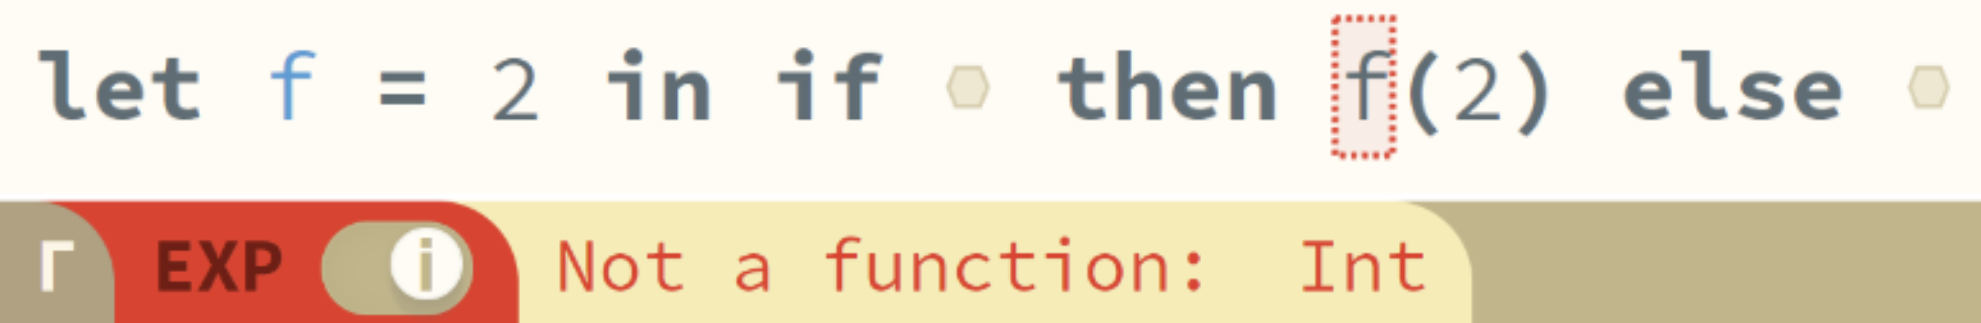
\includegraphics[width=0.9\linewidth]{images/localExCombined.png}
  \label{fig:hazelLocalEx}
\end{subfigure}%
\begin{subfigure}{.5\textwidth}
  \centering
  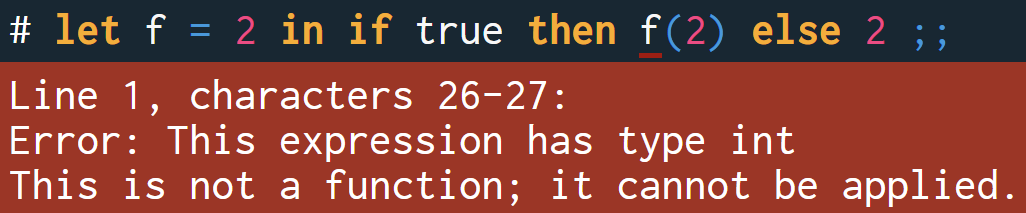
\includegraphics[width=0.9\linewidth]{images/ocamlEx.png}
  \label{fig:ocamlEx}
\end{subfigure}
\caption{Error localization of this program in Hazel and OCaml is similar, but for different reasons.}
\label{fig:localComparison}
\end{figure}

% \begin{figure}[H]
%     \centering
%     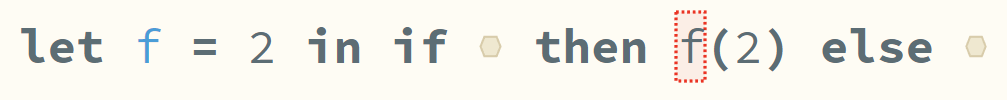
\includegraphics[width=9cm]{images/localEx.png}
%     
\includegraphics[width=9cm]{images/localExCI.png}
%     \caption{A program alongside a localized bidirectional typing error message}
%     \label{fig:enter-label}
% \end{figure}

% We compare the process of user interaction here to that of popular languages like OCaml in \cref{fig:ocaml}. Here, we see that based on the type of the let binding's body, the compiler infers that $f$ has type \verb|int|. Consequently, the error is localized the $f$'s application on 2. In contrast to this, type hole inference allows the user to identify desired annotations while displaying the impact of those choices through subsequent feedback via its bidirectional typing system. This flow is enabled through type hole inference's support of type holes, a mechanism not replicable in OCaml. 

% \begin{figure}[H]
%     \centering
%     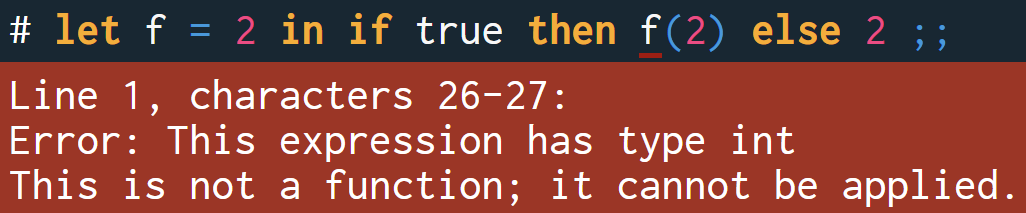
\includegraphics[scale=0.8]{images/ocamlEx.png}
%     \caption{The example program written in OCaml}
%     \label{fig:ocaml}
% \end{figure}

The systems diverge in their capabilities if we explicitly add a type hole annotation to \li{f}. The
bidirectional system treats this as an unknown type and operates gradually, taking this as a signal
that the user has not yet determined the intended type of \li{f}. To help the user fill this type
hole, the system generates and attempts to unify the relevant constraints (see
\cref{sec:unification} below). In this case, the constraints are inconsistent, i.e., there is no hole filling that satisfies all relevant constraints. Rather than favoring constraints arising first, as in OCaml, the type hole itself is highlighted in red and marked with a bang (\li{!}). The user is informed via the Type Inspector that the type hole cannot be solved due to conflicting information from constraints. \Cref{fig:editor_conflict} shows how the editor temporarily fills the type hole when the user hovers over a constraint, deferring to bidirectional error localization as described in Section~\ref{sec:calculus} from there to cause the error to be marked on the \li{2} when hovering over the arrow type.

\begin{figure}[H]
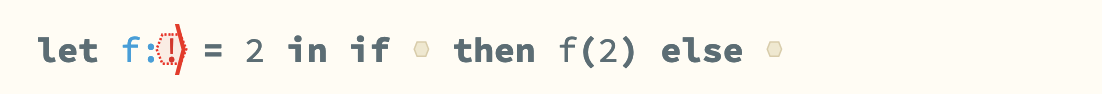
\includegraphics[width=9cm]{images/example_conflict.png}

\includegraphics[width=9cm]{images/example-conflict-newnew.png}
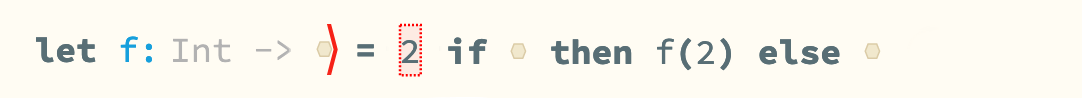
\includegraphics[width=9cm]{images/example_conflict_hover.png}
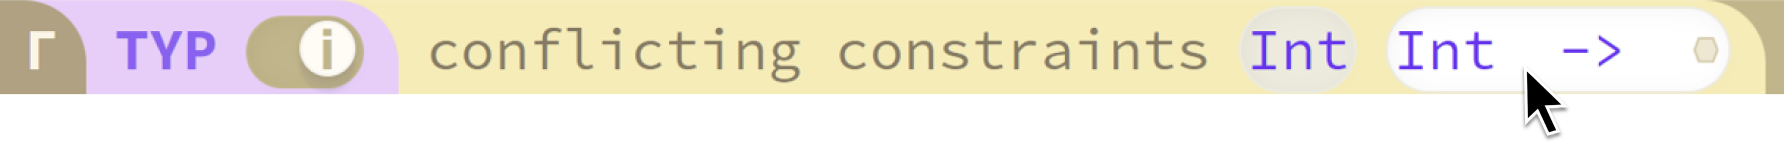
\includegraphics[width=9cm]{images/example-conflict-hover-final.png}
\caption{The error is localized to the conflicted type hole in Hazel. Placing the cursor (\textcolor{red}{$\rangle$}) on the conflicted type hole populates suggestions in the cursor inspector. When hovering over an indicated suggestion, the hole is transiently filled, causing the error to be localized to the bound expression, \li{2}.}
\label{fig:editor_conflict}
\end{figure}
% \begin{figure}[H]
%   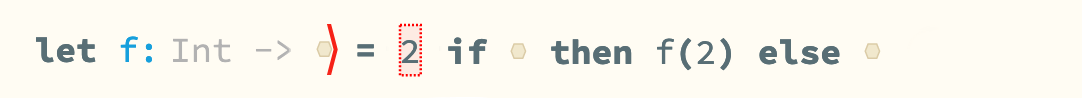
\includegraphics[width=9cm]{images/example_conflict_hover.png}
% 
\includegraphics[width=9cm]{images/example_conflict_hover_CI.png}
% \caption{user hovers over conflicting constraint to show origin [mock-up]}
% \label{fig:editor_conflict_hover}
% \end{figure}

If, given this feedback, the user deletes the bound expression, \li{2}, then there are no longer conflicting constraints on the type hole and the system displays the inferred type in gray, to indicate that it has been inferred rather than entered as ``ground truth'' by the user. The user can press the \li{Enter} key to accept the suggestion (turning the text purple). We depict this flow below in \cref{fig:editor_ghost}. At this point the hole has been filled and localization decisions again become local. Note that there are no constraints on the return type of \li{f}, so the suggested filling itself contains a type hole (see \cref{sec:polymorphicGlobal} below on polymorphic generalization).
\begin{figure}[H]
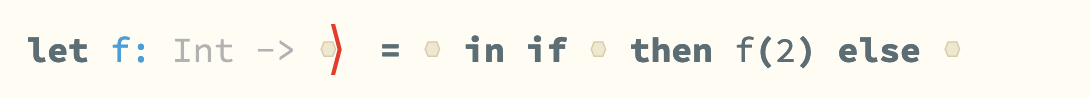
\includegraphics[width=9cm]{images/example_holes_filled.png}

\includegraphics[width=9cm]{images/example_holes_CI.png}
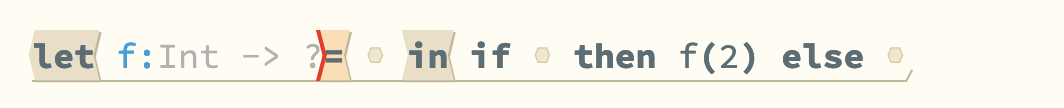
\includegraphics[width=9cm]{images/example_holes.png}
\caption{User removes '2' and accepts the new suggestion}
\label{fig:editor_ghost}
\end{figure}

% \begin{figure}[H]
% 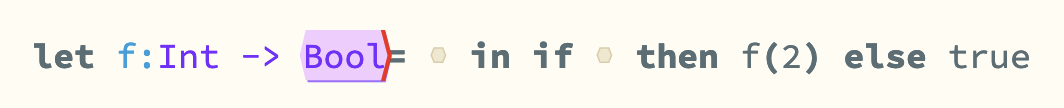
\includegraphics[width=9cm]{images/example_complete.png}
% % 
\includegraphics[width=9cm]{images/example_complete_CI.png}
% \caption{user accepts hole filling suggestion}
% \label{fig:editor_complete}
% \end{figure}

% \subsection{Type Hole Provenance}

% \label{sec:typinf}
% We must be able to uniquely identify type holes when constraint solving because we will treat type holes as type inference variables. Thus, we make two small changes to the marked lambda calculus's syntax:
% \[\begin{array}{rrcl}
%     \Prov & \Provp & \Coloneqq & u \mid exp(u) \mid \rightarrow_L(\Provp) \mid \rightarrow_R(\Provp)\\
%     \TMName  & \TMV  & \Coloneqq & \dots \mid \TUnknown^{p}\\
%     \ECMName & \ECMV & \Coloneqq & \dots \mid \ECFreeId{x}{u} \mid \ECInconTypeId{\ECMV}{u} \mid \ECInconBrId{\ECMV}{\ECMV}{\ECMV}{u} \mid \EEHole^u
% \end{array}\]

% \begin{enumerate}
%     \item We add a unique id $u$ to all expression holes and type holes that appear directly in the program. We assume that id generation is handled by the editor.
%     \item Type holes can also arise internally during constraint generation, below. To identify these, we generalize unique IDs to \emph{provenances}, $p$. These serve two useful but non-critical purposes:
% \begin{enumerate}
%     \item Provenances establish how each type hole connects to some type hole or expression hole
%     that lies in the program. For instance, the provenance $exp(3)$ tells us that this type hole
%     is the synthesized type of the expression hole with id 3 \todo[inline]{this feels somewhat
%     unclear to me; presumably this is the prospective synthesized type of what ends up filling the
%     hole rather than the type of an expression hole (unknown)?}. We discuss the matched arrow
%     provenances below. Future user interface affordances could use provenances to better identify
%     holes, e.g., when internal holes appear in the type or context inspector.\todo[inline]{this is
%     unclear to me. does it mean e.g., jump-to-exp-hole from clicking on a constraint in the CI?}
%     \item Provenances allow increased efficiency when compared to generating fresh type hole ids (which spawns larger constraint graphs during constraint generation.) 
% \end{enumerate}
% \end{enumerate}

It is also worth considering the situation where no type annotation is present, but the bound
expression is an empty expression hole. As an example of this, consider \cref{fig:expLocal}. Here,
the type of \li{x} is unknown according to the bidirectional system from Section~\ref{sec:calculus}.
Type hole inference solves for this unknown type as well, while tracking its provenance as the type
of this expression hole. As such, errors due to conflicting constraints can be localized to
expression holes in much the same way as described above. When the user hovers over a suggested
type, there must be some way of constraining the type of the expression hole, e.g., by finding a suitable variable to annotate with a type or by adding direct ascription syntax to the language (we have not implemented this particular user interface affordance in Hazel as of yet, but there are no fundamental barriers to doing so.) The lightly mocked up process of suggestion is also illustrated below in \cref{fig:expLocal}.

\begin{figure}[H]
    \centering
    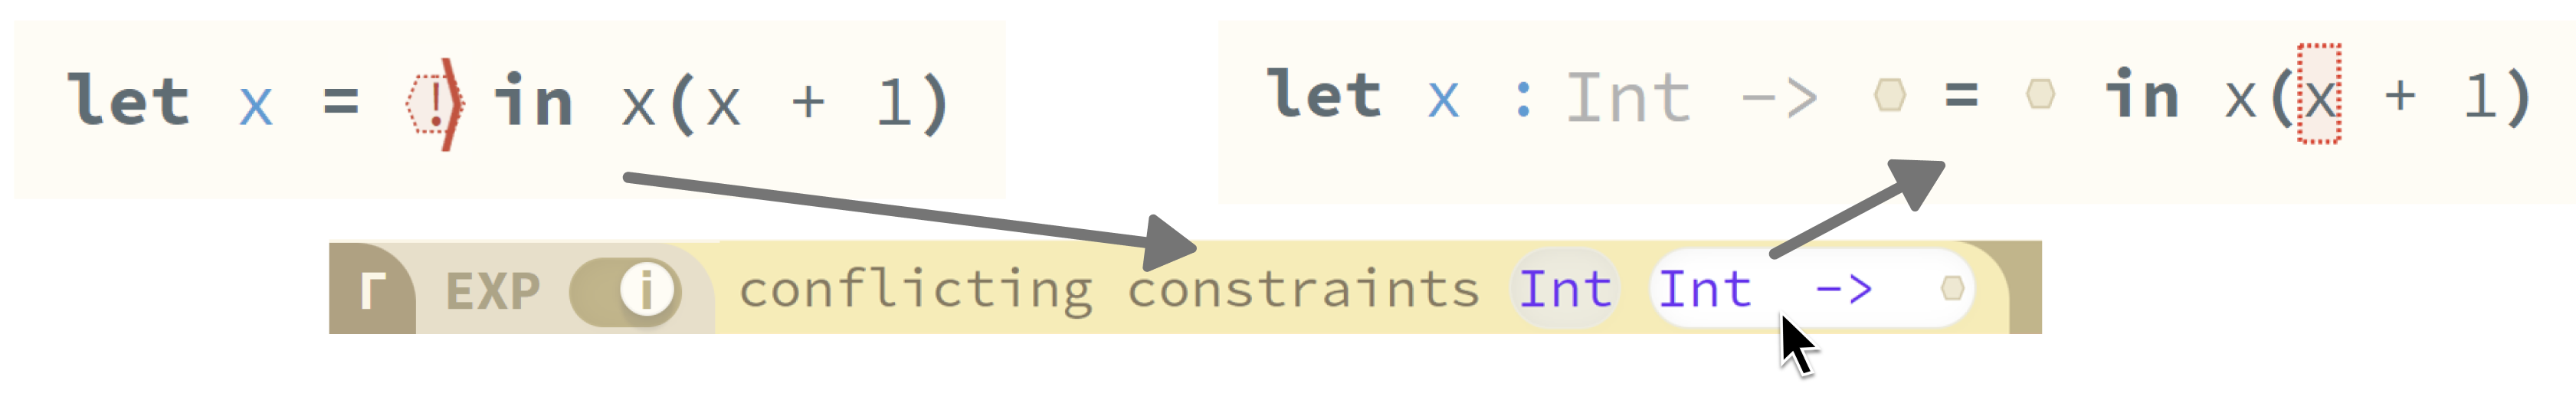
\includegraphics[scale=0.35]{images/expHoleSugg.png}
    \caption{Localization of errors to expression holes.}
    \label{fig:expLocal}
\end{figure}

\subsection{Constraint Generation and Unknown Type Provenance}
In order to generate global inference results, we begin with constraint generation. Our approach
closely follows the usual approach (cf. \cite{pierce2002}), where we augment the bidirectional type system for the marked lambda calculus with generated constraint sets, $C$. The new judgement forms are 
    $\synConstraint{\ctx}{\ECMV}{\TMV}{C}$ and $\anaConstraint{\ctx}{\ECMV}{\TMV}{C}$. 

Constraints, written $\constrain{\tau_1}{\tau_2}$, force two incomplete types to be consistent. Consequently, our rules for constraint generation are quite simple. We augment our previous bidirectional typing rules in the marked lambda calculus to accumulate constraints describing necessary type consistencies. For example, when synthesizing the type of an if expression, we constrain the types of expressions in either branch to each other:
\begin{mathpar}
  \judgment{
    \anaConstraint{\ctx}{\ECMV_1}{\TBool}{C_1} \\
    \synConstraint{\ctx}{\ECMV_2}{\TMV_1}{C_2} \\
    \synConstraint{\ctx}{\ECMV_3}{\TMV_2}{C_3} \\
    \TMV_3 = \TMeet{\TMV_1}{\TMV_2}
  }{
    \synConstraint{\ctx}{\ECIf{\ECMV_1}{\ECMV_2}{\ECMV_3}}{\TMV_3}{C_1 \cup C_2 \cup C_3 \cup \{ \TMV_1 \approx \TMV_2 \}}
  }{MSIf-C}
\end{mathpar}

The remaining rules for standard constructs are similarly standard and given in the supplement.

% For most rules, no new constraints are generated. This leads to straightforward rules like MSLam-C and MSAp1-C:

% \begin{mathpar}
%     \judgment{
%         \synConstraint{\extendCtx{\ctx}{x}{\TMV}}{\ECMV}{\TMV_2}{C}
%     }{
%         \synConstraint{\ctx}{\ECLam{x}{\TMV_1}{\ECMV}}{\TArrow{\TMV_1}{\TMV_2}}{C}
%     }{MSLam-C}

%     \judgment{
%         \synConstraint{\ctx}{\ECMV_1}{\TMV}{C_1} \\
%         \matchedArrowConstraint{\TMV}{\TMV_1}{\TMV_2}{C_2} \\
%         \anaConstraint{\ctx}{\ECMV_2}{\TMV_1}{C_3}
%       }{
%         \synConstraint{\ctx}{\ECAp{\ECMV_1}{\ECMV_2}}{\TMV_2}{C_1 \cup C_2 \cup C_3}
%     }{MSAp1-C}
% \end{mathpar}



Since unification will be solving for unknown types, we must ensure we are able to distinguish between different type holes based on their associated locus in the program. To this end, we make two modifications to the system from Section~\ref{sec:calculus}:

\begin{enumerate}
    \item We add a unique id $u$ to all expression holes and type holes that appear directly in the program where we assume that id generation is handled by the editor.
    \item We add provenances $p$ to unknown types. Each provenance links the unknown type to some (syntactic) hole in the program, perhaps through some intermediate operations. For example, the provenance $exp(3)$ indicates that a type hole must have been synthesized from an expression hole with id $3$ in the program. 
\end{enumerate}
\[\begin{array}{rrcl}
    \Prov & \Provp & \Coloneqq & u \mid exp(u) \mid \rightarrow_L(\Provp) \mid \rightarrow_R(\Provp) \mid \times_L(\Provp) \mid \times_R(\Provp)\\
    \TMName  & \TMV  & \Coloneqq & \dots \mid \TUnknown^{p}\\
    \ECMName & \ECMV & \Coloneqq & \dots \mid \ECFreeId{x}{u} \mid \ECInconTypeId{\ECMV}{u} \mid \dots \mid \ECProjLSynNonMatchedProdId{\ECMV}{u} \mid \ECProjRSynNonMatchedProdId{\ECMV}{u} \mid \EEHole^u
\end{array}\]

Provenance is determined whenever a new unknown type is constructed. For example, we update our matched arrow and product rules to add provenances to outputted type holes and introduce the new matched arrow and product provenances so that every time a matched arrow type is generated for the same hole, it involves the same constituent unknown types without necessitating fresh id generation.
%without needing to introduce explicit constraints:
%edited in response to reviewer C: "I did not understand this, since the rules seem to be adding explicit constraints." 
\begin{mathpar}
    \judgment{ }{
      \matchedArrowConstraint{\TUnknown^p}{\TUnknown^{\rightarrow_L(p)}}{\TUnknown^{\rightarrow_R(p)}}{\{ \TUnknown^p \approx \tarr{\TUnknown^{\rightarrow_L(p)}}{\TUnknown^{\rightarrow_R(p)}} \}}
    }{TMAHole-C}

    \judgment{ }{
      \matchedProdConstraint{\TUnknown^p}{\TUnknown^{\times_{L}(p)}}{\TUnknown^{\times_{R}(p)}}{\{ \TUnknown^p \approx \TProd{\TUnknown^{\times_{L}(p)}}{\TUnknown^{\times_{R}(p)}} \}}
    }{TMPHole-C}
\end{mathpar}

Up until now, we have ignored rules that consider marked errors. This leads us to our second point of interest: what do we do with expressions that have been marked with expression holes? A marked expression has already been deemed erroneous. Therefore, when generating constraints, we do not constrain sub-expressions within a marked hole based on types flowing in from outside the hole. As a simple example of this, we present the standard rule for successful subsumption alongside the rule for subsumption upon the failure of the consistency check:

\begin{mathpar}
    \judgment{
    \synConstraint{\ctx}{\ECMV}{\TMV'}{C} \\
    \consistent{\TMV}{\TMV'} \\
    \subsumable{\ECMV}
  }{
    \anaConstraint{\ctx}{\ECMV}{\TMV}{C \cup \{ \TMV \approx \TMV' \}}
  }{MASubsume-C}
  
    \judgment{
        \synConstraint{\ctx}{\ECMV}{\TMV'}{C} \\
        \inconsistent{\TMV}{\TMV'} \\
        \subsumable{\ECMV}
    }{
        \anaConstraint{\ctx}{\ECInconTypeId{\ECMV}{u}}{\TMV}{C \cup \{ \TMV \approx \TUnknown^{exp(u)} \}}
    }{MAInconsistentTypes-C}
\end{mathpar}

The remaining rules directly follow the intuitions above and are left to the supplemental material.

\subsection{Unification and Potential Type Sets}
\label{sec:unification}

To unify constraints, we use a standard union-find based unification algorithm \cite{huet1976, siek2008}, which accumulates constraint information in \textsf{PotentialTypeSet}s. 

A \textsf{PotentialTypeSet} is a recursive data structure representing \emph{all} of the potential fillings for an associated incomplete type, inferred from type constraints. To facilitate this, rather than  substituting types during unification, which results in a loss of information, we continuously merge \textsf{PotentialTypeSet}s. Since unification treats relations transitively, a property consistency lacks across complete types, we avoid generating \textsf{PotentialTypeSet}s for complete types and simply extend existing \textsf{PotentialTypeSet}s with them as needed.
%
\[\arraycolsep=4pt\begin{array}{rrcl}
\textsf{PotentialTypeSet} & s & \Coloneqq & \textsf{single}(t) \mid \textsf{cons}(t, s) \\
\textsf{PotentialType}    & t & \Coloneqq & \tnum \mid \tbool \mid \tehole^p \mid \tarr{s}{s} \mid \TProd{s}{s}
\end{array}\]
%
These choices allows us to continue past failures and unify any constraints, yielding an accumulated corpus of information on each type hole’s potential solutions and errors through their associated \textsf{PotentialTypeSet}s. Each \textsf{PotentialTypeSet} can be scanned by the editor to identify potential solutions or localize errors as illustrated in \cref{fig:editor_conflict} and \cref{fig:editor_ghost}.

Note again that the novel contribution of this section is not in the particular unification algorithm but rather the architectural decisions that allow us to neatly blend local and constraint-based type inference systems for orthogonal purposes within the same system, and our focus on how to handle inconsistent constraints. As such, we direct the reader to prior work for the algorithmic, formal, and metatheoretic details of unification \cite{siek2008}.

% \subsubsection{Constraints}
% Individual constraints are written $\tau_1 \approx \tau_2$\todo[inline]{might be nice to have a definition box defining this judgement and maybe listing properties}. 
% The relationship that a constraint expresses is not quite consistency, nor is it equality. Rather, if $\tau_1 \approx \tau_2$, $\tau_1$ and $\tau_2$ must have the same solution \todo[inline]{not obvious to me at this point what a 'solution of a type' (vs constraint) refers to} once the constituent type holes are filled. The constraint relation is reflexive and symmetric. It also behaves transitively, but only through type holes and types containing type holes. We refer to such types as "incomplete" types, following \citet{HazelnutPOPL}.

% As an example of the constraint generation process, let us consider the program illustrated in \cref{fig:editor_ghost}. We define an equivalent marked expression $\ECMV_{ex}$ below where the let expression has been replaced with an annotated lambda applied to the let body:
% $$\ECMV_{ex} = \ECAp{(\ECLam{f}{\TUnknown^1}{~~\ECIf{\EEHole^2~}{~(\ECAp{f}{\underline{2}})}{~\EEHole^3}})}{~~\EEHole^0}$$
% What constraints might we expect this expression to generate? In this expression, we expect that the annotation of the lambda is consistent with the type of its argument, $\TUnknown^{exp(0)}$. This notion might generate the constraint $\{ \TUnknown^1 \approx \TUnknown^{exp(0)}\}$. We might further notice that we expect both branches of the if expressions to synthesize consistent types. But what is the type of $\ECAp{f}{\underline{2}}$? Previously, we might have argued that it would simply be $\TUnknown$; however, now we must ask exactly \emph{which} type hole this application synthesizes and determine its provenance. In order to further understand these questions, let us more formally explore constraint generation before revisiting this example.

% \subsubsection{Subsumption Constraints}
% % As discussed earlier, constraints constitute a series of expectations for what different types should be. One key mechanism by which we facilitate our accumulation of these expectations is analysis. Indeed, when we expect something should have a type \TMV, we commonly analyze it against that type. As a classic example of this, consider subsumption. 

% Suppose we have a marked expression \ECMV~ that satisfies the judgement \ctxSynType{\ctx}{\ECMV}{\TMV'} for some context \ctx. If we attempt to analyze \ECMV~ against the type $\tau$, we require, or put another way, we expect, that \consistent{\TMV}{\TMV'}. We extend the rule MASubsume as follows so that it generates the corresponding constraint $\tau \approx \tau'$:
% \begin{mathpar}
%   \judgment{
%     \synConstraint{\ctx}{\ECMV}{\TMV'}{C} \\
%     \consistent{\TMV}{\TMV'} \\
%     \subsumable{\ECMV}
%   }{
%     \anaConstraint{\ctx}{\ECMV}{\TMV}{C \cup \{ \TMV \approx \TMV'\}}
%   }{MASubsume-C}
% \end{mathpar}
% % Notice that we also accumulate constraints generated in each premise in our conclusion.

% One key question is how one should manage constraints whenever marked expressions are marked with
% errors. Should an expected type pass through the mark, which would necessarily create an
% unsolvable constraint? We assert that the answer is no: marks  act as quarantines. We can,
% however, take advantage of the interpretation of marks as non-empty holes to infer a type for the
% marked expression, i.e., the type that mark repair needs to target.

% With this guiding principle in hand, let us approach constraint generation for subsumption when \inconsistent{\TMV}{\TMV'} by extending MAInconsistentTypes:
% \begin{mathpar}
%   \judgment{
%     \synConstraint{\ctx}{\ECMV}{\TMV'}{C}  \\
%     \inconsistent{\TMV}{\TMV'} \\
%     \subsumable{\ECMV}
%   }{
%     \anaConstraint{\ctx}{\ECInconTypeId{\ECMV}{u}}{\TMV}{C \cup \{ \TMV \approx \TUnknown^{exp(u)} \}}
%   }{MAInconsistentTypes-C}
% \end{mathpar}
% % Here, instead of expecting that the type of \ECMV~ be consistent with the type $\tau$, we prevent any conflicts that may arise from $\tau$ reaching beyond our type hole membrane. We then enforce that the hole surrounding \ECMV~ synthesize a type consistent with $\tau$.

% \subsubsection{If Expressions and Their Constraints}
% Expectations for the result of typechecking on expressions is not limited to analysis. Indeed, there are multiple cases where we hold expectations for the types of our expressions in synthesis as well. As a simple example, consider if expressions. We expect that both branches have consistent types and assess this implicitly by attempting to compute their meet. This leads to the following constraint generating rule for if expression synthesis where we simply accumulate constraints and require that $\TMV_1 \approx \TMV_2$:
% \begin{mathpar}
%   \judgment{
%     \anaConstraint{\ctx}{\ECMV_1}{\TBool}{C_1}  \\
%     \synConstraint{\ctx}{\ECMV_2}{\TMV_1}{C_2} \\
%     \synConstraint{\ctx}{\ECMV_3}{\TMV_2}{C_3}
%   }{
%     \synConstraint{\ctx}{\ECIf{\ECMV_1}{\ECMV_2}{\ECMV_3}}{\TMeet{\TMV_1}{\TMV_2}}{C_1 \cup C_2 \cup C_3 \cup \{ \TMV_1 \approx \TMV_2 \}}
%   }{MSIf-C}
% \end{mathpar} 

% Our logic is somewhat trickier when the branches of an if expression have no lower bound, causing it to be wrapped in a marked hole. Inconsistency among branches should be considered an error that lies \emph{within} the hole membrane surrounding our marked expression. Consequently, we constrain $\TMV_1 \approx \TMV_2$ as before and do not consider the type of our hole membrane, $\TUnknown^{exp(u)}$, in the constraints:
% \begin{mathpar}
%   \judgment{
%     \anaConstraint{\ctx}{\ECMV_1}{\TBool}{C_1} \\
%     \synConstraint{\ctx}{\ECMV_2}{\TMV_1}{C_2} \\
%     \synConstraint{\ctx}{\ECMV_3}{\TMV_2}{C_3} \\
%     \inconsistent{\TMV_1}{\TMV_2}
%   }{
%     \synConstraint{\ctx}{\ECInconBrId{\ECMV_1}{\ECMV_2}{\ECMV_3}{u}}{\TUnknown^{exp(u)}}{C_1 \cup C_2 \cup C_3 \cup \{ \TMV_1 \approx \TMV_2 \}}
%   }{MSInconsistentBranches-C}
% \end{mathpar}
% % We assume that the definition of $\TMeet{\TMV_1}{\TMV_2}$ has been adjusted to accept type holes with provenances where we arbitrarily decide that $\TMeet{\TUnknown^{p1}}{\TUnknown^{p2}} = \TUnknown^{p1}$.

% \subsubsection{Matched Arrow Constraints}
% When we generate a matched arrow form for a type hole, we expect that the original type hole be the same as the arrow type outputted by the judgement. Consequently, we find that matched arrow judgements must also accumulate constraints. Thus, we adjust our matched arrow judgement to be of the form $\matchedArrowConstraint{\TMV}{\TMV_1}{\TMV_2}{C}$.

% However, one key question that remains is which provenance to assign the holes outputted by the matched arrow judgement. If we were to simply generate fresh holes ids, they would have no concrete link to the program. To resolve this, we introduce matched arrow provenances, which gives information on why a type hole was created while detailing which type hole it spawned from. 
% Using this, the constraint generating form of TMAHole can constrain the original hole to its matched counterpart while assigning matched arrow provenances to each newly created type hole:
% \begin{mathpar}
% \judgment{ }{
%   \matchedArrowConstraint{\TUnknown^p}{\TUnknown^{\rightarrow_L(p)}}{\TUnknown^{\rightarrow_R(p)}}{\{ \TUnknown^p \approx \tarr{\TUnknown^{\rightarrow_L(p)}}{\TUnknown^{\rightarrow_R(p)}} \}}
% }{TMAHole-C}
% \end{mathpar}

% \subsubsection{Lambda Expressions and Their Constraints}
% Our rule for analysis of annotated lambdas when no local errors are present asserts that the annotation \TMV~ be consistent with the input type of the argument to analysis:
% \begin{mathpar}
%   \judgment{
%     \matchedArrowConstraint{\TMV_3}{\TMV_1}{\TMV_2}{C_1}\\
%     \consistent{\TMV}{\TMV_1} \\
%     \anaConstraint{\extendCtx{\ctx}{x}{\TMV}}{\ECMV}{\TMV_2}{C_2}
%   }{
%     \anaConstraint{\ctx}{\ECLam{x}{\TMV}{\ECMV}}{\TMV_3}{C_1 \cup C_2 \cup \{ \TMV \approx \TMV_1 \}}
%   }{MALam1-C}
% \end{mathpar}

% Our rules for the remaining two lambda analysis cases where the lambda expression is wrapped in a marked hole are trickier. Let us begin by assessing the case where the analyzed type has no matched arrow form. In such cases, we previously analyzed the body of the lambda against the unknown type to ensure its validity. However, which unknown type are we analyzing the body against? As discussed earlier, performing analysis imparts the expectation that the type of the expression is consistent with the argument of analysis. If we were to simply analyze against the type of the hole membrane we use to surround the marked lambda, we'd impart the expectation that the lambda's body is consistent with the hole membrane itself. This would subvert our goal of separating the program outside the hole with that inside!\todo[inline]{i don't totally follow why this reasoning doesnt apply to MALam3-C as well} In fact, any hole we choose would impart some invalid expectation with respect to the goals we've outlined. Consequently, we introduce the anonymous provenance: this will have its constraints ignored by the constraint solver when we later describe unification.
% \begin{center}
%     $\arraycolsep=4pt\begin{array}{lll}
%     \Prov~~ p & ::= & 
%         ... ~\vert~ 
%         anon
%         \\
%     \end{array}$
% \end{center}
% We can analyze the lambda's body against an anonymous unknown type:
% \begin{mathpar}
%   \judgment{
%     \notMatchedArrow{\TMV_3} \\
%     \anaConstraint{\extendCtx{\ctx}{x}{\TMV}}{\ECMV}{\TUnknown^{anon}}{C}
%   }{
%     \anaConstraint{\ctx}{\ECLamAnaNonMatchedArrowId{x}{\TMV}{\ECMV}{u}}{\TMV_3} {C \cup \{ \TUnknown^{exp(u)} \approx \TMV_3 \}}
%   }{MALam2-C}

%   \judgment{
%     \matchedArrowConstraint{\TMV_3}{\TMV_1}{\TMV_2}{C_1}\\
%     \inconsistent{\TMV}{\TMV_1} \\\\
%     \anaConstraint{\extendCtx{\ctx}{x}{\TMV}}{\ECMV}{\TMV_2}{C_2}
%   }{
%     \anaConstraint{\ctx}{\ECInconTypeId{\ECLam{x}{\TMV}{\ECMV}}{u}}{\TMV_3} {C_1 \cup C_2 \cup \{ \TUnknown^{exp(u)} \approx \TMV_3 \}}
%   }{MALam3-C}
% \end{mathpar}
% % Note that the conclusion of these rules add the constraint $\{ \TUnknown^{exp(u)} \approx \TMV_3 \}$. The argument of analysis $\TMV_3$ constitutes an expectation of types from outside the hole surrounding our lambda. Consequently, rather than allowing it to influence the program inside the hole, we simply constrain $\TMV_3$ to the expression hole's type, $?^{exp(u)}$.

% \subsubsection{Applications and Their Constraints}
% This brings us at last to the application of lambdas. When the function position expression $\ECMV_1$ lacks a matched arrow form, we proceed as if we had called\todo{phrasing} matched arrow on the marked expression hole surrounding it. To this end, the function argument $\ECMV_2$ must be analyzed against $\TUnknown^{\rightarrow_L{u}}$ and we must return $\TUnknown^{\rightarrow_R{u}}$ as the result of synthesis. 
% \begin{mathpar}
%   \judgment{
%     \synConstraint{\ctx}{\ECMV_1}{\TMV}{C_1} \\
%     \notMatchedArrow{\TMV} \\
%     \anaConstraint{\ctx}{\ECMV_2}{\TUnknown^{\rightarrow_{L}(exp(u))}}{C_2}
%   }{
%     \synConstraint{\ctx}{\ECApSynNonMatchedArrowId{\ECMV_1}{u}{\ECMV_2}}{\TUnknown^{\rightarrow_{R}(exp(u))}}{C_1 \cup C_2 \cup \{ \TUnknown^{exp(u)} \approx \tarr{\TUnknown^{\rightarrow_L(exp(u))}}{\TUnknown^{\rightarrow_R(exp(u))}}\}}
%   }{MSAp2-C}
% \end{mathpar}

% \subsubsection{Other Constraint Generating Rules}
% The remaining rules either simply accumulate constraints from each of their premises as done above or are axiomatic and need not accumulate any constraints. As a result, they are somewhat repetitive and are consequently left to the supplemental material.\todo[inline]{wordy. instead maybe: 'See supplement for the remaining rules, which either express atomic constraints or simply accumulate the constraints of their premises'}

% \subsubsection{An Example of Constraint Generation}
% Now that we have defined a formal approach to constraint generation, let us revisit $\ECMV_{ex}$ and try once again to identify its constraints:
% $$\ECMV_{ex} \equiv \ECAp{(\ECLam{f}{\TUnknown^1}{~~\ECIf{\EEHole^2~}{~(\ECAp{f}{\underline{2}})}{~\EEHole^3}})}{~~\EEHole^0}$$
% We first consider the body of the lambda, $\ECIf{\EEHole^2~}{~(\ECAp{f}{\underline{2}})}{~\EEHole^3}$. Based on the rule MSIf-C, we must analyze our scrutinee, $\EEHole^2$ against $\tbool$. This triggers subsumption, yielding the constraint $\{ \TUnknown^{exp(2)} \approx \tbool \}$. Next, we must synthesize the types of our branches: $\ECAp{f}{\underline{2}}$ and $\EEHole^3$. Synthesis of $\EEHole^3$ is simple; $\EEHole^3$ synthesizes $\TUnknown^{exp(3)}$ with no constraints.

% Synthesis of $\ECAp{f}{\underline{2}}$ is more complex. Following MSAp1-C, we attempt to take the matched arrow of $\TUnknown^1$, yielding the constraint $\{ \TUnknown^1 \approx \tarr{\TUnknown^{\rightarrow_L(1)}}{\TUnknown^{\rightarrow_R(1)}} \}$. Next, we analyze the argument $\underline{2}$ against the input type of $f$, $\TUnknown^{\rightarrow_L(1)}$. This triggers subsumption, which yields the constraint $\{ \TUnknown^{\rightarrow_L(1)} \approx \tnum \}$. With these results in hand, we can determine that the result of synthesis on  $\ECAp{f}{\underline{2}}$ is $\TUnknown^{\rightarrow_R(1)}$ with constraint set $\{ \TUnknown^1 \approx \tarr{\TUnknown^{\rightarrow_L(1)}}{\TUnknown^{\rightarrow_R(1)}}, ~\TUnknown^{\rightarrow_L(1)} \approx \tnum \}$.

% Combining these results and constraining the types of both branches to each other, we find that $\ECIf{\EEHole^2~}{~(\ECAp{f}{\underline{2}})}{\EEHole^3}$ synthesizes type $\TUnknown^{\rightarrow_R(1)}$ with constraint set $\{ \TUnknown^{exp(2)} \approx \tbool, \TUnknown^1 \approx \tarr{\TUnknown^{\rightarrow_L(1)}}{\TUnknown^{\rightarrow_R(1)}},  \TUnknown^{\rightarrow_L(1)} \approx \tnum,  \TUnknown^{\rightarrow_R(1)} \approx \TUnknown^{exp(3)}\}$. 

% Synthesis of our overarching lambda expression yields no additional constraints and returns the type $\tarr{\TUnknown^1}{\TUnknown^{\rightarrow_L(1)}}$. Application of the lambda on $\EEHole^0$ yields the constraint $\{ \TUnknown^{exp(0)} \approx \TUnknown^{1} \}$ due to subsumption and yields the final type  $\TUnknown^{\rightarrow_R(1)}$. Thus, we find that $\ctxSynType{\cdot}{\ECMV_{ex}}{\TUnknown^{\rightarrow_R(1)}} ~|~ C_{ex1}$ where 
% $$C_{ex1} = \{ \TUnknown^{exp(2)} \approx \tbool, \TUnknown^1 \approx \tarr{\TUnknown^{\rightarrow_L(1)}}{\TUnknown^{\rightarrow_R(1)}},  \TUnknown^{\rightarrow_L(1)} \approx \tnum, \TUnknown^{exp(0)} \approx \TUnknown^{1}, \TUnknown^{\rightarrow_R(1)} \approx \TUnknown^{exp(3)} \}$$

% \todo[inline]{i wonder if this section can be made more incremental. like, if the rules were introduced in the order in which they are required for the derivation of the motivating example, then you could interleave the rules with this derivation sketch. as it stands, i feel like i've forgotten the motivating example by the time i get here, whereas the other way it could serve to generate explicit sub-examples for the relevant rules. right now i feel this part at the end is a bit of an awkward balance of symbolic and conversational}

%%%%%%%%%%%%%%%%%%%%%%%%%%%%%%%%%% INFERENCE ALGORITHM %%%%%%%%%%%%%%%%%%%%%%%%%%%%%%%%

% \usetikzlibrary{positioning,calc}

% \subsection{Constraint Solving with Recovery}
% \label{sec:infalg}
% The problem of inferring types from constraints has been widely explored in the literature. In the spirit of Hazel, which allows users to program with holes and even run incomplete programs, it would be beneficial to provide holistic type-related feedback for all edit states. With this in mind, we approach type inference with the key goal of representing all potential type fillings for type holes, regardless of any conflicts that may arise during unification.

% In order to do this, we begin with a simpler problem: representing our constraints as an undirected graph. We'd like to construct our constraint graph such that if a node for some type hole $\TUnknown^{p_1}$ can be reached from the node for $\TUnknown^{p_2}$, it must be the case that $\TUnknown^{p_1} \approx \TUnknown^{p_2}$. Once we have a graph of all constraints, the problem of identifying potential types to suggest for any type hole in the program can be boiled down to that of identifying our graph's connected components. Put another way, if we want to find the potential types that may be used to fill some type hole, all we need to do is find all nodes that can be reached from it in the constraint graph.

% It is important to note that before we begin constructing constraint graphs, we must filter all constraints involving the anonymous type hole $?^{anon}$. While necessary for certain edge cases in type checking, the anonymous type hole represents an inherent lack of expectations. Consequently, all constraints involving it can be ignored.

% \subsubsection{Approaches to Constructing Constraint Graphs}
% When constructing a graph of our constraints, our first inclination  might be to allow all types found in our constraints to act as nodes in our graph. We could then create a traversable edge between nodes for every constraint. However, such a choice prevents pairs that are reachable from one another from always being related via the constraint relation. To see why, recall that the constraint relation is only transitive across incomplete types (those containing at least one type hole). Since edges can be traversed transitively, we cannot have traversable edges between all types represented in constraints. Rather, only incomplete types can be linked by traversable edges. Conversely, complete types should only be reachable through incomplete types that have been directly constrained to them. 

% To simplify this observation, we assert that only incomplete types can be nodes in our graph. We refer to edges connecting incomplete types as \emph{traversable edges} and draw them as solid lines. Edges linking to complete types will be represented via \emph{solution edges}, which we draw as dashed lines. These edges can only be used to discover complete types and can never be used to travel through them. As a result, complete types cannot be used as a layover between incomplete types. 

% As an example of this, consider \cref{fig:ex2ex3graphs}. \Cref{fig:reachable-tag} illustrates a set of constraints $C_{ex2} = \{ \tehole^{1} \approx \tnum, ~ \tehole^{1} \approx~ \tehole^{2}\}$ where all nodes can be solved as $\tnum$ by discovering $\tnum$ through $\tehole^1$. Consequently, this graph has a single connected component. On the other hand, \cref{fig:disjoint-nodes} illustrates an example set of constraints $C_{ex3} = \{ \tehole^1 \approx \tnum, ~ \tehole^1 \approx \tbool, ~ \tnum \approx~ \tehole^2\}$ where $\tnum$ is discovered by two separate incomplete types, but cannot be used to connect them. Consequently, it contains two connected components. 

% \begin{figure}[htb!]
% \centering
% \begin{subfigure}{.49\textwidth}
%   \centering
%       \begin{tikzpicture}
%       [scale=.8,auto=left,every node/.style={circle,fill=blue!20}]
%       \node[rectangle,minimum size=0.85cm] (n1) at (3,3) {$\tehole^{1}$};
%       \node[rectangle,minimum size=0.85cm] (n2) at (1,3)  {$\tehole^{2}$};
%       \node[minimum size=0.85cm] (i) at (3,1)  {$\tnum$};
    
%       \foreach \from/\to in {n1/n2}
%         \draw (\from) -- (\to);
%        \foreach \from/\to in {n1/i}
%         \draw[dashed] (\from) -- (\to);
    
%     \end{tikzpicture}
%   \caption{Graph of $C_{ex2} = \{ \tehole^{1} \approx \tnum, ~ \tehole^{1} \approx~ \tehole^{2}\}$}
%   \label{fig:reachable-tag}
% \end{subfigure}
% \begin{subfigure}{.49\textwidth}
%   \centering
%   \begin{tikzpicture}
%   [scale=.8,auto=left,every node/.style={circle,fill=blue!20}]
%   \node[rectangle,minimum size=0.85cm] (n1) at (2,3) {$\tehole^{1}$};
%   \node[rectangle,minimum size=0.85cm] (n2) at (4,3)  {$\tehole^{2}$};
%   \node[minimum size=0.85cm] (i1) at (4,1)  {$\tnum$};
%   \node[minimum size=0.85cm] (i2) at (2,1)  {$\tnum$};
%   \node[minimum size=0.85cm] (i3) at (0,3)  {$\tbool$};

%    \foreach \from/\to in {n1/i3, n1/i2, n2/i1}
%     \draw[dashed] (\from) -- (\to);

% \end{tikzpicture}
%   \caption{Graph of $C_{ex3} = \{ \tehole^1 \approx \tnum, ~ \tehole^1 \approx \tbool, ~ \tnum \approx~ \tehole^2\}$}
%   \label{fig:disjoint-nodes}
% \end{subfigure}
% \caption{Sample constraint graphs of ground types}
% \label{fig:ex2ex3graphs}
% \end{figure}

% % Constructing a graph of type nodes and adding edges between them has an important caveat: Only $\tehole^{p}$ or types containing at least one $\tehole^{p}$ are added to the graph as nodes. See Figure \ref{fig:ex1ex2graphs} for an illustration. In part (a) of Figure \ref{fig:ex1ex2graphs}, $\tehole^{1}$ and $\tehole^{2}$ are nodes in the graph \textit{linked} by a solid edge, and $\tnum$ is not. Instead, $\tnum$ is more like a \textit{tag} adding additional type information to $\tehole^{1}$. Hence, we use a dotted edge in the illustration to represent this distinction. Since $\tnum$ is constrained to $\tehole^{1}$, the solver can infer using union-find that $\tehole^{2}$ must also contain $\tnum$ in its \textit{PotentialTypeSet}, because $\tehole^{1}$ and $\tehole^{2}$ are part of the same connected component. By contrast, in part (b), $\tehole^{1}$ and $\tehole^{2}$ are both \textit{tagged} with $\tnum$, but because they are not part of the same connected component, the solver will not infer that they share the same \textit{PotentialTypeSet}. Consequently, the solver will correctly not infer that $\tehole^2$ contains $\tbool$ in its \textit{PotentialTypeSet}.

% Upon encountering a constraint between two arrow types, we can generate two new constraints on-the-fly: one between the left children of the arrows, and one between the right children of the arrows. For example, given the constraint set $C_{ex4} = \{ \tarr{\tehole^1}{\tehole^2} \approx \tarr{\tehole^3}{\tnum} \}$, we generate the constraints $\tehole^1 \approx \tehole^3$ and $\tehole^2 \approx \tnum$. These constraints can then be used to render the graph depicted in \cref{fig:arrowgraph}. Here, we represent incomplete $Arrow$s as nodes whose types are dependent on their left and right hand sides, which may also be nodes. As an example, we see in \cref{fig:arrowgraph} that $\tarr{\tehole^1}{\tehole^2}$ is represented by a large arrow node containing the node $\tehole^1$ on the left and $\tehole^2$ on the right. 
% % Any node linked to an $Arrow$ node can only access its left and right hand sides once they are paired together and wrapped in a binary $\rightarrow$ type. 

% With these rules in hand, we can construct graphs for more complex constraint sets. Let us explore the graph of the constraint set $C_{ex1}$ generated from the synthesis of $\ECMV_{ex}$ in section 4.4.8:
% $$C_{ex1} = \{ \TUnknown^{exp(2)} \approx \tbool, \TUnknown^1 \approx \tarr{\TUnknown^{\rightarrow_L(1)}}{\TUnknown^{\rightarrow_R(1)}},  \TUnknown^{\rightarrow_L(1)} \approx \tnum, \TUnknown^{exp(0)} \approx \TUnknown^{1}, \TUnknown^{\rightarrow_R(1)} \approx \TUnknown^{exp(3)} \}$$
% We provide an illustration of this constraint graph in \cref{fig:C-ex-graph-traversal}. The red edges in \cref{fig:C-ex-graph-traversal} represent all paths that may be followed beginning at $?^1$. 

% Suppose we wanted to generate a suggestion for $?^1$ using this graph. This could be achieved by simply traversing all red edges in \cref{fig:C-ex-graph-traversal} to discover potential types. Note that potential types discovered within the left and right hand side of the $Arrow$ node must be wrapped pairwise in an $\rightarrow$ type before being added to $?^1$'s list of potential types. Following these edges generates the following set of potential types for $?^1$: $\{  ?^0, ?^1, \tarr{\tnum}{?^3}, \tarr{\tehole^{\rightarrow_{L(1)}}}{?^3}, \tarr{\tnum}{\tehole^{\rightarrow_{R(1)}}}, \tarr{\tehole^{\rightarrow_{L(1)}}}{\tehole^{\rightarrow_{R(1)}}}  \}$. Notice that after exploring the arrow, our number of potential types have grown rapidly!

% \begin{figure}[htb!]
% \centering
% \captionsetup[subfigure]{justification=centering}
% \begin{subfigure}{.49\textwidth}
%         \centering
%       \begin{tikzpicture}[remember picture,
%   inner/.style={rectangle,draw=blue!50,fill=blue!20,thick,inner sep=3pt,minimum size=0.85cm},
%   innercirc/.style={circle,draw=blue!50,fill=blue!20,thick,inner sep=3pt,minimum size=0.85cm},
%   outer/.style={draw=green,fill=green!20,thick,inner sep=10pt}
%   ]
%   \node[outer,draw=green] (A) {
%     \shortstack{
%         $Arrow$\\
%         \begin{tikzpicture}
%           \node [inner] (n1)  {$\tehole^{1}$};
%           \node [inner,right=of n1] (n2) {$\tehole^{2}$};
%           % \draw[red,thick,->] (n1) -- (n2);
%         \end{tikzpicture}
%     }
%   };
%   \node[outer,draw=green,below=of A] (B) {
%     \shortstack{
%         $Arrow$\\
%         \begin{tikzpicture}
%           \node [inner] (n3)  {$\tehole^{3}$};
%           \node [innercirc,right=of n3] (i) {$\tnum$};
%           % \draw[red,thick,->] (n3) -- (i);
%         \end{tikzpicture}
%     }
%   };
%   \draw (n1) -- (n3);
%   \draw[dashed] (n2) -- (i);
%    \draw[thick] (A) -- (B);
% \end{tikzpicture}
% \caption{Expanded constraint graph of\\ $C_{ex3} = \{ \tarr{\tehole^1}{\tehole^2} \approx \tarr{\tehole^3}{\tnum} \}$}
% \label{fig:arrowgraph}
% \end{subfigure}
% \begin{subfigure}{.49\textwidth}
%   \centering
%   \begin{tikzpicture}[remember picture,
%   tag/.style={circle,draw=blue!50,fill=blue!20,thick,inner sep=3pt,minimum size=0.85cm},
%   holey/.style={rectangle,draw=blue!50,fill=blue!20,thick,inner sep=5pt,minimum size=0.85cm},
%   outer/.style={draw=green,fill=green!20,thick,inner sep=10pt},
%   ]
%   \node[holey] (hole1) {$\tehole^1$};
%   \node[holey, right=of hole1] (hole0) {$\tehole^0$};
%   \node[outer, below=of hole1] (Arrow) {
%     \shortstack{
%         $Arrow$\\
%         \begin{tikzpicture}
%           \node [holey] (holeL1)  {$\tehole^{\rightarrow_{L(1)}}$};
%           \node [holey, right=of holeL1] (holeR1) {$\tehole^{\rightarrow_{R(1)}}$};
%         \end{tikzpicture}
%     }
%   };
%  \node[tag, below=of holeL1] (num) {$\tnum$};
%  \node[holey, below=of holeR1] (hole3) {$\tehole^3$};
%  \node[holey, right=of holeR1] (hole2) {$\tehole^2$};
%  \node[tag, below=of hole2] (bool) {$\tbool$};
%   \draw[draw=red] (hole1) -- (hole0);
%   \draw[draw=red] (hole1) -- (Arrow);
%   \draw[dashed, draw=red] (num) -- (holeL1);
%   \draw[draw=red] (hole3) -- (holeR1);
%   \draw[dashed] (bool) -- (hole2);
% \end{tikzpicture}
% % \caption{Constraint graph of\\ 
% % $C_{ex1} = \{ \TUnknown^{exp(2)} \approx \tbool, \TUnknown^{exp(0)} \approx \TUnknown^{1},$ \\
% % $\TUnknown^1 \approx \tarr{\TUnknown^{\rightarrow_L(1)}}{\TUnknown^{\rightarrow_R(1)}},  \TUnknown^{\rightarrow_L(1)} \approx \tnum,$ \\
% % $\TUnknown^{\rightarrow_R(1)} \approx \TUnknown^{exp(3)} \}$}
% \caption{Constraint graph of $C_{ex1}$}
% \label{fig:C-ex-graph-traversal}
% \end{subfigure}
% \caption{Sample constraint graphs including binary types}
% \label{fig:ex1ex2graphs}
% \end{figure}

% \subsubsection{PotentialTypeSets and the Graph Construction Algorithm}
% Now that we have a clear approach to generating constraint graphs, how might we represent the types that are adjacent to each node? One approach would be to simply store an adjacency list or matrix. However, we'd like to be able to efficiently store all potential hole fillings that can be derived from a type hole's connected components. Recall the rapid growth of potential types discovered for $?^1$ from the graph of $C_{ex1}$ in \cref{fig:C-ex-graph-traversal}. Since the set of potential types can grow at a combinatorial rate, we define a new, condensed data structure to house our potential type hole fillings without loss of information: a \emph{PotentialTypeSet}.

% A \textit{PotentialTypeSet} is a recursive data structure representing the potential solutions for a type hole, inferred from type constraints. A single \emph{PotentialTypeSet} contains \emph{all} of the potential fillings for its associated type hole. To facilitate this, rather than ever substituting types during unification, which results in a loss of information, we continuously extend some \emph{PotentialTypeSet}. We provide a formalization of \textit{PotentialTypeSet}, \textit{PotentialType}, and their extension below in \cref{fig:possible_type_sets}.

% \begin{figure}[hbt!]
% \centering
% \vspace{-3px} 
% $\arraycolsep=4pt\begin{array}{lll}
% PotentialTypeSet~~ s & ::= 
% single(t) ~\vert~ 
% cons(t, s)
% \\
% PotentialType~~ t & ::= 
%   \tnum ~\vert~
%   \tbool ~\vert~
%   \tehole^p ~\vert~
%   \tarr{s}{s}
%   \\
% \end{array}$
% \label{fig:syntax_possible_type_sets}
% \vspace{5px}
% \hrule
% \[\begin{array}{rcl}
%     single(\tarr{s_1}{s_2}) ~\amalg~ single(\tarr{s_3}{s_4}) & = & single({\tarr{(s1 ~\amalg~ s3)}{(s2 ~\amalg~ s4)}}) \\
%     single(t) ~\amalg~ single(t') & = & cons(t, single(t')) \\
%     cons(t,s) ~\amalg~ single(t) & = & cons(t, s) \\
%     cons(\tarr{s_1}{s_2}, s) ~\amalg~ single(\tarr{s_3}{s_4}) & = & cons(\tarr{(s1 ~\amalg~ s3)}{(s2 ~\amalg~ s4)} , s) \\
%     cons(t,s) ~\amalg~ cons(t',s') & = & cons(t,s) ~\amalg~ single(t') ~\amalg~ s' \\
% \end{array}\] 
% \caption{Syntax of PotentialTypeSets, PotentialTypes, and their Merging}
% \vspace{5px} 
% \label{fig:possible_type_sets}
% \vspace{-5px}
% \end{figure}

% With this in hand, we formalize the intuitions discussed in section 4.5.1 in a graph construction algorithm. This algorithm accumulates a mapping from incomplete types, which represent our nodes, to their \emph{PotentialTypeSet}, which represents a subset of nodes reachable from a given incomplete type. Whenever we attempt to create a traversable edge or a solution edge between nodes, we retrieve the \emph{PotentialTypeSet}s of all involved nodes, compute the result of merging them, and update our graph accordingly. We assume the existence of a \lstinline{Map.add} function that adds a new element to the supplied map if it does not already exist, and otherwise does not change any values. The corresponding definition is provided in \cref{fig:algcode_construct_graph}

% \begin{figure}[hbt!]
% \begin{lstlisting}[escapeinside={(*}{*)}]
% let rec construct_graph (~graph=Map.empty(), constraints) =
%     match constraints with
%     | [] -> graph
%     | hd::tl -> (
%         (match hd with
%         | ((*$\tarr{t1_L}{t1_R}$*), (*$\tarr{t2_L}{t2_R}$*)) ->
%             construct_graph(~graph, (((*$t1_L$*), (*$t2_L$*)))::(((*$t1_R$*), (*$t2_R$*)))::tl)
%         | ((*$\tehole^{p}$*) as hole, t)
%         | (t, (*$\tehole^{p}$*) as hole) ->
%             let graph = Map.add(graph, hole, hole) in
%             if (contains_hole(t)) then (
%                 let graph = Map.add(graph, t, t) in
%                 let graph = create_traversable_edge(graph, t, hole) in
%                 construct_graph(~graph, tl)
%             ) else (
%                 let graph = create_solution_edge(graph, hole, t) in
%                 construct_graph(~graph, tl)
%             )
%         | _ -> construct_graph(~graph, tl))

% \end{lstlisting}
% \hrule
% \caption{Constraint graph creation algorithm of type hole inference}
% \label{fig:algcode_construct_graph}
% \end{figure}

% \subsubsection{Computing PotentialTypeSets Using Constraint Graphs} 
% The function \lstinline{construct_graph} builds a mapping from each type hole to a \emph{PotentialTypeSet} containing a subset of its connected component. However, in order to generate all potential type hole fillings, we require that each \emph{PotentialTypeSet} represent the entire connected component. One method to expand our \emph{PotentialTypeSet}s would be to conduct a depth first search of our graph. Instead of this, we choose to simply augment our current approach using union find, yielding a version of \lstinline{construct_graph} that is reminiscent of Huet's unification algorithm \cite{Huet}.

% In order to change our graph construction algorithm to a constraint solver, all we need to do is update our definitions of \lstinline{create_traversable_edge} and \lstinline{create_solution_edge} to use represent each potential type set using union find. In order to accommodate this change, minor adjustments must be made to the definitions presented in \cref{fig:possible_type_sets} to create union findable possible type sets and their extension logic, $\amalg_{UF}$. These definitions are left to the supplemental material for reference.

% An additional step is taken to mark type holes with an error if their \emph{PotentialTypeSet} contains a cycle that is not a self loop. In Hindley-Milner type inference this is referred to as the occurs-check.

% After our union find based \lstinline{construct_graph} and occurs check marking have been completed, we are ready to identify the solvability of our type holes. We consider type holes solvable if their \textit{PotentialTypeSet} contains at most one type that is not a hole. On the other hand, if a type hole's \textit{PotentialTypeSet} contains multiple conflicting types, or if the type hole fails the occurs check, then it is considered unsolvable. In both cases,  feedback can be provided as in \cref{fig:editor_conflict}.

% % \subsubsection{Other Binary Types}
% % Suppose we wanted to extend our definitions of constraint generation and solving to contain binary products as discussed in section 2.2. This would require an extension of our constraint generation rules and definitions of \emph{PotentialTypeSet}s. We follow the same procedures in section 4.4 and introduce a new matched product judgement that constrains inputted holes to their matched product form. In order to extend \emph{PotentialTypeSet}s to support binary products, we must slightly adjust our definitions to be more general across different binary type operators. The resulting rules are very similar to those discussed earlier, and are also consequently left for review in the supplemental material.

\subsection{Polymorphic Generalization with Holes}
\label{sec:polymorphicGlobal}
% In order to extend our definitions of \emph{PotentialTypeSet}s to allow parametric polymorphism, we simply include a new ground type: $\TVar$.
% \begin{center}
% $\arraycolsep=4pt\begin{array}{lll}
% PotentialType~~ t & ::= 
%   \dots \mid \TVar
% \end{array}$
% \end{center}
% By representing all type variables this way, we enforce that type variables are only consistent with type holes and each other. 
In many type inference systems, unconstrained type inference variables (here, unknown types) are automatically polymorphically generalized, so that
functions can be given the most general type \cite{garcia2015}. The same approach can be taken with type hole inference, but with one particularly interesting wrinkle. With the inclusion of expression holes in our system, we need to be a bit more careful about when we generalize. Consider the following expression:
$$\ECLam{x}{\TUnknown^1}{\EEHole^2}$$
We can see that $\TUnknown^1$ is not constrained. Suppose that we were to suggest the implicitly universally quantified type variable $'a$ as a type hole filling for $?^1$. It is unlikely that the user accepts this suggestion because it is unlikely that the user intends to write the identity function!
The fact there are not yet any constraints does not imply that there will not be once the expression hole is filled.

To address this, we need to reason as if there are any number of \emph{unknown constraints} coming from expression holes.  This can be represented with a new type of constraint: the $\mathtt{etc}$ constraint, which we add to our syntax of \textsf{PotentialType}s below. 
\begin{center}
$\arraycolsep=4pt\begin{array}{rrcl}
  \textsf{PotentialType} & t & \Coloneqq & \dots \mid \mathtt{etc}
\end{array}$
\end{center}
When an expression hole appears, all unknown types in the typing context are constrained to $\mathtt{etc}$. This has no impact on unification, but if a type hole $?^p$ is constrained to $\mathtt{etc}$, it cannot be generalized. As before, more expansive discussion on unification with gradual typing including polymorphism is left to prior work \cite{garcia2015}.

% \subsubsection{User Interaction and Conflict Highlighting}
% To further the goal of helping users repair their programs, it would be beneficial to assign blame by highlighting the portions of the program responsible for the unsolved status of a \textit{PotentialTypeSet}. To allow this, constraints could be extended to contain the unique identifier of the expression from which they originated. Highlighting all expressions of the program which resulted in an unsolved \textit{PotentialTypeSet}, rather than attempting to localize the error to one particular expression, would result in less confusion and give the user more clues to discover the true source of a type error.
%These identifiers effectively act as reasons for edges within our constraint graph, enabling us to describe the exact series of reasons that caused the inference algorithm to conclude a type hole's solution status.




\section{Related Work}
\label{sec:related}

The contributions of this paper build directly on the Hazelnut type system \cite{omar2017b}, which is discussed extensively throughout. Non-empty holes in Hazelnut generalize to marks in this work. In brief, we contribute a total marking procedure (Section~\ref{sec:calculus}) and type hole inference scheme (Section~\ref{sec:thi}) for a system based closely on Hazelnut, and use it to fix some expressiveness issues in Hazelnut's edit action calculus (Section~\ref{sec:calculus-structured-editing}). 

Hazelnut is in-turn rooted in gradual type theory \cite{siek2006, siek2015}. We make extensive use of (only) the static aspects of gradual typing---namely, the universal consistency of the unknown type---to enable recovery from marked errors, which can leave missing type information.

Our focus was exclusively on static typing in this paper, and the results are relevant to the design of language servers for any statically typed language, but it is worth noting that the results in this paper, taken together with Hazel's support for maintaining syntactic well-formedness using structure editing \cite{moon2023,moon2022} and for running programs with holes and marked errors \cite{omar2019}, allow our implementation of Hazel to achieve \emph{total liveness}: every editor state is syntactically, statically, and dynamically meaningful, without gaps.

Type error localization is a well-studied problem in practice. This paper is the first to formally support the intuition that, in the words of \citet{dunfield2019}, ``bidirectional typing improves error locality.'' Although there has been considerable folklore around error localization 
for systems with local type inference, the problem has received little formal attention. We hope that this paper, with its rigorous formulation
of type error localization and recovery for bidirectionally typed languages, will provide more rigorous grounding to language server development,
much as bidirectional typing has done for type checker development.

For systems rooted in constraint solving, there has been considerable work in improving error localization because such systems are notorious for making error localization difficult, and programmers are often confused by localization decisions \cite{wand1986} because they are rooted in \emph{ad hoc} traversal orders \cite{mcadam1999,lee1998}. 
More recently, there has been a series of papers that discuss finding the most likely location for an error based on a maximum likelihood criterion applied to type flows \cite{zhang2014} or manual/learned weights \cite{pavlinovic2014,seidel2017}.
While improving the situation somewhat, these remain fundamentally \emph{ad hoc} in their need to guess the user's likely intent. However, these approaches could perhaps be layered atop type hole inference to improve the ranking or filtering of suggestions.

A more neutral alternative is to derive a set of terms that contribute to an error, an approach known as type error slicing \cite{haack2003,tip2001,schilling2011}. This creates a large amount of information for the programmer to consume. Our approach is to instead simply report the constraint inconsistencies on a hole in the program and allow for the programmer to interactively refine their intent, so only the bidirectional type system is responsible for identifying particular erroneous expressions. We do not make particular usability claims about the interactive affordances related to type hole inference in this paper, but rather simply claim a novel neutral point in the overall design space that uniquely combines local and global approaches.

Recent work on gradual liquid type inference described an exploratory interface for filling holes in refinement types by selecting from partial solutions to conflicting refinement type constraints \cite{vazou2018}. This is similar in spirit to type hole inference as described in this paper, albeit targeting program verification predicates.

The underlying unification algorithm is essentially standard---the novelty is in how the unification results are used and how failures are handled, rather than in the inference itself. In particular, we base our approach on the system described by \citet{siek2008}, because it also identifies type inference variables with the unknown type from gradual typing and the union find data structure is useful for computing possible type sets. \citet{garcia2015} similarly present a static implicitly typed language, where users opt into dynamism by annotating an expression with the gradual type "?", and an associated type inference algorithm and accompanying metatheory. By contrast, the Hazelnut type system assigns gradual types to programs that would ordinarily not type-check in a non-gradual system by wrapping them in expression holes. The type inference algorithm presented in \citet{garcia2015} also does not specify what to do if the constraint set cannot be solved. If a single static type cannot be determined for an expression, its type is simply undefined, whereas our approach provides a list of suggestions derived from any conflicting constraints if a single substitution cannot be determined. As our focus is on failure cases and partially consistent suggestions, the metatheory in this prior work is less relevant in guiding the design of the type hole inference system.

Of note, however, is that approaches that eagerly solve and substitute for type inference variables \cite{odersky1999,pottier2014,mcadam1999} are not well-suited to the type hole inference approach, as they lose information necessary for computing partially consistent suggestions. 

% In addition to type error localization and recovery, type hole inference touches on the problem of type error repair, as has been considered by other work \cite{lerner07}. We hope that our work will drive future work on rigorous repairs.

In the realm of error messages for constraint-based inference, work on the Helium Haskell compiler \cite{heeren2003} offers two constraint solvers based on the desired feedback: a global, type graph-based constraint solver which provides detailed error messages, and a lightweight and high-performance greedy solver. When using the global constraint solver, various heuristics can tune the likelihood of different parts of programs reported as error sources.
Recently, \citet{bhanuka2023} model the flow of type information throughout the program using subtyping constraints to produce detailed error messages when unification fails. \citet{seidel2016} provide sample inputs (dynamic witnesses) that elicit runtime errors. With this approach, one can generate graphs for visualizing the execution of witnesses and heuristically identify the source of errors with around 70\% accuracy.
Our focus in this paper has not been on the error messages displayed on-screen, about which we make no specific claims.
It may, however, be beneficial in future work to indicate to the user from where in the program type suggestions originated via our type provenances and by incorporating the techniques in this prior work, e.g. to explain why a particular suggestion arises. 
% Note that documenting the flow of type information would require using asymmetric constraints rather than typical bidirectional equality constraints. 

\section{Conclusion}
\label{sec:conclusion}

\begin{quote}
    \emph{Nothing will ever be attempted if all possible objections must first be overcome.} 
    \begin{flushright}-- Samuel Johnson\end{flushright}
\end{quote}

Programming is increasingly a live collaboration between human programmers and sophisticated semantic services. These services need to be able to reason throughout the programming process, not just when the program is formally complete. This paper lays down rigorous type-theoretic foundations for doing just that. Bidirectional type checking helps make the localization decisions we make systematic and predictable, and type hole inference shows how local and constraint-based type inference might operate hand-in-hand, rather than as alternatives. Throughout, we focused on maintaining neutrality about user intent whenever possible. 
We hope that language designers will use the techniques introduced in this paper to consider more rigorously, perhaps even formally, the problems of type error localization and error recovery when designing future languages. 

\section*{Data Availability Statement}
An artifact \cite{zhao2023} containing the complete formalization of the marked lambda calculus and the extensions described above, the Agda mechanization, and the implementation of Hazel including type hole inference is available.
Up-to-date versions of the formalism and mechanization may be found at \url{https://github.com/hazelgrove/error-localization-agda}.
Hazel is being actively developed---more information is available at \url{https://hazel.org}, and the Hazel source code is maintained at \url{https://github.com/hazelgrove/hazel}.

\section*{Acknowledgements}
The authors would like to thank the anonymous referees at POPL 2024 and ICFP 2023 for helpful feedback on earlier drafts of this paper.
This work was partially funded through the NSF grant \#CCF-2238744.

% Thank you for reading this paper!


\bibliography{typeholeinference_references}

\end{document}
